\documentclass[a4paper,12pt]{report}
\usepackage[utf8]{inputenc}
\usepackage{fontenc}
\usepackage[french, arabic]{babel} % If you write in French
\usepackage{a4wide}
\usepackage{graphicx}
\usepackage{placeins}
%pour la mise en page des tableaux
\usepackage{array}
\usepackage{tabularx}
\usepackage[table,xcdraw]{xcolor}
\usepackage{wrapfig}
\usepackage{subcaption}
\usepackage{color, colortbl}
\definecolor{Gray}{gray}{0.9}
\definecolor{LightCyan}{rgb}{0.88,1,1}
\usepackage{longtable}
\usepackage{float}
\usepackage{array} % for extrarowheight
\usepackage{lscape}
\usepackage{afterpage}
\usepackage{rotating}
\usepackage[nottoc,notlof,notlot]{tocbibind}
\usepackage{tocloft}
\usepackage{pdfpages}
\graphicspath{{images/}{images_pfe/}}
\newlength\figureheight
\newlength\figurewidth
\usepackage{ifthen}
\usepackage{ifpdf}
\ifpdf
\usepackage[pdftex]{hyperref}
\else
\usepackage{hyperref}
\fi
\usepackage{color}
\hypersetup{%
colorlinks=true,
linkcolor=black,
citecolor=black,
urlcolor=blue}
% \urlstyle{same}
\usepackage[top=2.5cm,bottom=2.5cm,right=2.5cm,left=2.5cm]{geometry}
\usepackage{changepage}

\usepackage{tabularx}
    \newcolumntype{L}{>{\raggedright\arraybackslash}X}
\usepackage{longtable}

\usepackage{xltabular}
\renewcommand{\tablename}{Tableau}
\renewcommand{\figurename}{Figure}



%pour les références bibliographiques
\usepackage[citestyle=authoryear,bibstyle=authoryear,doi=false,isbn=false,eprint=false,maxcitenames=1,uniquelist=false,backend=biber]{biblatex}
\addbibresource{references.bib}

\AtEveryBibitem{
  \ifentrytype{misc}{
  }{
    \clearfield{url}
    \clearfield{urlyear}
    
  }
}
%% pour la numération des sous sou sections
\setcounter{tocdepth}{2}
\setcounter{secnumdepth}{2}



% pour les algorithmes
\usepackage[ruled,vlined,linesnumbered]{algorithm2e}
\DontPrintSemicolon

\setlength\arrayrulewidth{1pt}
\renewcommand{\baselinestretch}{1.05}
\usepackage{fancyhdr}
\pagestyle{fancy}
\fancyhf{}
\lhead{\bfseries\nouppercase{\leftmark}}
\rfoot{\bfseries\thepage}
\setlength{\headheight}{14.5pt}

\let\headruleORIG\headrule

\renewcommand{\headrule}{\color{black} \headruleORIG}
\renewcommand{\headrulewidth}{1.0pt}
\usepackage{colortbl}
\arrayrulecolor{black}

\fancypagestyle{plain}{
  \fancyhead{}
  \fancyfoot[R]{\bfseries\thepage}
  \renewcommand{\headrulewidth}{0pt}
}



\makeatletter
\def\@textbottom{\vskip \z@ \@plus 1pt}
\let\@texttop\relax
\makeatother

\makeatletter
\def\cleardoublepage{\clearpage\if@twoside \ifodd\c@page\else%
  \hbox{}%
  \thispagestyle{empty}%
  \newpage%
  \if@twocolumn\hbox{}\newpage\fi\fi\fi}
\makeatother

\usepackage{amsthm}
\usepackage{amssymb,amsmath,bbm}
\usepackage{array}
\usepackage{bm}
\usepackage{multirow}
\usepackage[footnote]{acronym}

\usepackage[bottom]{footmisc}






\newtheoremstyle{break}
  {11pt}{11pt}%
  {\itshape}{}%
  {\bfseries}{}%
  {\newline}{}%
\theoremstyle{break}

%\theoremstyle{definition}
\newtheorem{definition}{Définition}[chapter]

%\theoremstyle{definition}
\newtheorem{theoreme}{Théorème}[chapter]

%\theoremstyle{remark}
\newtheorem{remarque}{Remarque}[chapter]

%\theoremstyle{plain}
\newtheorem{propriete}{Propriété}[chapter]
\newtheorem{exemple}{Exemple}[chapter]

%table break line

\usepackage{makecell}

\renewcommand\theadalign{bl}
\renewcommand\theadfont{\bfseries}
\renewcommand\cellalign{bl}
\renewcommand\cellgape{\Gape[2pt]}

\parskip=5pt
%\sloppy
 %%%%********************************************************************
\usepackage{xcolor}
\definecolor{quotemark}{gray}{0.7}
\makeatletter
\def\fquote{%
    \@ifnextchar[{\fquote@i}{\fquote@i[]}%]
           }%
\def\fquote@i[#1]{%
    \def\tempa{#1}%
    \@ifnextchar[{\fquote@ii}{\fquote@ii[]}%]
                 }%
\def\fquote@ii[#1]{%
    \def\tempb{#1}%
    \@ifnextchar[{\fquote@iii}{\fquote@iii[]}%]
                      }%
\def\fquote@iii[#1]{%
    \def\tempc{#1}%
    \vspace{1em}%
    \noindent%
    \begin{list}{}{%
         \setlength{\leftmargin}{0.1\textwidth}%
         \setlength{\rightmargin}{0.1\textwidth}%
                  }%
         \item[]%
         \begin{picture}(0,0)%
         \put(-15,-5){\makebox(0,0){\scalebox{3}{\textcolor{quotemark}{``}}}}%
         \end{picture}%
         \begingroup\itshape}%
 %%%%********************************************************************
 \def\endfquote{%
 \endgroup\par%
 \makebox[0pt][l]{%
 \hspace{0.8\textwidth}%
 \begin{picture}(0,0)(0,0)%
 \put(15,15){\makebox(0,0){%
 \scalebox{3}{\color{quotemark}''}}}%
 \end{picture}}%
 \ifx\tempa\empty%
 \else%
    \ifx\tempc\empty%
       \hfill\rule{100pt}{0.5pt}\\\mbox{}\hfill\tempa,\ \emph{\tempb}%
   \else%
       \hfill\rule{100pt}{0.5pt}\\\mbox{}\hfill\tempa,\ \emph{\tempb},\ \tempc%
   \fi\fi\par%
   \vspace{0.5em}%
 \end{list}%
 }%
 \makeatother
 %%%%********************************************************************
 
 
 \usepackage{afterpage}

\newcommand\blankpage{%
    \null
    \thispagestyle{empty}%
    \addtocounter{page}{-1}%
    \newpage}
    
\renewcommand{\listalgorithmcfname}{Liste des algorithmes}
\usepackage{polyglossia}
\setmainlanguage{french}
\setotherlanguage{arabic}
\newfontfamily\arabicfont[Script=Arabic,Scale=1.3]{Scheherazade}

\newcommand{\mychapter}[2]{
    
    \chapter*{#2}
    \addcontentsline{toc}{chapter}{#2}
}

\usepackage[page,toc,titletoc,title]{appendix}

\addto\captionsfrench{%
  \renewcommand\appendixname{Annexe}
  \renewcommand\appendixpagename{Annexes}
  \renewcommand{\appendixtocname}{Annexes}
}
\usepackage{etoolbox}
\appto\appendix{\addtocontents{toc}{\protect\setcounter{tocdepth}{0}}}

% reinstate the correct level for list of tables and figures and algorithms
\appto\listoffigures{\addtocontents{lof}{\protect\setcounter{tocdepth}{1}}}
\appto\listoftables{\addtocontents{lot}{\protect\setcounter{tocdepth}{1}}}
\appto\listofalgorithms{\addtocontents{loa}{\protect\setcounter{tocdepth}{1}}}



\begin{document}



\includepdf[pages=-]{00-Page-de-garde.pdf}
\pagenumbering{Roman}
%\thispagestyle{empty}
\vspace*{2cm}
\begin{center}
    \huge{\textbf{\textit{Note de confidentialité}}}
\end{center}
\bigskip
\medskip 
\vspace{2cm}
\begin{center}
\large{
Certaines informations présentes dans ce mémoire ont été floutées par soucis de confidentialité. Merci pour votre compréhension.
}
\end{center}



\clearpage
\mychapter{0}{Dedication}
This work is dedicated to our parents, for their unwavering support and encouragement, and to all healthcare professionals striving to make quality medical services accessible to everyone.


\mychapter{0}{Remerciements}

to be filled later 




\clearpage
\mychapter{0}{Résumé}

\textbf{[À remplir plus tard]}

\vspace{1cm}

\noindent\rule[2pt]{\textwidth}{0.5pt}

{\textbf{Mots clés :}}
[À remplir plus tard]
\\
\noindent\rule[2pt]{\textwidth}{0.5pt}

\clearpage

\mychapter{0}{Abstract}

\textbf{[To be filled later]}

\vspace{1cm}

\noindent\rule[2pt]{\textwidth}{0.5pt}

{\textbf{Keywords :}}
[To be filled later]
\\
\noindent\rule[2pt]{\textwidth}{0.5pt}

\chapter*{\hfill \begin{Arabic} ملخص \end{Arabic}}

\begin{Arabic}
	\addcontentsline{toc}{chapter}{ ملخص}
\end{Arabic}

\begin{Arabic}
	\textbf{[سيتم ملؤه لاحقًا]}
\end{Arabic}

\medskip

\vspace{3cm}

\noindent\rule[2pt]{\textwidth}{0.5pt}

\begin{Arabic}
	\textbf{كلمات مفتاحية :}
	
	[سيتم ملؤها لاحقًا]
\end{Arabic}

\noindent\rule[2pt]{\textwidth}{0.5pt}


\renewcommand{\cftpartleader}{\cftdotfill{\cftdotsep}} 
\renewcommand{\cftchapleader}{\cftdotfill{\cftdotsep}} 
\tableofcontents
\clearpage
\listoffigures
\clearpage
\listoftables
\clearpage
\listofalgorithms

\clearpage
\chapter*{Liste des sigles et acronymes}
\begin{acronym}[HAM10000]

\acro{AUC}[AUC]{Area Under the ROC Curve}
\medskip

\acro{AMP}[AMP]{Automatic Mixed Precision}
\medskip

\acro{BA}[BA]{Balanced Accuracy}
\medskip

\acro{CNN}[CNN]{Convolutional Neural Network}
\medskip

\acro{CPU}[CPU]{Central Processing Unit}
\medskip

\acro{F1}[F1]{F1-Score}
\medskip

\acro{GPU}[GPU]{Graphics Processing Unit}
\medskip

\acro{HAM10000}[HAM10000]{Human Against Machine 10000 Dermatoscopic Images Dataset}
\medskip

\acro{ISIC}[ISIC]{International Skin Imaging Collaboration}
\medskip

\acro{MoE}[MoE]{Mixture-of-Experts}
\medskip

\acro{ONNX}[ONNX]{Open Neural Network Exchange}
\medskip

\acro{RAM}[RAM]{Random Access Memory}
\medskip

\acro{ROC}[ROC]{Receiver Operating Characteristic}
\medskip

\acro{TPU}[TPU]{Tensor Processing Unit}
\medskip

\acro{VRAM}[VRAM]{Video Random Access Memory}
\medskip

\end{acronym}

%%%%%%%%%%%%%%%%%%%%%%%%%%%%%%%%%%%%%%%%%%%%
%%% Content of the report and references %%%
%%%%%%%%%%%%%%%%%%%%%%%%%%%%%%%%%%%%%%%%%%%%

\cleardoublepage

\pagenumbering{arabic}
\chapter*{General Introduction}
\addcontentsline{toc}{chapter}{General Introduction}
\markboth{General Introduction}{General Introduction}
\label{chap:introduction}
%\minitoc

\section*{Context}

In many remote or underserved regions, access to specialized medical care remains limited due to a lack of infrastructure and healthcare professionals. At the same time, skin cancer, with melanoma being the most dangerous form, represents a major public health issue: early diagnosis significantly increases the chances of recovery. Telemedicine emerges as a promising solution to reduce these geographical and economic barriers by offering remote consultation services. This thesis presents DermoSxpert, a digital telemedicine platform integrating an AI-powered dermatological image analysis tool aimed at improving access to early skin cancer diagnoses.

\medskip

\textbf{Djezzy}, Lorem ipsum dolor sit amet, consectetur adipiscing elit. Proin posuere euismod neque, non semper nibh viverra sed. Praesent ut varius magna. Fusce ipsum ante, semper nec interdum at, semper et lacus. Nulla ultrices magna a fringilla finibus. Etiam sollicitudin blandit ante. Vivamus blandit rhoncus tincidunt. Morbi sit amet congue purus. Praesent interdum gravida congue. Donec fermentum dui fermentum maximus rutrum. \textbf{Djezzy} Lorem ipsum dolor sit amet, consectetur adipiscing elit. Proin posuere euismod neque, non semper nibh viverra sed. Praesent ut varius magna. Fusce ipsum ante, semper nec interdum at, semper et lacus. Nulla ultrices magna a fringilla finibus. Etiam sollicitudin blandit ante. Vivamus blandit rhoncus tincidunt. Morbi sit amet congue purus. Praesent interdum gravida congue. Donec fermentum dui fermentum maximus rutrum.

\medskip

\section*{Problem Statement}

Despite technological advancements in medical imaging and deep learning, the integration of diagnostic support solutions into telemedicine platforms remains insufficient. The main challenges lie in building robust models capable of generalizing across heterogeneous datasets, balancing diagnostic accuracy with resource constraints, and achieving clinical acceptance of AI-provided recommendations. This work addresses these issues by developing and evaluating a Mixture-of-Experts architecture tailored for dermatoscopic image analysis.

\medskip

\section*{Objectives}

The objectives of this thesis are:
\begin{enumerate}
    \item Design and implement the DermoSxpert platform for dermatological telemedicine.
    \item Develop a skin image classification model based on a Mixture-of-Experts architecture capable of leveraging multiple specialized networks.
    \item Evaluate the model's performance on HAM10000 and ISIC datasets, comparing two architecture variants (Small Watson and Large Accurate).
    \item Compare the obtained results to the state of the art and analyze the system's ability to perform reliable early diagnoses.
    \item Discuss deployment challenges in resource-limited settings and propose optimization strategies for use on Edge platforms.
\end{enumerate}

\chapter{state of the art}

\clearpage


\section{Introduction}
Skin cancer detection has seen significant advancements in recent years, particularly with the integration of deep learning and ensemble methods. This section reviews the state of the art, focusing on recent research that leverages convolutional neural networks (CNNs), mixture of experts, and advanced ensemble strategies for improved diagnostic accuracy.

\section{skin cancer detection}
The Area Under the Receiver Operating Characteristic Curve (AUC) is a widely used performance metric for binary classification tasks. It quantifies the ability of a classifier to distinguish between positive (melanoma) and negative (benign) samples by measuring the area under the ROC curve, which plots true positive rate against false positive rate across all decision thresholds. An AUC of 1.0 indicates perfect discrimination, while an AUC of 0.5 corresponds to random guessing.

This section examines three pivotal contributions to automated melanoma screening, detailing their methodologies, results, and implementation nuances.

\subsection{Knowledge Transfer Protocols (Menegola et al., 2017)}
In their work, Menegola et al. \cite{menegola2017knowledge} conducted a systematic evaluation of various transfer learning strategies for melanoma screening. They explored different pre-trained CNN architectures and fine-tuning techniques, providing valuable insights into the effectiveness of knowledge transfer in this domain. Their findings highlight the importance of selecting appropriate source domains and fine-tuning strategies to achieve optimal performance in melanoma classification tasks.

\begin{itemize}
  \item Pre-training on ImageNet and fine-tuning on the Kaggle Diabetic Retinopathy dataset.
  \item Single-step transfer (ImageNet→Melanoma) vs \\ double transfer (ImageNet→Retinopathy→Melanoma).
  \item Full fine-tuning of all convolutional layers versus training only the final classifier.
\end{itemize}
They reported AUCs of 80.7\% (single transfer) and 84.5\% (double transfer) on the Atlas and ISIC datasets. Table below summarizes their performance metrics.

\begin{table}[h!]
  \centering
  \caption{Transfer learning performance reported by Menegola et al. (2017)}
  \label{tab:menegola-results}
  \begin{tabular}{lccc}
    \hline
    Protocol & Pre-training & Fine-tuning & AUC (\%) \\
    \hline
    Single-step & ImageNet & Classifier only & 80.7 \\
    Double-step & ImageNet + Retinopathy & Full network & 84.5 \\
    \hline
  \end{tabular}
\end{table}

\begin{figure}[H]
  \centering
  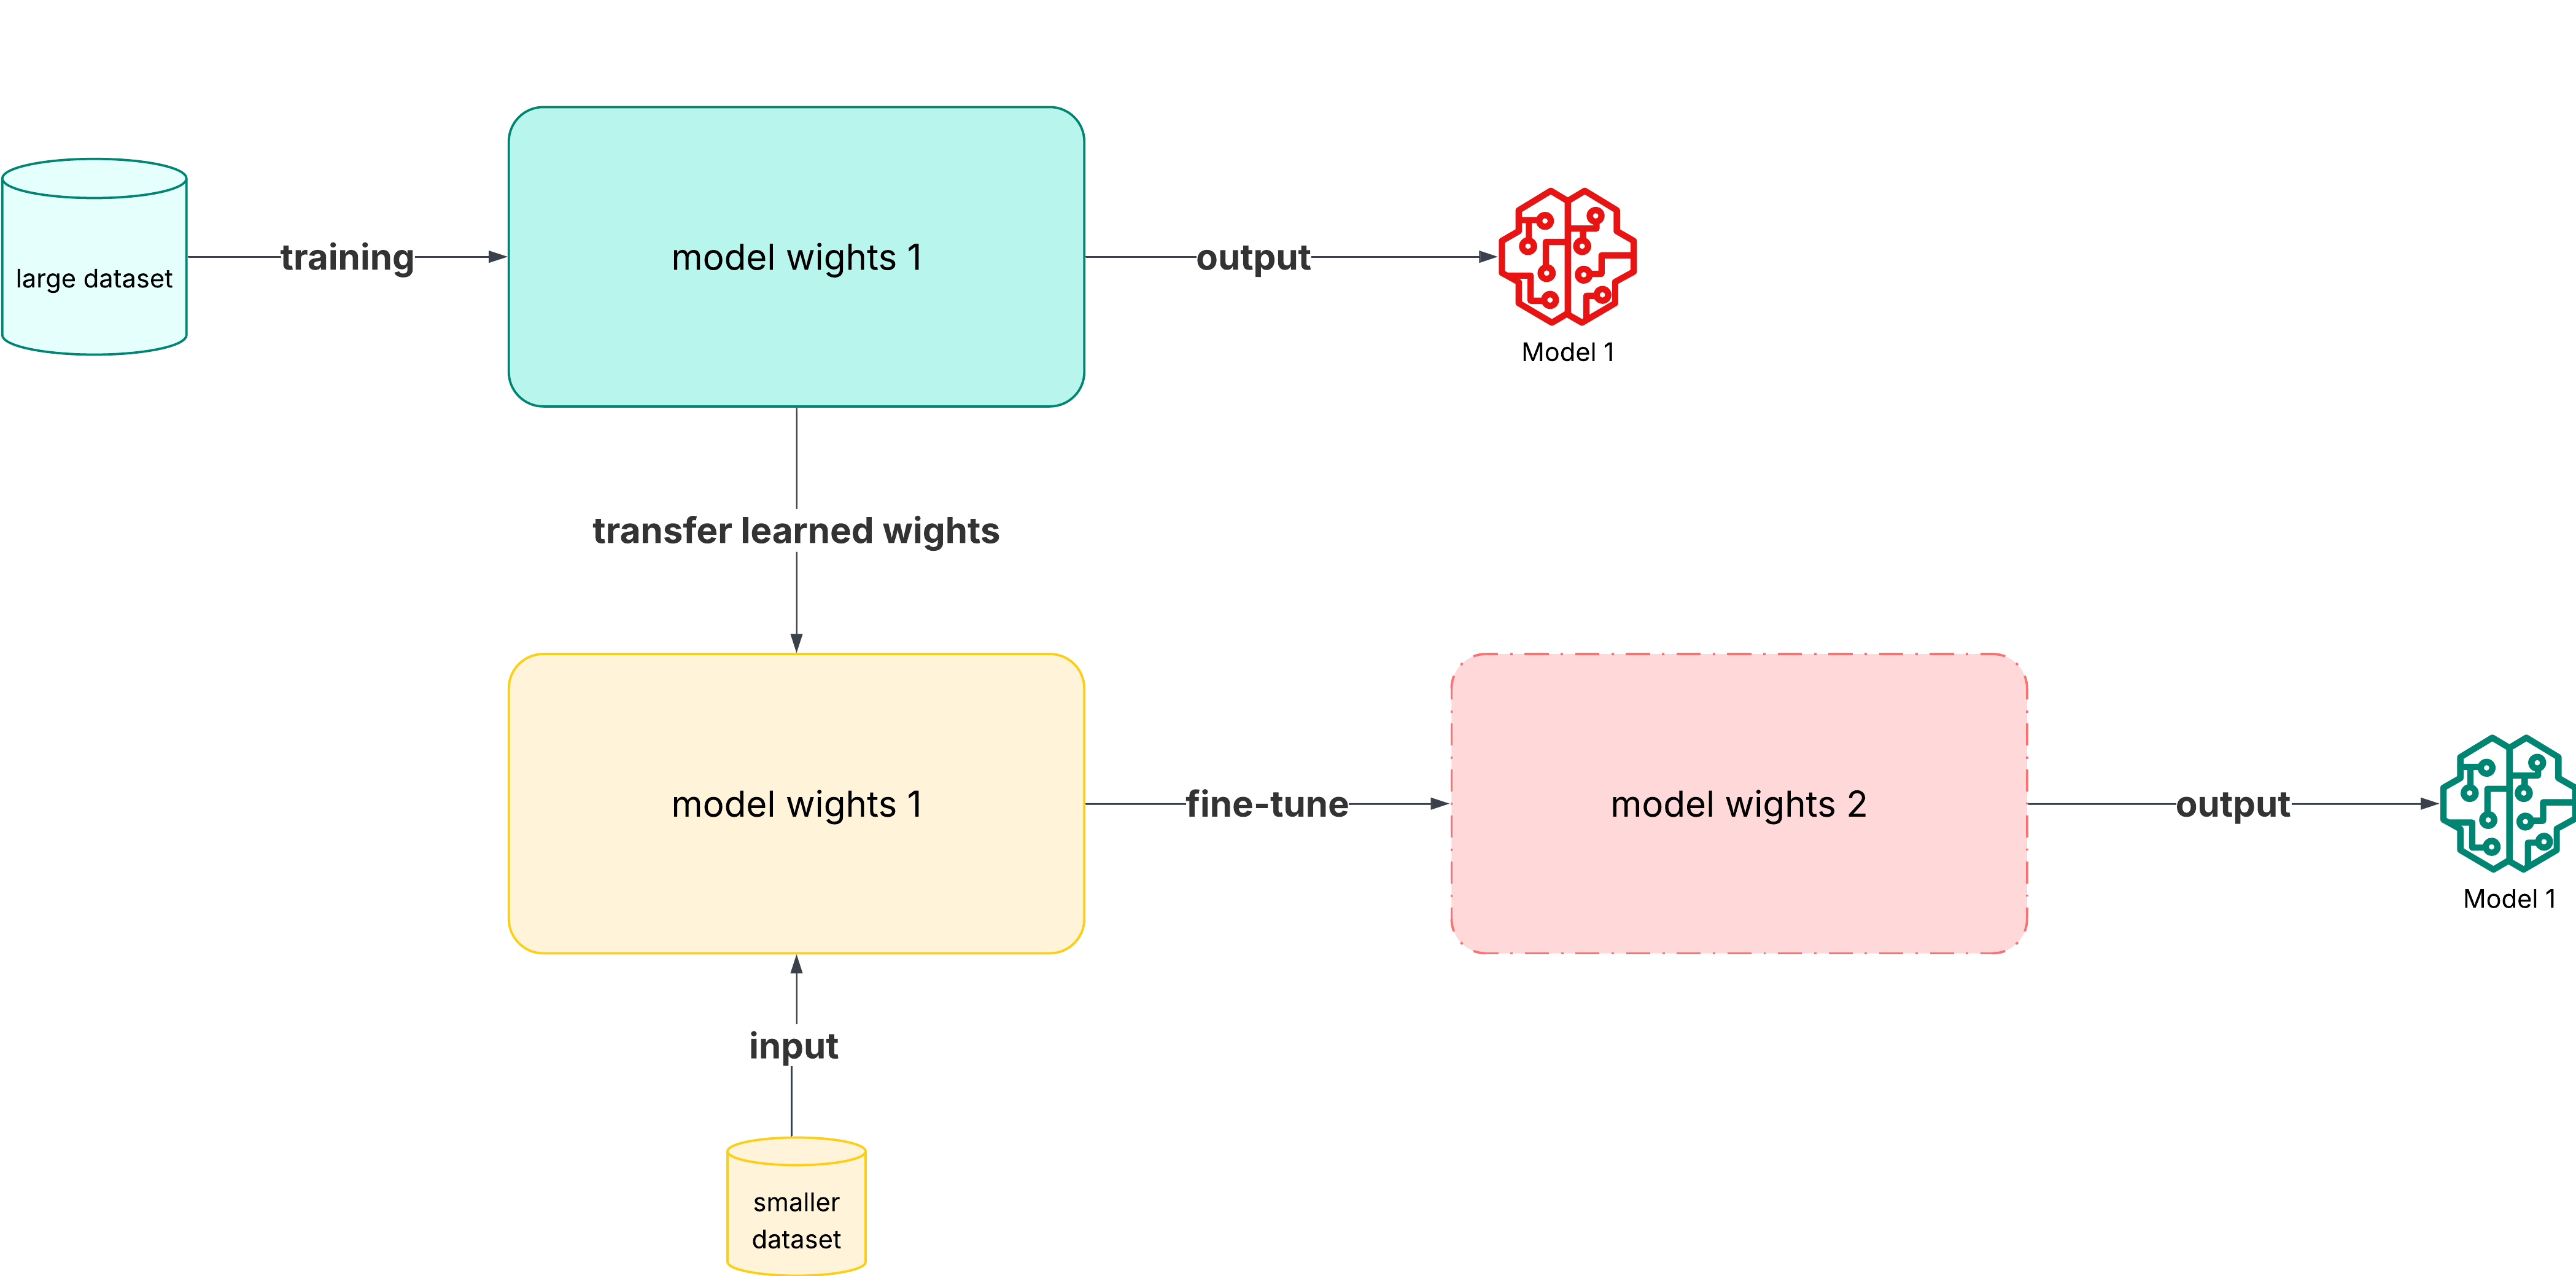
\includegraphics[width=0.7\textwidth]{Transfer_pipeline.png}
  \caption{Schematic exmple of transfer learning pipeline.}
  \label{fig:menegola-pipeline}
\end{figure}

\subsection{EfficientNet Ensemble Approach (Ha et al., 2020)}
To address the challenges of melanoma classification, Ha et al. \cite{ha2020efficientnet} proposed an ensemble approach based on the EfficientNet architecture. Their method incorporates patient metadata, such as age and sex, to improve the accuracy of melanoma detection. By combining multiple EfficientNet models and leveraging contextual information, their solution achieved state-of-the-art results in the SIIM-ISIC Melanoma Classification Challenge.

\begin{enumerate}
  \item Integration of 9 EfficientNet variants (B0--B8) with varying input sizes.
  \item Use of diagnosis-level labels to refine class definitions.
  \item A two-stage ensemble: model-level averaging followed by meta-classifier stacking.
\end{enumerate}
Their solution achieved a cross-validated AUC of 0.96 on the validation set and 0.94 on the test set, outperforming previous state-of-the-art methods. 


\subsection{Contextual Data Augmentation (DiSanto et al., 2022)}
DiSanto et al. \cite{disanto2022contextual} focused on improving the generalization capabilities of melanoma detection models by leveraging contextual data augmentation. They developed a custom data augmentation pipeline that generates realistic skin lesion images with diverse contextual variations. Their approach aims to enhance the robustness of melanoma classifiers by exposing them to a wider range of imaging conditions and reducing overfitting to specific datasets.

\begin{itemize}
  \item Scale jittering to simulate different camera distances.
  \item Random brightness and contrast adjustments for lighting conditions.
  \item Geometric transformations (rotation, perspective warp) to mimic framing differences.
\end{itemize}
They observed a relative increase of 5--7\% in out-of-distribution AUC compared to standard augmentations. Table~\ref{tab:disanto-results} details their comparative study.

\begin{table}[h!]
  \centering
  \caption{Augmentation strategies and performance (DiSanto et al., 2022)}
  \label{tab:disanto-results}
  \begin{tabular}{lcc}
    \hline
    Augmentation set & In-domain AUC & Out-of-domain AUC \\
    \hline
    Standard flips & 0.93 & 0.85 \\
    Contextual pipeline & 0.94 & 0.91 \\
    \hline
  \end{tabular}
\end{table}

\begin{figure}[ht]
  \centering
  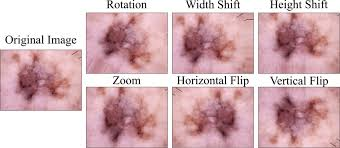
\includegraphics[width=0.5\textwidth]{download.jpg}
  \caption{Examples of image augmentation in skin cancer.}
  \label{fig:disanto-aug}
\end{figure}

\section{mixture of experts}
Mixture of Experts (MoE) is an ensemble strategy that combines multiple specialized sub-models, or "experts," each handling different parts of the input space. A gating network directs each input to one or more experts, allowing the overall model to scale capacity efficiently and focus computation only where needed.

\subsection{Switch Transformer (Fedus et al., 2021)}
\textcite{fedus2021switch} introduced the Switch Transformer, a sparse MoE model for NLP that activates only one expert per token, reducing computational cost while retaining model capacity. Their architecture replaces dense feed-forward layers with MoE layers comprising hundreds of experts and employs a lightweight routing mechanism. To address training instability and communication overhead, they utilize reduced-precision (bfloat16) training and a simplified gating algorithm with dropout safeguarding underutilized experts. The Switch Transformer demonstrates up to 1.8$\times$ speedup in pre-training and strong cross-lingual transfer performance on multilingual benchmarks, scaling to models with over one trillion parameters.

\begin{table}[h!]
  \centering
  \caption{Switch Transformer performance and scaling results (Fedus et al., 2021)}
  \label{tab:switch-transformer}
  \begin{tabular}{lcc}
    \hline
    Model size & Pre-training speedup & Multilingual BLEU \\
    \hline
    200M & 1.2$\times$ & 35.4 \\
    1B & 1.5$\times$ & 37.8 \\
    1T & 1.8$\times$ & 39.2 \\
    \hline
  \end{tabular}
\end{table}

\begin{figure}[H]
  \centering
  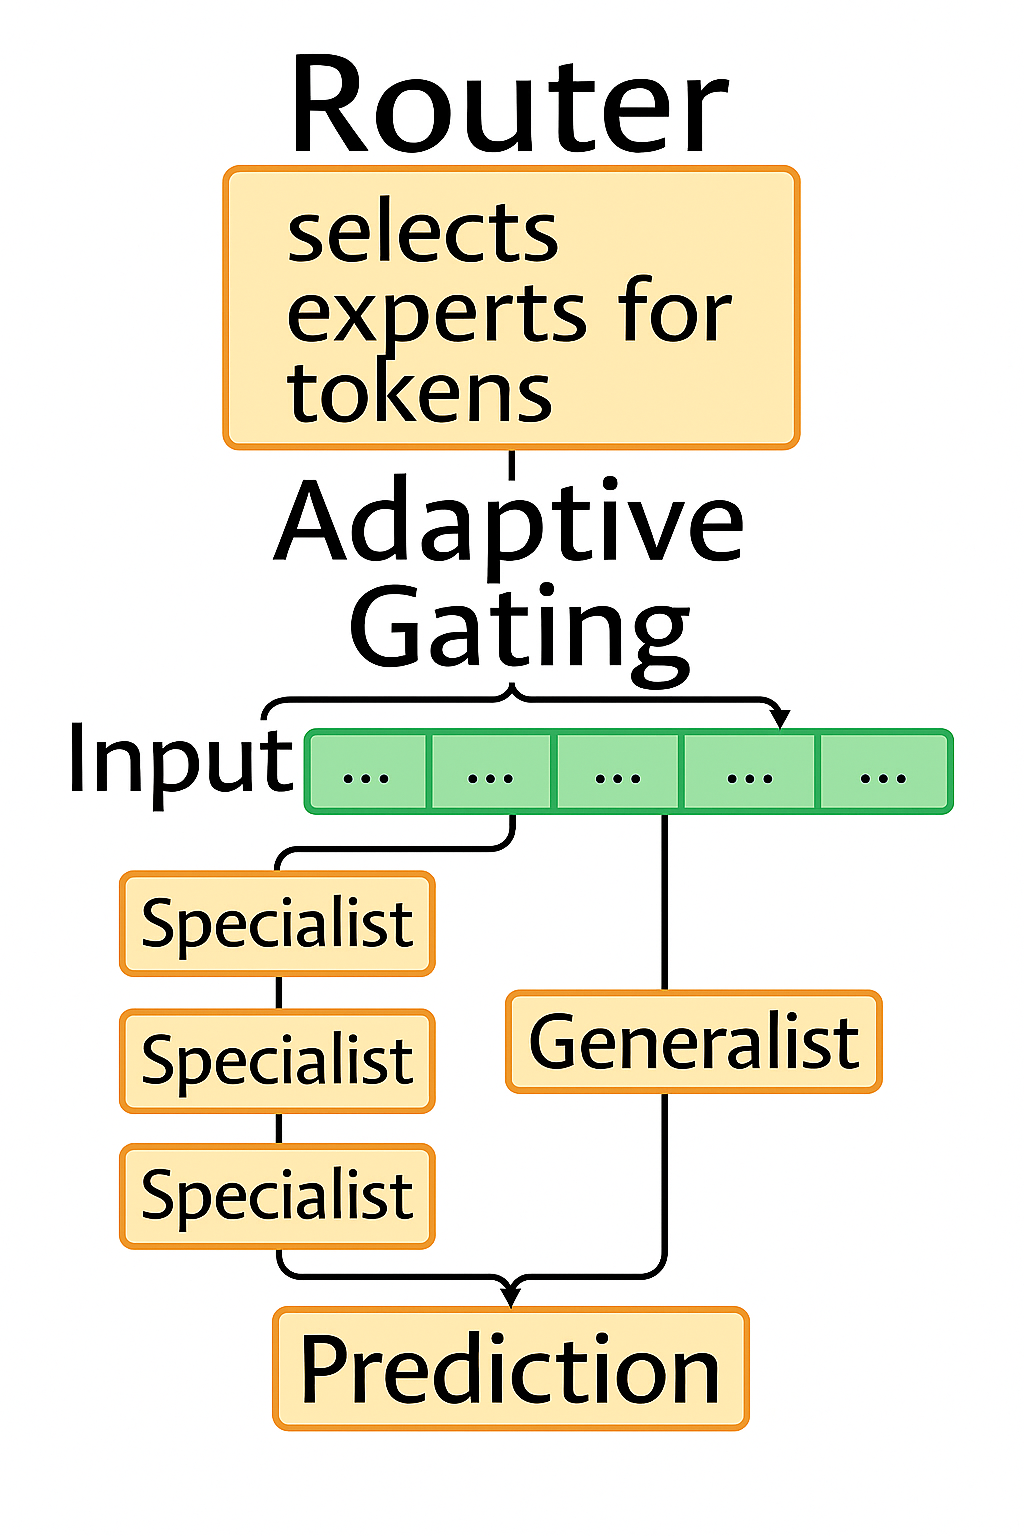
\includegraphics[width=0.5\textwidth]{switch.png}
  \caption{diagram of a switch MOE.}
  \label{fig:switch-transformer}
\end{figure}

\subsection{Vision Mixture of Experts (Riquelme et al., 2021)}
\textcite{riquelme2021scaling} extended sparse MoE to computer vision by integrating MoE feed-forward layers into Vision Transformers, creating the V-MoE model. They introduce an adaptive routing strategy that allocates more experts to complex inputs and fewer to simpler ones, enabling dynamic computational budgets. Trained on ImageNet-21k and fine-tuned on ImageNet, V-MoE achieves comparable or better top-1 accuracy than dense ViTs while using 30\% less FLOPs. The largest variant with 15B parameters attains over 90\% top-1 accuracy on ImageNet.

\begin{table}[h!]
  \centering
  \caption{V-MoE accuracy and efficiency comparison (Riquelme et al., 2021)}
  \label{tab:vmoe-results}
  \begin{tabular}{lccc}
    \hline
    Model size & Params & ImageNet top-1 & FLOPs ($\times10^9$) \\
    \hline
    ViT-B/16 & 86M & 0.779 & 55 \\
    V-MoE-B/16 & 86M+Experts & 0.792 & 38 \\
    V-MoE-L/16 & 15B & 0.903 & 85 \\
    \hline
  \end{tabular}
\end{table}

\begin{figure}[ht]
  \centering
  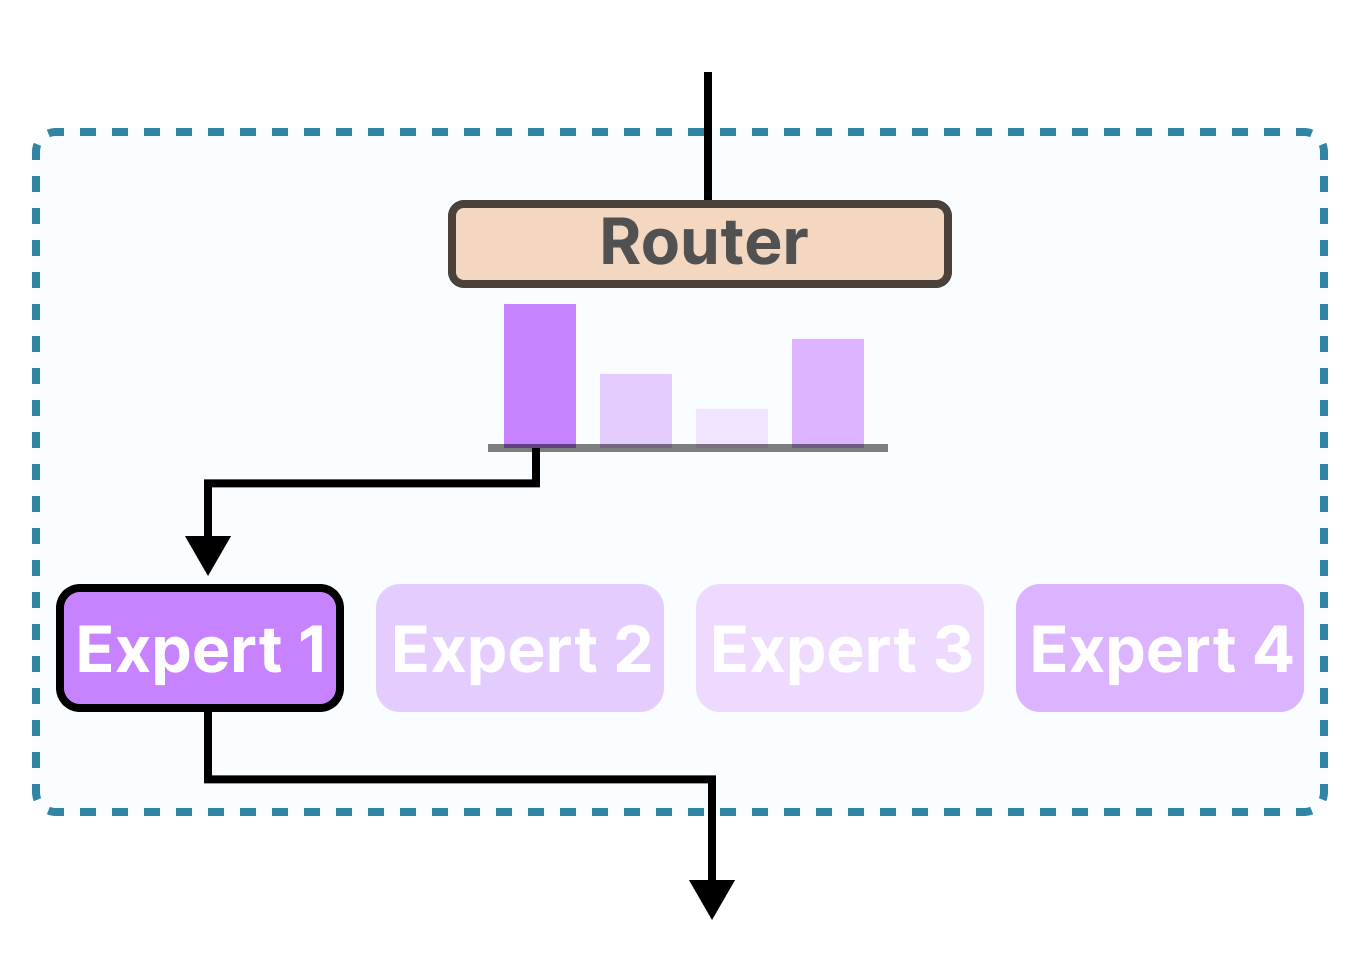
\includegraphics[width=0.7\textwidth]{vmoe.png}
  \caption{Adaptive expert routing in Vision Mixture of Experts.}
  \label{fig:vmoe-routing}
\end{figure}

\section{Conclusion}

This chapter reviewed key advancements in automated skin cancer detection and explored the integration of Mixture of Experts (MoE) models across domains. In the domain of skin cancer detection, several strategies have demonstrated notable improvements in classification performance. Menegola et al. (2017) showed that transfer learning protocols, especially multi-step transfer, significantly improve AUC scores when fine-tuning CNNs for melanoma detection. Ha et al. (2020) introduced an ensemble of EfficientNet models, enhanced with patient metadata and meta-classification, which achieved near state-of-the-art AUCs on both validation and test sets. DiSanto et al. (2022) demonstrated that advanced contextual augmentations yield more robust generalization, particularly on out-of-distribution data.

In the Mixture of Experts domain, Fedus et al. (2021) presented the Switch Transformer for NLP tasks, achieving substantial speedups and scalability through sparse expert activation. Riquelme et al. (2021) extended MoE strategies to vision models with V-MoE, demonstrating adaptive expert routing that improved accuracy while reducing computational cost.

Together, these findings highlight the promise of combining CNN-based backbone  and the potential of MoE architectures for scalable, adaptive learning. In this work, we aim to explore MoE approaches tailored to the dermatology domain, particularly for melanoma classification, with the goal of achieving high diagnostic performance and improved generalization on  dermoscopic datasets.
\chapter{Étude de l'existant}
\clearpage
\label{sec:organisme}

\section{Introduction}
Lorem ipsum dolor sit amet, consectetur adipiscing elit. Proin posuere euismod neque, non semper nibh viverra sed. Praesent ut varius magna. Fusce ipsum ante, semper nec interdum at, semper et lacus. Nulla ultrices magna a fringilla finibus. Etiam sollicitudin blandit ante. Vivamus blandit rhoncus tincidunt. Morbi sit amet congue purus. Praesent interdum gravida congue. Donec fermentum dui fermentum maximus rutrum.


\section{Présentation de l’organisme d’accueil}
Djezzy Lorem ipsum dolor sit amet, consectetur adipiscing elit. Proin posuere euismod neque, non semper nibh viverra sed. Praesent ut varius magna. Fusce ipsum ante, semper nec interdum at, semper et lacus. Nulla ultrices magna a fringilla finibus. Etiam sollicitudin blandit ante. Vivamus blandit rhoncus tincidunt. Morbi sit amet congue purus. Praesent interdum gravida congue. Donec fermentum dui fermentum maximus rutrum.

\medskip

Djezzy couvre 95 \% de Lorem ipsum dolor sit amet, consectetur adipiscing elit. Proin posuere euismod neque, non semper nibh viverra sed. Praesent ut varius magna. Fusce ipsum ante, semper nec interdum at, semper et lacus. Nulla ultrices magna a fringilla finibus. Etiam sollicitudin blandit ante. Vivamus blandit rhoncus tincidunt. Morbi sit amet congue purus. Praesent interdum gravida congue. Donec fermentum dui fermentum maximus rutrum., le 1\textsuperscript{er} octobre 2016, dans 20 wilayasLorem ipsum dolor sit amet, consectetur adipiscing elit. Proin posuere euismod neque, non semper nibh viverra sed. Praesent ut varius magna. Fusce ipsum ante, semper nec interdum at, semper et lacus. Nulla ultrices magna a fringilla finibus. Etiam sollicitudin blandit ante. Vivamus blandit rhoncus tincidunt. Morbi sit amet congue purus. Praesent interdum gravida congue. Donec fermentum dui fermentum maximus rutrum..

\medskip

Lorem ipsum dolor sit amet, consectetur adipiscing elit. Proin posuere euismod neque, non semper nibh viverra sed. Praesent ut varius magna. Fusce ipsum ante, semper nec interdum at, semper et lacus. Nulla ultrices magna a fringilla finibus. Etiam sollicitudin blandit ante. Vivamus blandit rhoncus tincidunt. Morbi sit amet congue purus. Praesent interdum gravida congue. Donec fermentum dui fermentum maximus rutrum. L’entreprise est dirigée par \textit{Matthieu Galvani}, Directeur Général.

\medskip

Lorem ipsum dolor sit amet, consectetur adipiscing elit. Proin posuere euismod neque, non semper nibh viverra sed. Praesent ut varius magna. Fusce ipsum ante, semper nec interdum at, semper et lacus. Nulla ultrices magna a fringilla finibus. Etiam sollicitudin blandit ante. Vivamus blandit rhoncus tincidunt. Morbi sit amet congue purus. Praesent interdum gravida congue. Donec fermentum dui fermentum maximus rutrum. \parencite{djezzy_propos_2019}.

Dates clés de Djezzy GSM :
\begin{itemize}
  \item  Octroi de la licence 2G : 30 juillet 2001
  \item  Octroi de la licence 3G : 2 décembre 2013
  \item  Octroi de la licence 4G : 4 septembre 2016
\end{itemize}


\begin{figure}[hbt!]
  \centering
  
\includegraphics[width=5cm]{Logo_Djezzy_2015}
  \caption{Logo de Djezzy.}
  \label{fig:logo-djezzy}
\end{figure}
\FloatBarrier

\subsection{VEON}
Lorem ipsum dolor sit amet, consectetur adipiscing elit. Proin posuere euismod neque, non semper nibh viverra sed. Praesent ut varius magna. Fusce ipsum ante, semper nec interdum at, semper et lacus. Nulla ultrices magna a fringilla finibus. Etiam sollicitudin blandit ante. Vivamus blandit rhoncus tincidunt. Morbi sit amet congue purus. Praesent interdum gravida congue. Donec fermentum dui fermentum maximus rutrum.Lorem ipsum dolor sit amet, consectetur adipiscing elit. Proin posuere euismod neque, non semper nibh viverra sed. Praesent ut varius magna. Fusce ipsum ante, semper nec interdum at, semper et lacus. Nulla ultrices magna a fringilla finibus. Etiam sollicitudin blandit ante. Vivamus blandit rhoncus tincidunt. Morbi sit amet congue purus. Praesent interdum gravida congue. Donec fermentum dui fermentum maximus rutrum.\parencite{djezzy_propos_2019}.

\begin{figure}[hbt!]
  \centering
  
\includegraphics[width=5cm]{Veon_logo17}
  \caption{Logo de VEON.}
  \label{fig:logo-veon}
\end{figure}
\FloatBarrier

\medskip

\subsection{Vision de Djezzy}
Lorem ipsum dolor sit amet, consectetur adipiscing elit. Proin posuere euismod neque, non semper nibh viverra sed. Praesent ut varius magna. Fusce ipsum ante, semper nec interdum at, semper et lacus. Nulla ultrices magna a fringilla finibus. Etiam sollicitudin blandit ante. Vivamus blandit rhoncus tincidunt. Morbi sit amet congue purus. Praesent interdum gravida congue. Donec fermentum dui fermentum maximus rutrum. \parencite{djezzy_vision_2019}.

\medskip

\subsection{Missions de Djezzy}
Pour réaliser sa vision, Djezzy s'engage à :
\begin{itemize}
  \item  Offrir les meilleurs produits, de qualité, à des prix compétitifs.
  \item  Déployer des infrastructures à la pointe de la technologie.
  \item  Créer pour ses employés le meilleur environnement de travail et d’épanouissement.
  \item Contribuer activement au bien-être des Algériens.
  \item Optimiser la création de valeur pour ses actionnaires, à travers un contrôle strict des coûts.
  \item Appliquer rigoureusement sa politique environnementale.
  \item Améliorer sans cesse ses processus internes dans le respect de sa politique qualité \parencite{djezzy_vision_2019}.
\end{itemize}

\medskip

\subsection{Transformation digitale}
Lorem ipsum dolor sit amet, consectetur adipiscing elit. Proin posuere euismod neque, non semper nibh viverra sed. Praesent ut varius magna. Fusce ipsum ante, semper nec interdum at, semper et lacus. Nulla ultrices magna a fringilla finibus. Etiam sollicitudin blandit ante. Vivamus blandit rhoncus tincidunt. Morbi sit amet congue purus. Praesent interdum gravida congue. Donec fermentum dui fermentum maximus rutrum. \parencite{dabi-schwebel_transformation_2019}. Lorem ipsum dolor sit amet, consectetur adipiscing elit. Proin posuere euismod neque, non semper nibh viverra sed. Praesent ut varius magna. Fusce ipsum ante, semper nec interdum at, semper et lacus. Nulla ultrices magna a fringilla finibus. Etiam sollicitudin blandit ante. Vivamus blandit rhoncus tincidunt. Morbi sit amet congue purus. Praesent interdum gravida congue. Donec fermentum dui fermentum maximus rutrum. :
\begin{itemize}
    \item Rationaliser les ressources (humaines et matérielles ) en centralisant les systèmes d'informations et informatiques.
    \item Réduire les coûts en sous-traitant certains services techniques.
    \item Se positionner dans le monde du digital en proposant de nouveaux services.
    \item Exploiter les opportunités offertes par les nouvelles technologies telles que le Big Data.
    \item Mettre ses employés dans les meilleures conditions de travail pour améliorer la productivité.
\end{itemize}

\medskip


\subsection{Département d'accueil: Service Big Data}
Lorem ipsum dolor sit amet, consectetur adipiscing elit. Proin posuere euismod neque, non semper nibh viverra sed. Praesent ut varius magna. Fusce ipsum ante, semper nec interdum at, semper et lacus. Nulla ultrices magna a fringilla finibus. Etiam sollicitudin blandit ante. Vivamus blandit rhoncus tincidunt. Morbi sit amet congue purus. Praesent interdum gravida congue. Donec fermentum dui fermentum maximus rutrum. :
\begin{itemize}
    \item Permettre à l'entreprise de réagir en temps réel face aux différents changements.
    \item Aider l'entreprise à mieux cibler les clients en répondant à des cas d'utilisation très spécifiques.
    \item Réduire les coûts en exploitant les avantages des technologies Big Data.
    \item Aider les responsables à prendre les décisions adéquates en fournissant les données et les analyses nécessaires.
\end{itemize}

\section{Étude de l'existant}
\label{sec:existant}
Lorem ipsum dolor sit amet, consectetur adipiscing elit. Proin posuere euismod neque, non semper nibh viverra sed. Praesent ut varius magna. Fusce ipsum ante, semper nec interdum at, semper et lacus. Nulla ultrices magna a fringilla finibus. Etiam sollicitudin blandit ante. Vivamus blandit rhoncus tincidunt. Morbi sit amet congue purus. Praesent interdum gravida congue. Donec fermentum dui fermentum maximus rutrum.

\subsection{Recueil d'informations}
Lorem ipsum dolor sit amet, consectetur adipiscing elit. Proin posuere euismod neque, non semper nibh viverra sed. Praesent ut varius magna. Fusce ipsum ante, semper nec interdum at, semper et lacus. Nulla ultrices magna a fringilla finibus. Etiam sollicitudin blandit ante. Vivamus blandit rhoncus tincidunt. Morbi sit amet congue purus. Praesent interdum gravida congue. Donec fermentum dui fermentum maximus rutrum.

\medskip


\begin{xltabular}{\linewidth}{|c|c|c|c|X|}
    \hline
    Num & Date & Type & Service & Points abordés     \\\hline
    1 &  04/11/2019 & Sortie sur terrain & Commercial & Travail de l'animateur  \\[5ex]\hline
    2 &  07/11/2019 & Réunion & Commercial & Explication de la méthode de travail des animateurs  \\\hline
    3 &  07/11/2019 & Réunion & Big Data & Présentation de l’installation technologique de l’entreprise  \\\hline
    4 &  13/11/2019 & Réunion & Commercial & Discussion sur les points de vente  \\\hline
    5 &  25/11/2019 & Réunion & Big Data & Discussion sur l’architecture Big Data de Djezzy  \\\hline
    6 &  27/11/2019 & Réunion & Big Data & Explication de l’architecture globale de Djezzy  \\\hline
    7 &  04/12/2019 & Réunion & Data science & Discussion sur les KPIs pertinents relatifs aux points de vente  \\\hline
    8 &  08/12/2019 & Réunion & Commercial & Discussion sur l’organisation des régions.  \\\hline
    9 &  09/12/2019 & Réunion & Reporting & Discussion sur le reporting des points de vente  \\\hline
    
   
    \caption{L'ensemble des réunions et sorties réalisées.}
    \label{tab:meetings}
\end{xltabular}
\FloatBarrier


\subsection{Réseau de distribution de Djezzy}

Lorem ipsum dolor sit amet, consectetur adipiscing elit. Proin posuere euismod neque, non semper nibh viverra sed. Praesent ut varius magna. Fusce ipsum ante, semper nec interdum at, semper et lacus. Nulla ultrices magna a fringilla finibus. Etiam sollicitudin blandit ante. Vivamus blandit rhoncus tincidunt. Morbi sit amet congue purus. Praesent interdum gravida congue. Donec fermentum dui fermentum maximus rutrum.

\medskip

\begin{figure}[hbt!]
  \centering
  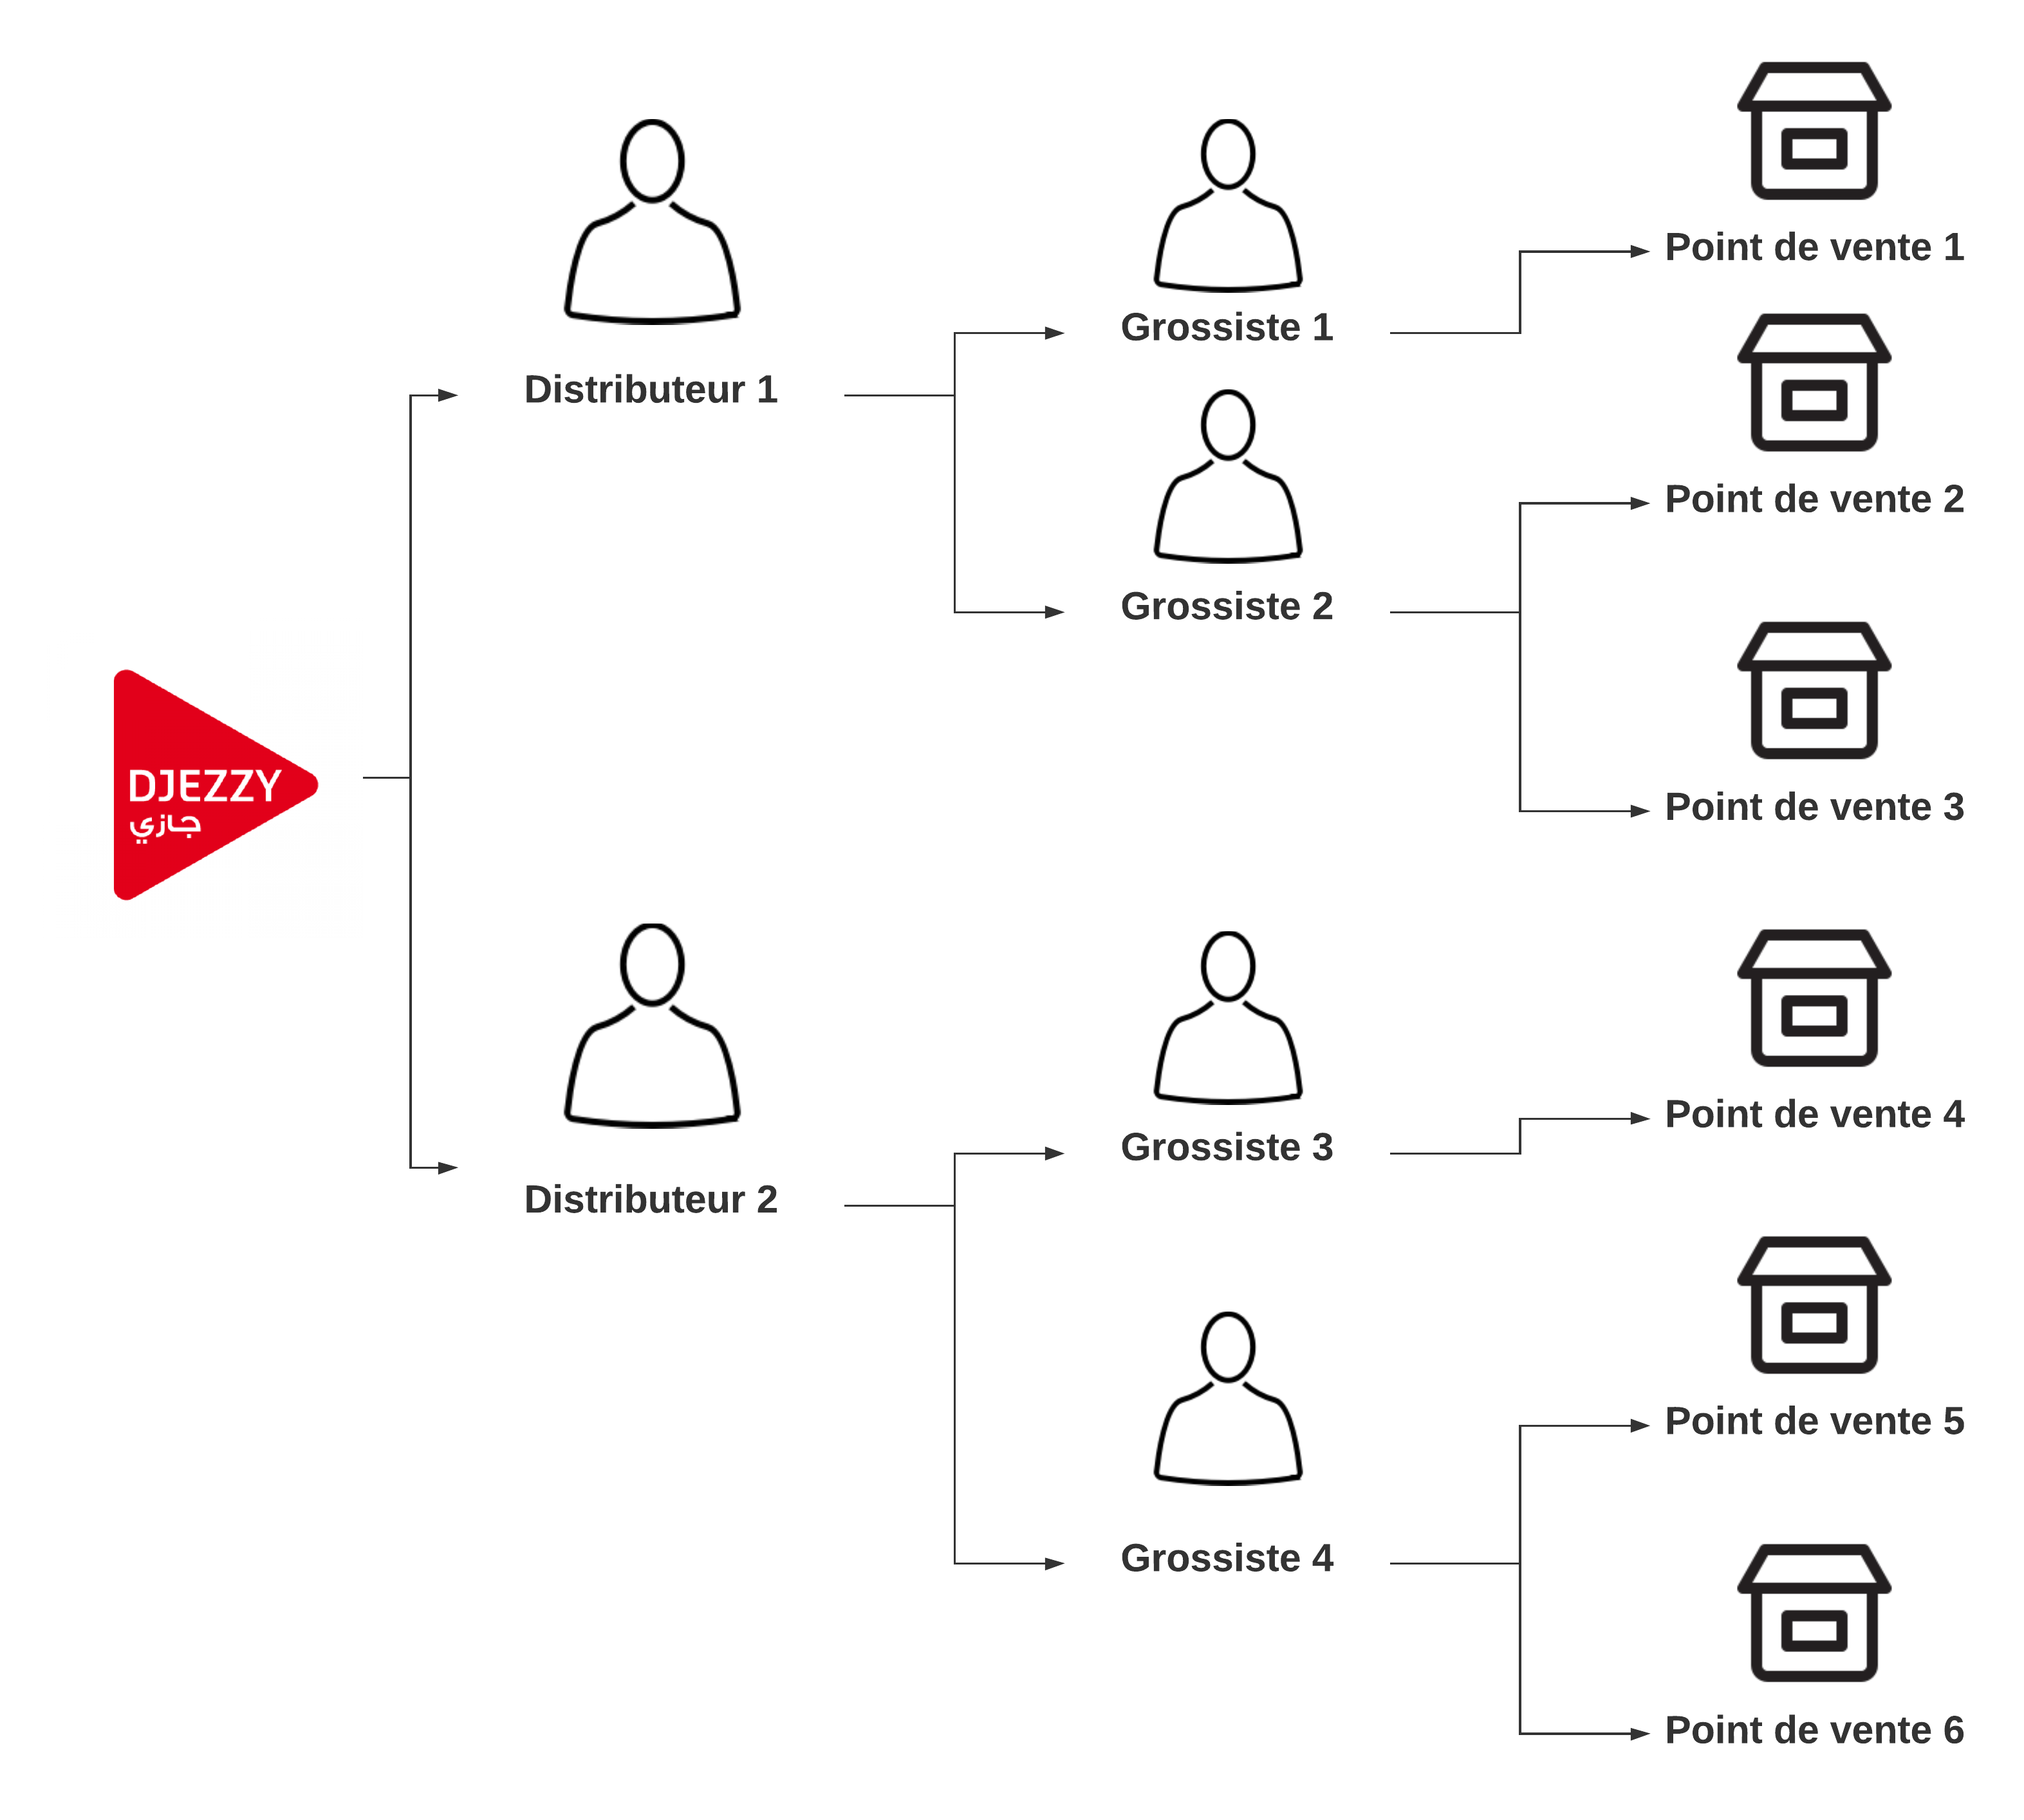
\includegraphics[width=14cm]{images_pfe/reseau_distribution.png}
  \caption{Réseau de distribution de Djezzy.}
  \label{fig:reseau-distribution}
\end{figure}
\FloatBarrier

Lorem ipsum dolor sit amet, consectetur adipiscing elit. Proin posuere euismod neque, non semper nibh viverra sed. Praesent ut varius magna. Fusce ipsum ante, semper nec interdum at, semper et lacus. Nulla ultrices magna a fringilla finibus. Etiam sollicitudin blandit ante. Vivamus blandit rhoncus tincidunt. Morbi sit amet congue purus. Praesent interdum gravida congue. Donec fermentum dui fermentum maximus rutrum.

\medskip

\subsection{Point de vente}
\label{sec:pos}

Lorem ipsum dolor sit amet, consectetur adipiscing elit. Proin posuere euismod neque, non semper nibh viverra sed. Praesent ut varius magna. Fusce ipsum ante, semper nec interdum at, semper et lacus. Nulla ultrices magna a fringilla finibus. Etiam sollicitudin blandit ante. Vivamus blandit rhoncus tincidunt. Morbi sit amet congue purus. Praesent interdum gravida congue. Donec fermentum dui fermentum maximus rutrum.Lorem ipsum dolor sit amet, consectetur adipiscing elit. Proin posuere euismod neque, non semper nibh viverra sed. Praesent ut varius magna. Fusce ipsum ante, semper nec interdum at, semper et lacus. Nulla ultrices magna a fringilla finibus. Etiam sollicitudin blandit ante. Vivamus blandit rhoncus tincidunt. Morbi sit amet congue purus. Praesent interdum gravida congue. Donec fermentum dui fermentum maximus rutrum.

\medskip


\begin{figure}[hbt!]
  \centering
  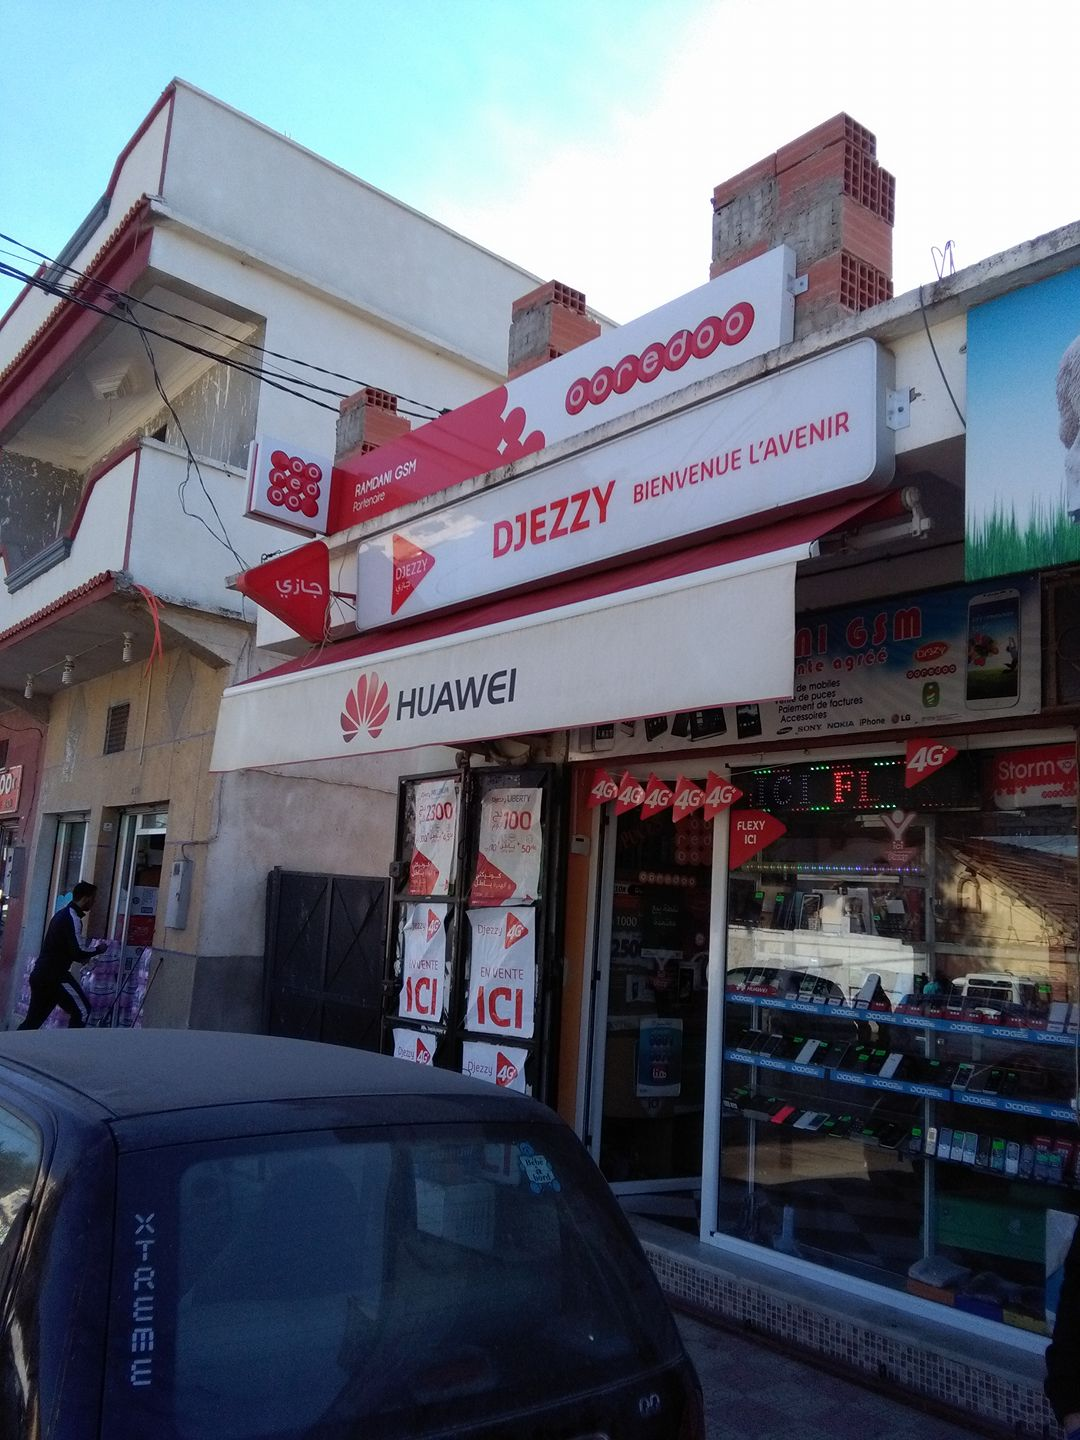
\includegraphics[height=8cm]{images_pfe/point-de-vente.jpg}
  \caption{Un exemple de point de vente Djezzy \parencite{web_image_point_de_vente_2019}.}
  \label{fig:point-de-vente}
\end{figure}
\FloatBarrier

Lorem ipsum dolor sit amet, consectetur adipiscing elit. Proin posuere euismod neque, non semper nibh viverra sed. Praesent ut varius magna. Fusce ipsum ante, semper nec interdum at, semper et lacus. Nulla ultrices magna a fringilla finibus. Etiam sollicitudin blandit ante. Vivamus blandit rhoncus tincidunt. Morbi sit amet congue purus. Praesent interdum gravida congue. Donec fermentum dui fermentum maximus rutrum.Lorem ipsum dolor sit amet, consectetur adipiscing elit. Proin posuere euismod neque, non semper nibh viverra sed. Praesent ut varius magna. Fusce ipsum ante, semper nec interdum at, semper et lacus. Nulla ultrices magna a fringilla finibus. Etiam sollicitudin blandit ante. Vivamus blandit rhoncus tincidunt. Morbi sit amet congue purus. Praesent interdum gravida congue. Donec fermentum dui fermentum maximus rutrum.



\subsection{Animateur de zone}

Lorem ipsum dolor sit amet, consectetur adipiscing elit. Proin posuere euismod neque, non semper nibh viverra sed. Praesent ut varius magna. Fusce ipsum ante, semper nec interdum at, semper et lacus. Nulla ultrices magna a fringilla finibus. Etiam sollicitudin blandit ante. Vivamus blandit rhoncus tincidunt. Morbi sit amet congue purus. Praesent interdum gravida congue. Donec fermentum dui fermentum maximus rutrum.Lorem ipsum dolor sit amet, consectetur adipiscing elit. Proin posuere euismod neque, non semper nibh viverra sed. Praesent ut varius magna. Fusce ipsum ante, semper nec interdum at, semper et lacus. Nulla ultrices magna a fringilla finibus. Etiam sollicitudin blandit ante. Vivamus blandit rhoncus tincidunt. Morbi sit amet congue purus. Praesent interdum gravida congue. Donec fermentum dui fermentum maximus rutrum. :

\medskip

\begin{itemize}
    \item Former et informer les points de vente (produits, offres, challenges, cadeaux...etc.)
    \item Motiver les points de vente pour booster le chiffre d’affaires.
    \item Recueillir et transmettre les informations sur la qualité de réseau, le feedback des clients...etc.
    \item Assurer le marketing (affiches publicitaires, panneau...etc.)
    \item Récupérer les contrats de puces.
    \item Traiter les problèmes des points de vente (activation des puces, Flexy...etc.)
    \item Approbation des nouveaux points de vente.
\end{itemize}

Lorem ipsum dolor sit amet, consectetur adipiscing elit. Proin posuere euismod neque, non semper nibh viverra sed. Praesent ut varius magna. Fusce ipsum ante, semper nec interdum at, semper et lacus. Nulla ultrices magna a fringilla finibus. Etiam sollicitudin blandit ante. Vivamus blandit rhoncus tincidunt. Morbi sit amet congue purus. Praesent interdum gravida congue. Donec fermentum dui fermentum maximus rutrum.Lorem ipsum dolor sit amet, consectetur adipiscing elit. Proin posuere euismod neque, non semper nibh viverra sed. Praesent ut varius magna. Fusce ipsum ante, semper nec interdum at, semper et lacus. Nulla ultrices magna a fringilla finibus. Etiam sollicitudin blandit ante. Vivamus blandit rhoncus tincidunt. Morbi sit amet congue purus. Praesent interdum gravida congue. Donec fermentum dui fermentum maximus rutrum.

\medskip

\begin{figure}[hbt!]
  \centering
  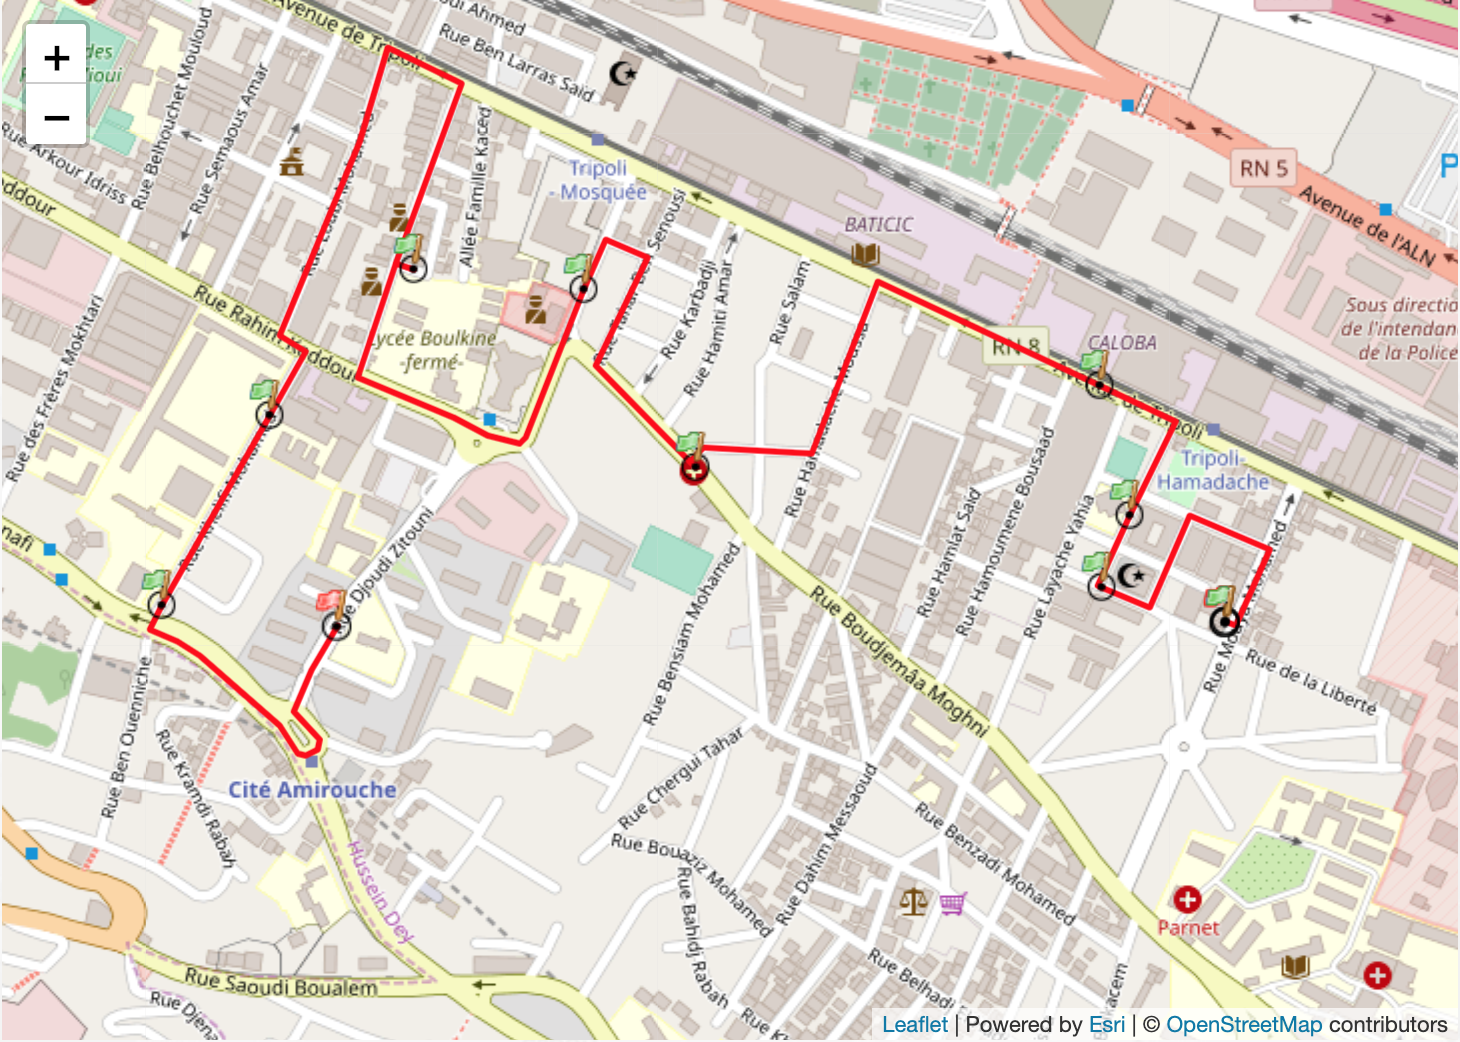
\includegraphics[height=8cm]{images_pfe/animator_route.png}
  \caption{Un exemple de tournée d'un animateur (en rouge).}
  \label{fig:tournee-animateur}
\end{figure}
\FloatBarrier


\medskip

\section{Conclusion}
Lorem ipsum dolor sit amet, consectetur adipiscing elit. Proin posuere euismod neque, non semper nibh viverra sed. Praesent ut varius magna. Fusce ipsum ante, semper nec interdum at, semper et lacus. Nulla ultrices magna a fringilla finibus. Etiam sollicitudin blandit ante. Vivamus blandit rhoncus tincidunt. Morbi sit amet congue purus. Praesent interdum gravida congue. Donec fermentum dui fermentum maximus rutrum.

\medskip

Lorem ipsum dolor sit amet, consectetur adipiscing elit. Proin posuere euismod neque, non semper nibh viverra sed. Praesent ut varius magna. Fusce ipsum ante, semper nec interdum at, semper et lacus. Nulla ultrices magna a fringilla finibus. Etiam sollicitudin blandit ante. Vivamus blandit rhoncus tincidunt. Morbi sit amet congue purus. Praesent interdum gravida congue. Donec fermentum dui fermentum maximus rutrum.






%%% Local Variables: 
%%% mode: latex
%%% TeX-master: "isae-report-template"
%%% End: 
\chapter{Expression des besoins}
\clearpage
\label{chap:besoins}

\section{Introduction}
Lorem ipsum dolor sit amet, consectetur adipiscing elit. Proin posuere euismod neque, non semper nibh viverra sed. Praesent ut varius magna. Fusce ipsum ante, semper nec interdum at, semper et lacus. Nulla ultrices magna a fringilla finibus. Etiam sollicitudin blandit ante. Vivamus blandit rhoncus tincidunt. Morbi sit amet congue purus. Praesent interdum gravida congue. Donec fermentum dui fermentum maximus rutrum.
\section{Définition des utilisateurs}
Lorem ipsum dolor sit amet, consectetur adipiscing elit. Proin posuere euismod neque, non semper nibh viverra sed. Praesent ut varius magna. Fusce ipsum ante, semper nec interdum at, semper et lacus. Nulla ultrices magna a fringilla finibus. Etiam sollicitudin blandit ante. Vivamus blandit rhoncus tincidunt. Morbi sit amet congue purus. Praesent interdum gravida congue. Donec fermentum dui fermentum maximus rutrum.
\subsection{Administrateur}
Lorem ipsum dolor sit amet, consectetur adipiscing elit. Proin posuere euismod neque, non semper nibh viverra sed. Praesent ut varius magna. Fusce ipsum ante, semper nec interdum at, semper et lacus. Nulla ultrices magna a fringilla finibus. Etiam sollicitudin blandit ante. Vivamus blandit rhoncus tincidunt. Morbi sit amet congue purus. Praesent interdum gravida congue. Donec fermentum dui fermentum maximus rutrum.


\subsection{Animateur}
Lorem ipsum dolor sit amet, consectetur adipiscing elit. Proin posuere euismod neque, non semper nibh viverra sed. Praesent ut varius magna. Fusce ipsum ante, semper nec interdum at, semper et lacus. Nulla ultrices magna a fringilla finibus. Etiam sollicitudin blandit ante. Vivamus blandit rhoncus tincidunt. Morbi sit amet congue purus. Praesent interdum gravida congue. Donec fermentum dui fermentum maximus rutrum.

\clearpage

\section{Spécifications}
Lorem ipsum dolor sit amet, consectetur adipiscing elit. Proin posuere euismod neque, non semper nibh viverra sed. Praesent ut varius magna. Fusce ipsum ante, semper nec interdum at, semper et lacus. Nulla ultrices magna a fringilla finibus. Etiam sollicitudin blandit ante. Vivamus blandit rhoncus tincidunt. Morbi sit amet congue purus. Praesent interdum gravida congue. Donec fermentum dui fermentum maximus rutrum.

\subsection{Spécifications fonctionnelles}
Lorem ipsum dolor sit amet, consectetur adipiscing elit. Proin posuere euismod neque, non semper nibh viverra sed. Praesent ut varius magna. Fusce ipsum ante, semper nec interdum at, semper et lacus. Nulla ultrices magna a fringilla finibus. Etiam sollicitudin blandit ante. Vivamus blandit rhoncus tincidunt. Morbi sit amet congue purus. Praesent interdum gravida congue. Donec fermentum dui fermentum maximus rutrum. :
\renewcommand{\arraystretch}{1.5}
\begin{xltabular}{17cm}{|c|X|}
    \hline
    ID & Description     \\\hline
    1 & Le système doit permettre à l'utilisateur (Administrateur, Animateur) de s'authentifier. \\\hline
    2 & Le système doit permettre à l'administrateur de consulter les statistiques des visites des animateurs. \\\hline
    3 & Le système doit permettre à l'administrateur de consulter la liste des animateurs. \\\hline
    4 & Le système doit permettre à l'administrateur de visualiser les points de vente sur la carte. \\\hline
    5 & Le système doit permettre à l'administrateur de générer les plans de visite des animateurs. \\\hline
    6 & Le système doit permettre à l'administrateur de synchroniser les tournées des animateurs en temps réel (selon les fluctuations du trafic routier). \\\hline
    7 & Le système doit permettre à l'administrateur de visualiser les plans de route des animateurs. \\\hline
    8 & Le système doit permettre à l'administrateur de modifier les paramètres de visite des points de vente. \\\hline
    9 & Le système doit permettre à l'administrateur de choisir les types de points de vente à visiter. \\\hline
    10 & Le système doit permettre à l'animateur de récupérer ses plans de visite. \\\hline
    11 & Le système doit permettre à l'animateur de synchroniser ses tournées en temps réel avec les données du trafic routier. \\\hline
    12 & Le système doit permettre à l'animateur de visualiser ses plans de route sur la carte. \\\hline
    13 & Le système doit classifier les points de vente selon leur degré d'importance. \\\hline
    14 & Le système doit mettre à jour la classification des points de vente selon leur rendement mensuel. \\\hline
    15 & Le système doit inclure l'importance des points de vente dans la logique d'élaboration des plans de visite destinés aux animateurs. \\\hline
    
    \caption{L'ensemble des spécifications fonctionnelles.}
    \label{tab:functional-specs}
\end{xltabular}
\FloatBarrier


\subsection{Spécifications techniques}
Lorem ipsum dolor sit amet, consectetur adipiscing elit. Proin posuere euismod neque, non semper nibh viverra sed. Praesent ut varius magna. Fusce ipsum ante, semper nec interdum at, semper et lacus. Nulla ultrices magna a fringilla finibus. Etiam sollicitudin blandit ante. Vivamus blandit rhoncus tincidunt. Morbi sit amet congue purus. Praesent interdum gravida congue. Donec fermentum dui fermentum maximus rutrum. :

\renewcommand{\arraystretch}{1.5}
\begin{xltabular}{17cm}{|c|X|}
    \hline
    ID & Description     \\\hline
    16 & Le système doit être compatible avec l'architecture de données de Djezzy. \\\hline
    17 & L'architecture du système doit être évolutive. \\\hline
    18 & Le système doit générer les plans de visite en un temps réduit (< 10s). \\\hline
    19 & Le système doit être implémenté sous forme d'une solution web. \\\hline
    20 & Les interfaces du système doivent s'adapter à toutes les tailles d'écrans (responsive). \\\hline
    
    
    \caption{L'ensemble des spécifications techniques.}
    \label{tab:technical-specs}
\end{xltabular}
\FloatBarrier

\section{Définition des cas d'utilisation}

Lorem ipsum dolor sit amet, consectetur adipiscing elit. Proin posuere euismod neque, non semper nibh viverra sed. Praesent ut varius magna. Fusce ipsum ante, semper nec interdum at, semper et lacus. Nulla ultrices magna a fringilla finibus. Etiam sollicitudin blandit ante. Vivamus blandit rhoncus tincidunt. Morbi sit amet congue purus. Praesent interdum gravida congue. Donec fermentum dui fermentum maximus rutrum.Lorem ipsum dolor sit amet, consectetur adipiscing elit. Proin posuere euismod neque, non semper nibh viverra sed. Praesent ut varius magna. Fusce ipsum ante, semper nec interdum at, semper et lacus. Nulla ultrices magna a fringilla finibus. Etiam sollicitudin blandit ante. Vivamus blandit rhoncus tincidunt. Morbi sit amet congue purus. Praesent interdum gravida congue. Donec fermentum dui fermentum maximus rutrum.

\clearpage

\subsection{Administrateur}

\begin{figure}[hbt!]
  \centering
  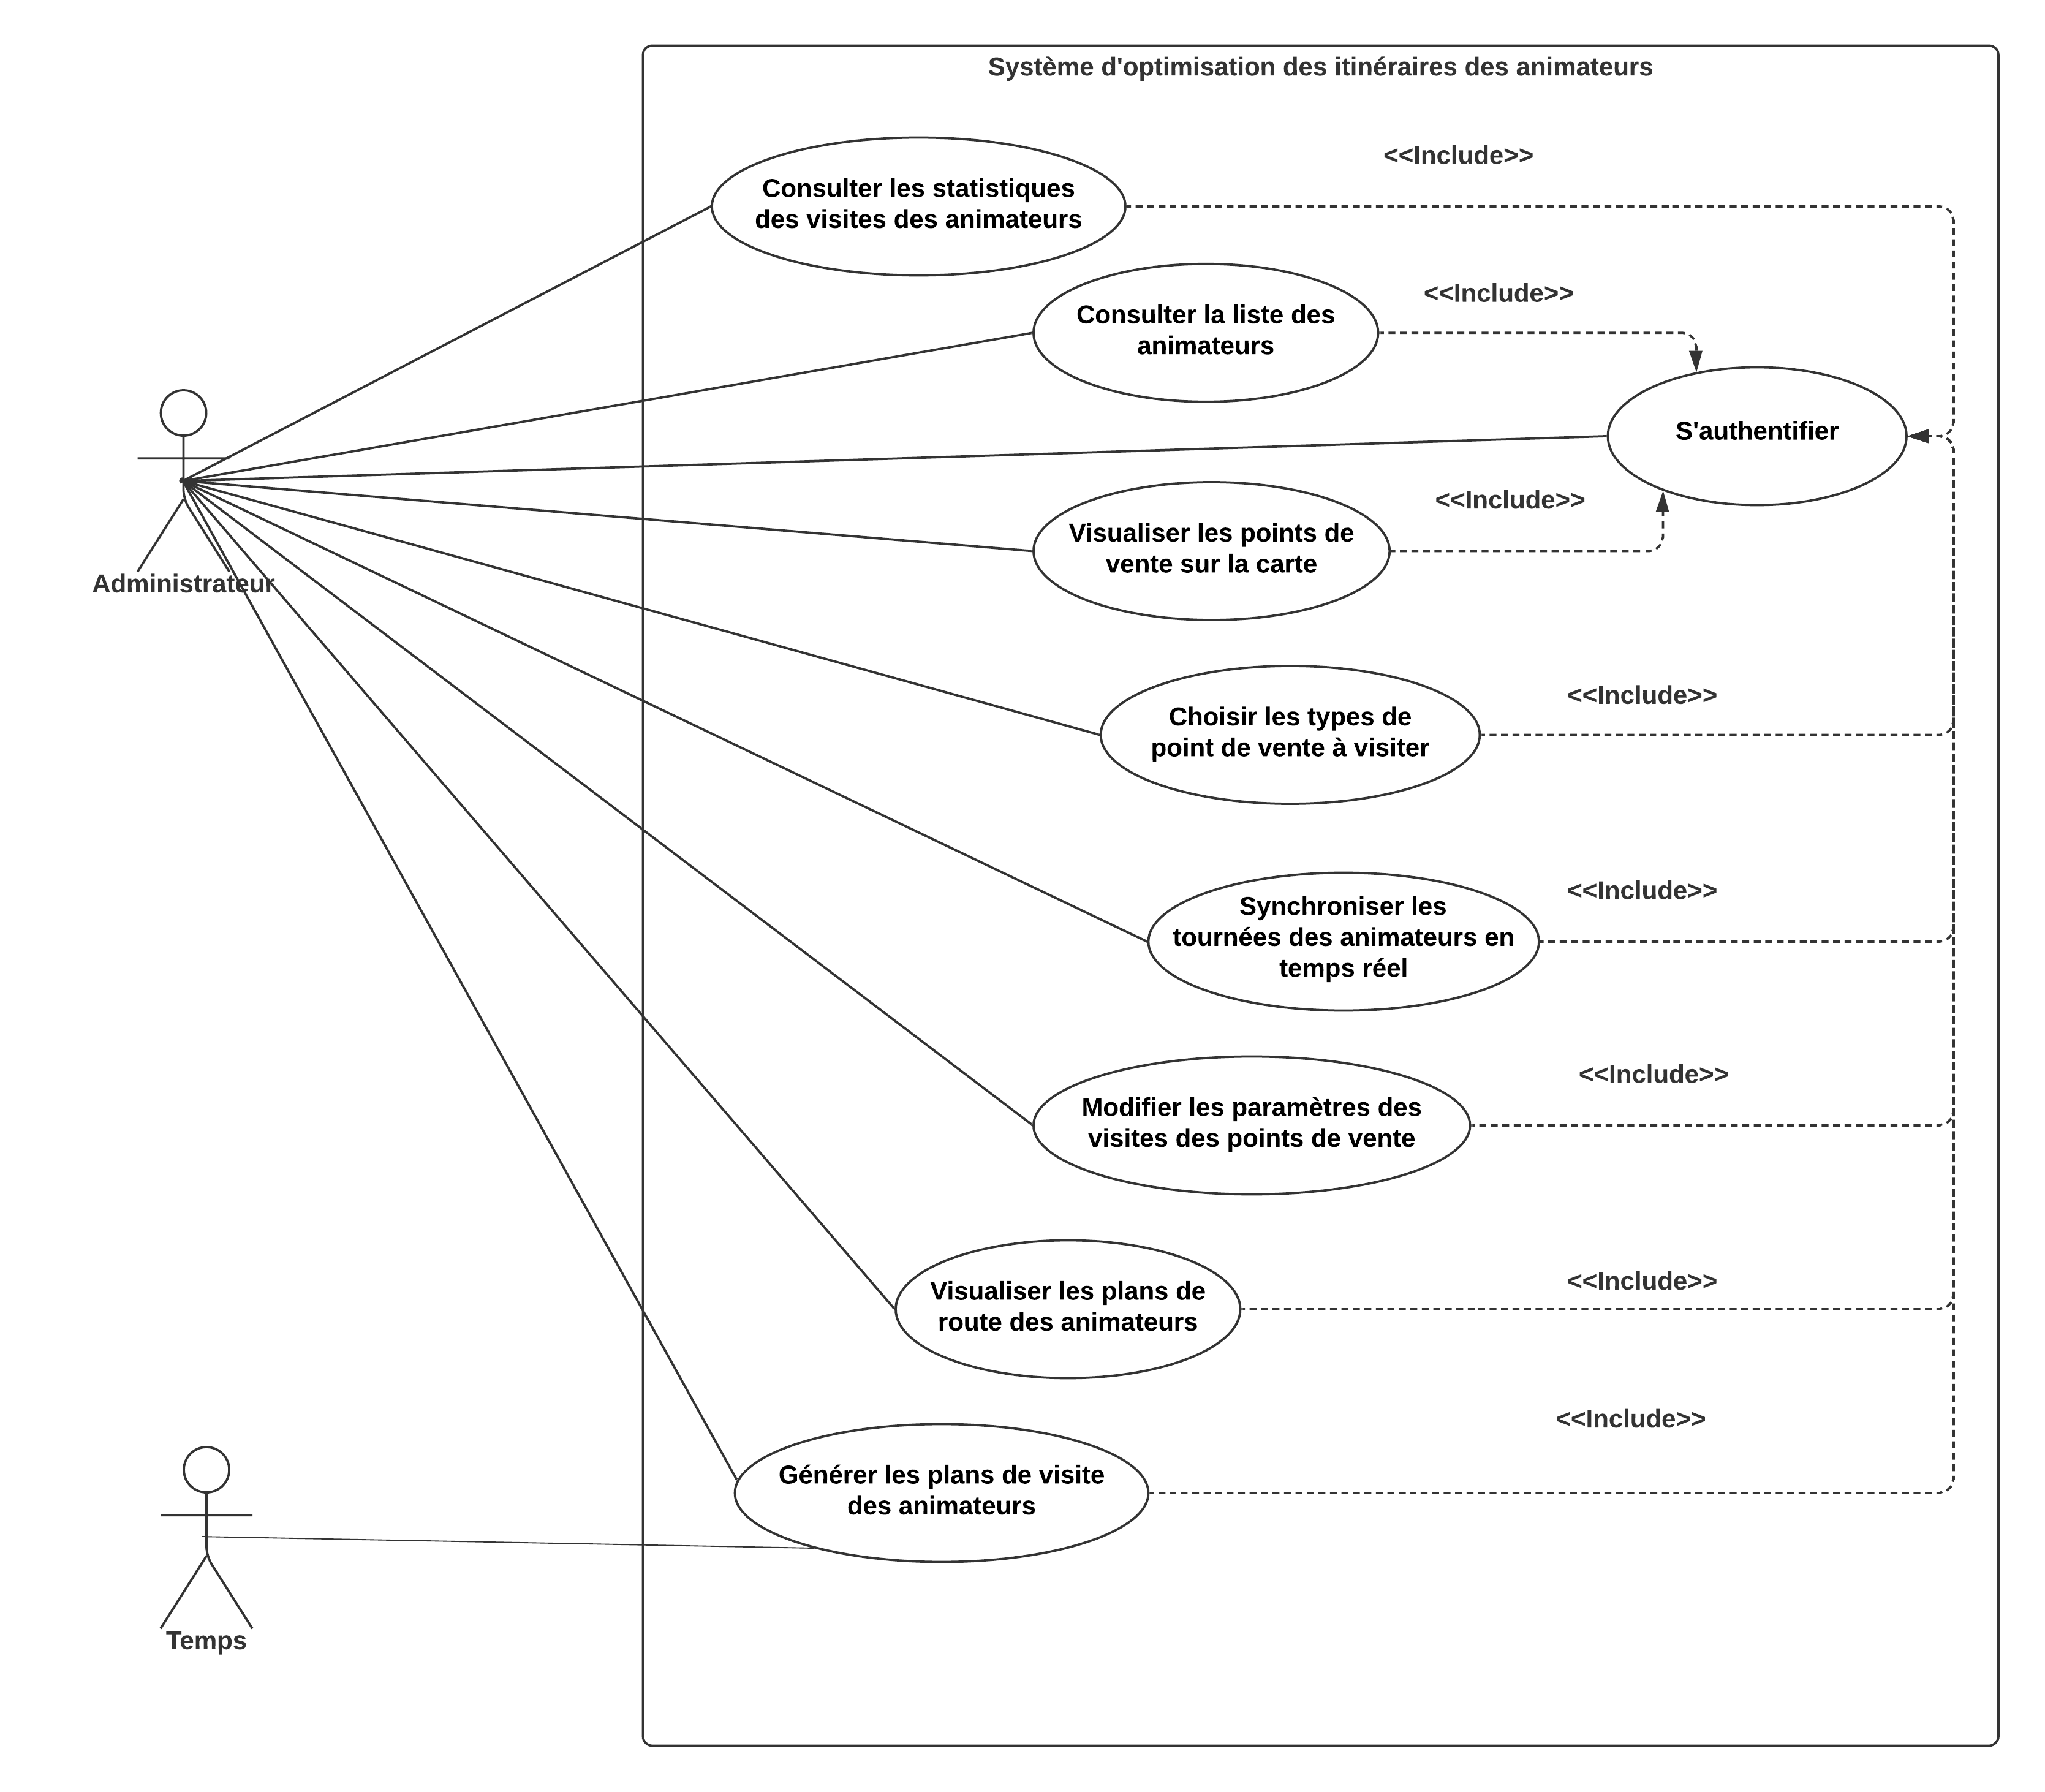
\includegraphics[ width=\linewidth]{images_pfe/DCU_ADMINISTRATEUR.png}
  \caption{Diagramme des cas d'utilisation de l'administrateur.}
  \label{fig:dcu-administrateur}
\end{figure}
\FloatBarrier


\renewcommand{\arraystretch}{1.5}
\begin{xltabular}{\linewidth}{|c|X|c|c|}
    \hline
    ID & CU & Documentation & Diagramme d'activité     \\\hline
    1 & S'authentifier & & \\ \hline
    2 & Consulter les statistiques des visites & & \\ \hline
    3 & Consulter la liste des animateurs & & \\ \hline
    4 & Visualiser les points de vente sur la carte & & \\ \hline
    5 & Générer les plans de visite des animateurs & \checkmark & \checkmark \\ \hline
    6 & Synchroniser les tournées des animateurs & \checkmark &  \\ \hline
    7 & Visualiser les plans de route des animateurs &  &  \\ \hline 
    8 & Modifier les paramètres de visite des points de vente & \checkmark &  \\ \hline
    9 & Choisir les types de points de vente à visiter & & \\ \hline
    \caption{Liste des cas d'utilisation de l'administrateur.}
    \label{tab:admin-use-cases}
\end{xltabular}
\FloatBarrier


\renewcommand{\arraystretch}{1.5}
\begin{xltabular}{\linewidth}{|X|}
    \hline
    \textbf{CU} : Générer les plans de visite des animateurs     \\\hline
    \textbf{ID} :  5   \\\hline
    \textbf{Description brève} : Générer les plans de visite des animateurs avec les chemins optimaux de parcours  \\\hline
    \textbf{Acteurs primaires} : Administrateur, Temps     \\\hline
    \textbf{Acteurs secondaires} :  /    \\\hline
    \textbf{Pré condition} :  l'administrateur déjà connecté    \\\hline
    \textbf{Enchaînement principal} : \\
    Le cas d'utilisation démarre automatiquement de manière périodique, ou lorsque l'administrateur souhaite générer les plans de visite des animateurs. \\
    1. L'administrateur choisit l'onglet génération des plans. \\
    2. Il introduit la période dans laquelle l'animateur va visiter les points de vente (semaine, 15 jours, mois...etc). \\
    3. Il choisit pour chaque type de point de vente sa fréquence de visite pendant la période. \\
    4. Il lance la génération des plans. \\
    5. Le système génère les plans de visite des animateurs. 
    \\\hline
    \textbf{Post condition} :  Les plans de visite sont générés pour l'ensemble des animateurs   \\\hline
    \textbf{Enchaînement alternatif} :   /   \\\hline
  
    \caption{Documentation CU : Générer les plans de visite des animateurs.}
    \label{tab:cu-specs1}
\end{xltabular}
\FloatBarrier

\clearpage

\renewcommand{\arraystretch}{1.5}
\begin{xltabular}{\linewidth}{|X|}
    \hline
    \textbf{CU} : Synchroniser les tournées des animateurs      \\\hline
    \textbf{ID} :  6    \\\hline
    \textbf{Description brève} : Mettre à jour une tournée d'un animateur par rapport à la fluidité du trafic routier     \\\hline
    \textbf{Acteurs primaires} :  Administrateur    \\\hline
    \textbf{Acteurs secondaires} :  /    \\\hline
    \textbf{Pré condition} :  l'administrateur déjà connecté   \\\hline
    \textbf{Enchaînement principal} : \\
    Le cas d'utilisation démarre lorsque l'administrateur souhaite synchroniser la tournée d'un animateur. \\
    1. L'administrateur choisit la section de synchronisation. \\
    2. Il choisit l'animateur en question. \\
    3. Il lance la synchronisation. \\
    4. Le système synchronise la tournée de l'animateur avec les données du trafic.
    \\\hline
    \textbf{Post condition} : La tournée de l'animateur est mise à jour     \\\hline
    \textbf{Enchaînement alternatif} :   /   \\\hline
    
    \caption{Documentation CU : Synchroniser les tournées des animateurs.}
    \label{tab:cu-specs2}
\end{xltabular}
\FloatBarrier


\renewcommand{\arraystretch}{1.5}
\begin{xltabular}{\linewidth}{|X|}
    \hline
    \textbf{CU} : Modifier les paramètres des visites    \\\hline
    \textbf{ID} :  8   \\\hline
    \textbf{Description brève} : Modifier les paramètres des visites des points de vente      \\\hline
    \textbf{Acteurs primaires} :  Administrateur    \\\hline
    \textbf{Acteurs secondaires} :  /    \\\hline
    \textbf{Pré condition} : L'administrateur est connecté     \\\hline
    \textbf{Enchaînement principal} : \\
    Le cas d'utilisation démarre lorsque l'administrateur souhaite de modifier les paramètres de visite dans le système. \\
    1. L'administrateur introduit la période des visites. \\
    2. L'administrateur introduit les fréquences de visite pour chaque type de point de vente. \\
    3. L'administrateur valide les paramètres.\\
    4. Le système enregistre les nouveaux paramètres.
    \\\hline
    \textbf{Post condition} : Les paramètres des visites sont modifiés     \\\hline
    \textbf{Enchaînement alternatif} :   /   \\\hline
    
    \caption{Documentation CU : Modifier les paramètres de visite.}
    \label{tab:cu-specs3}
\end{xltabular}
\FloatBarrier

\begin{figure}[hbt!]
  \centering
  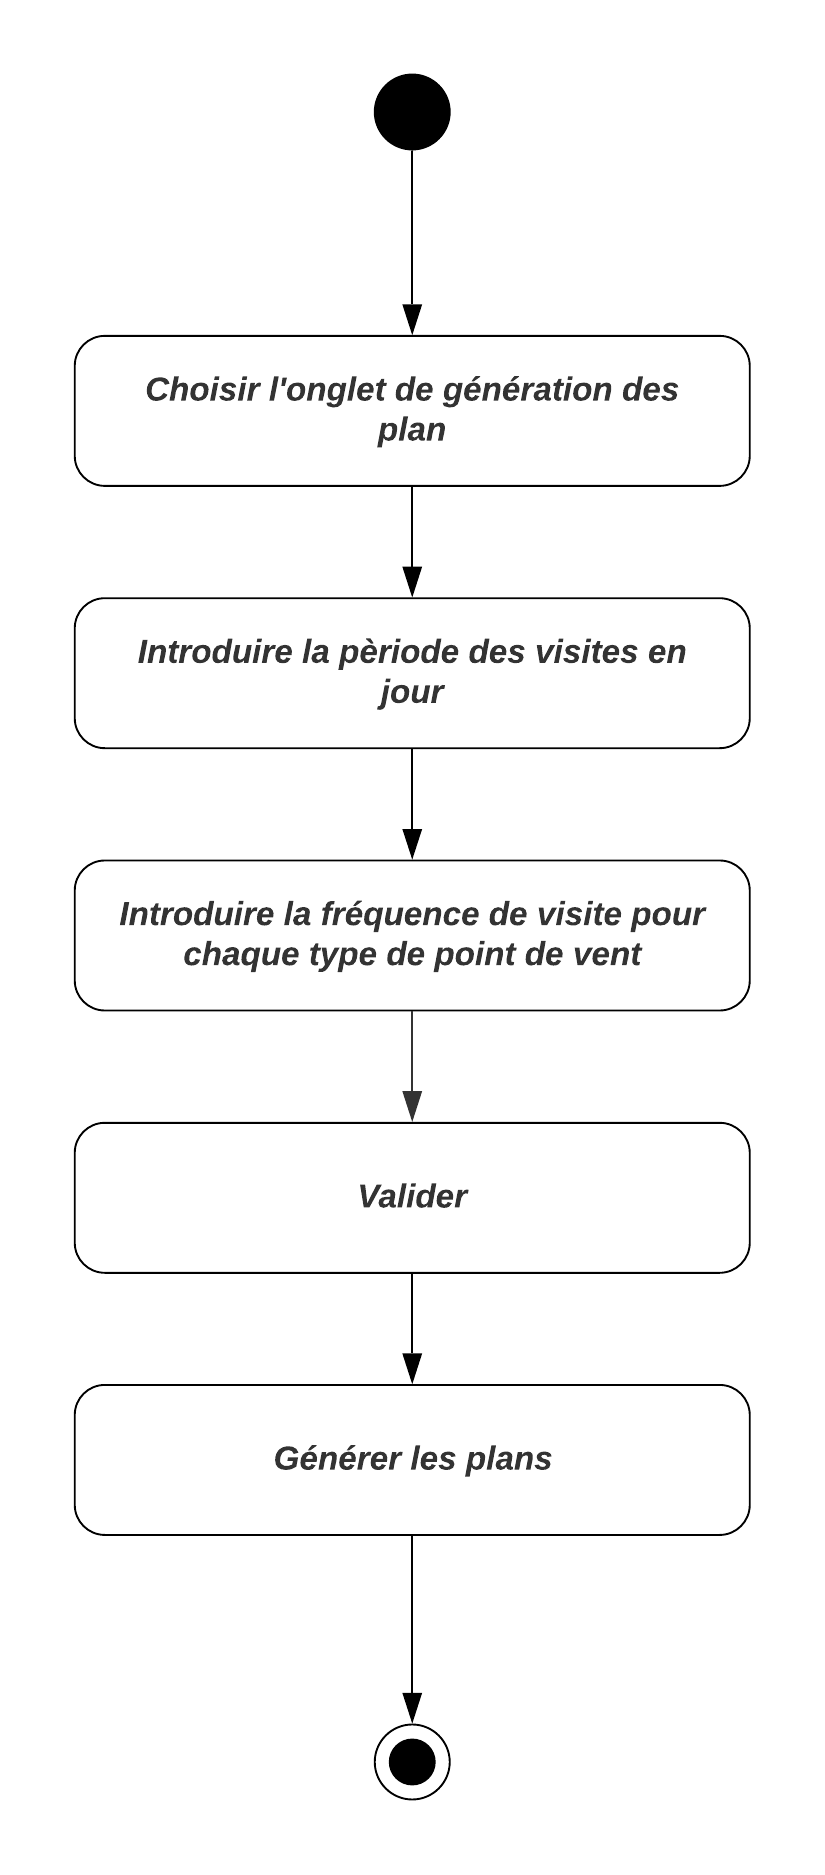
\includegraphics[height=17cm]{images_pfe/GENERATE_PLANS_DIAGRAM.png}
  \caption{Diagramme d'activité du CU: Générer les plans de visite des animateurs.}
  \label{fig:activity-admin}
\end{figure}
\FloatBarrier

\clearpage

\subsection{Animateur}


\begin{figure}[hbt!]
  \centering
  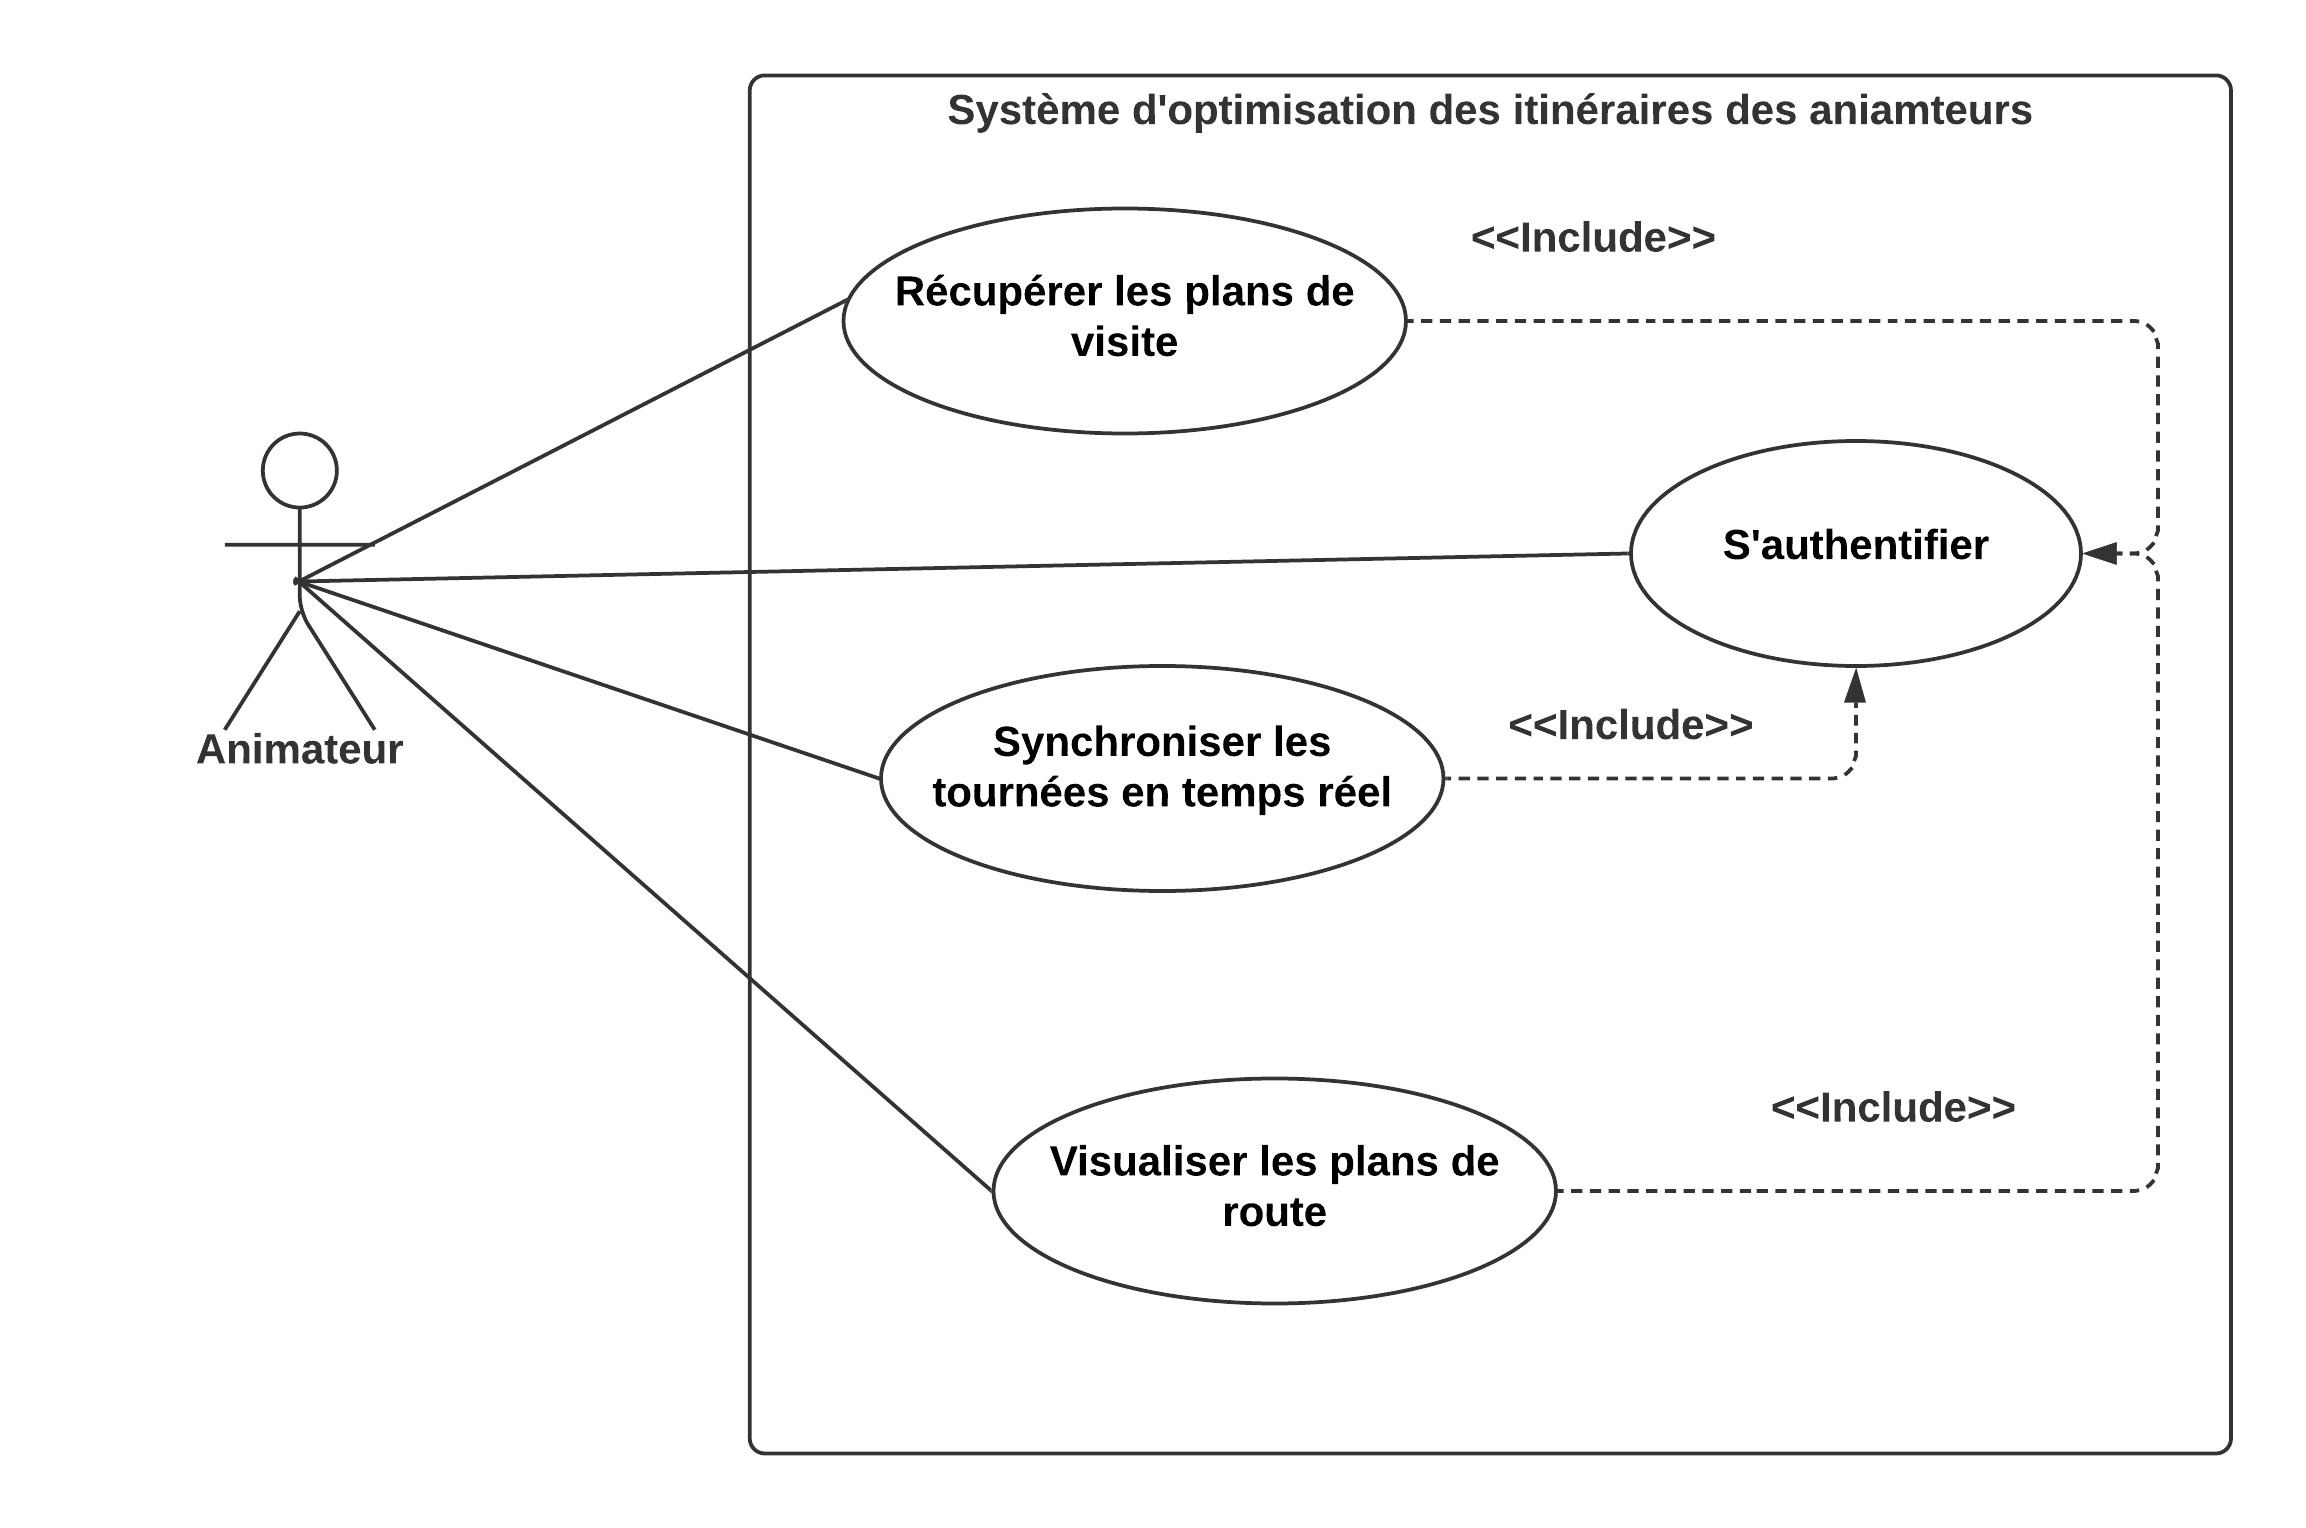
\includegraphics[width=\linewidth]{images_pfe/DCU_ANIMATEUR.png}
  \caption{Diagramme des cas d'utilisation de l'animateur.}
  \label{fig:dcu-animateur}
\end{figure}
\FloatBarrier

\renewcommand{\arraystretch}{1.5}
\begin{xltabular}{\linewidth}{|c|X|c|c|}
    \hline
    ID & CU & Documentation & Diagramme d'activité     \\\hline
    1 & S'authentifier & & \\ \hline
    10 & Récupérer les plans de visite & \checkmark & \\ \hline
    11 & Synchroniser les tournées & \checkmark & \checkmark \\ \hline
    12 & Visualiser les plans de route & & \\ \hline
    
    \caption{Liste des cas d'utilisation de l'animateur.}
    \label{tab:animator-use-cases}
\end{xltabular}
\FloatBarrier

\renewcommand{\arraystretch}{1.5}
\begin{xltabular}{\linewidth}{|X|}
    \hline
    \textbf{CU} : Récupérer les plans de visite    \\\hline
    \textbf{ID} :  10    \\\hline
    \textbf{Description brève} : Récupérer les plans de visite de l'animateur de pendant toute la période     \\\hline
    \textbf{Acteurs primaires} :   Animateur   \\\hline
    \textbf{Acteurs secondaires} : /     \\\hline
    \textbf{Pré condition} : L'animateur est déjà connecté   \\\hline
    \textbf{Enchaînement principal} : \\
    Le cas d'utilisation démarre lorsque l'animateur souhaite récupérer ses plans de visite.\\
    1. L'animateur choisit l'onglet plans de visite.\\
    2. Il lance la requête de récupération.\\
    3. Le système renvoie les plans de l'animateur.
    \\\hline
    \textbf{Post condition} :  Les plans de visite de l'animateur sont récupérés    \\\hline
    \textbf{Enchaînement alternatif} :  /   \\\hline
    
    \caption{Documentation CU : Récupérer les plans de visite.}
    \label{tab:cu-specs4}
\end{xltabular}
\FloatBarrier


\renewcommand{\arraystretch}{1.5}
\begin{xltabular}{\linewidth}{|X|}
    \hline
    \textbf{CU} : Synchroniser les tournées en temps réel     \\\hline
    \textbf{ID} :  11    \\\hline
    \textbf{Description brève} :  Mettre à jour la tournée par rapport à la fluidité du trafic routier    \\\hline
    \textbf{Acteurs primaires} :  Animateur    \\\hline
    \textbf{Acteurs secondaires} :   /   \\\hline
    \textbf{Pré condition} :   L'animateur est connecté   \\\hline
    \textbf{Enchaînement principal} :   \\
    Le cas d'utilisation démarre lorsque l'animateur souhaite synchroniser sa tournée.\\
    1. L'animateur choisit la section de synchronisation.\\
    2. L'animateur lance la requête de synchronisation.\\
    3. Le système renvoie la tournée synchronisée.
    \\\hline
    \textbf{Post condition} :  La tournée est synchronisée    \\\hline
    \textbf{Enchaînement alternatif} :  /    \\\hline
    
    \caption{Documentation CU : Synchroniser les tournées en temps réel.}
    \label{tab:cu-specs5}
\end{xltabular}
\FloatBarrier

\begin{figure}[hbt!]
  \centering
  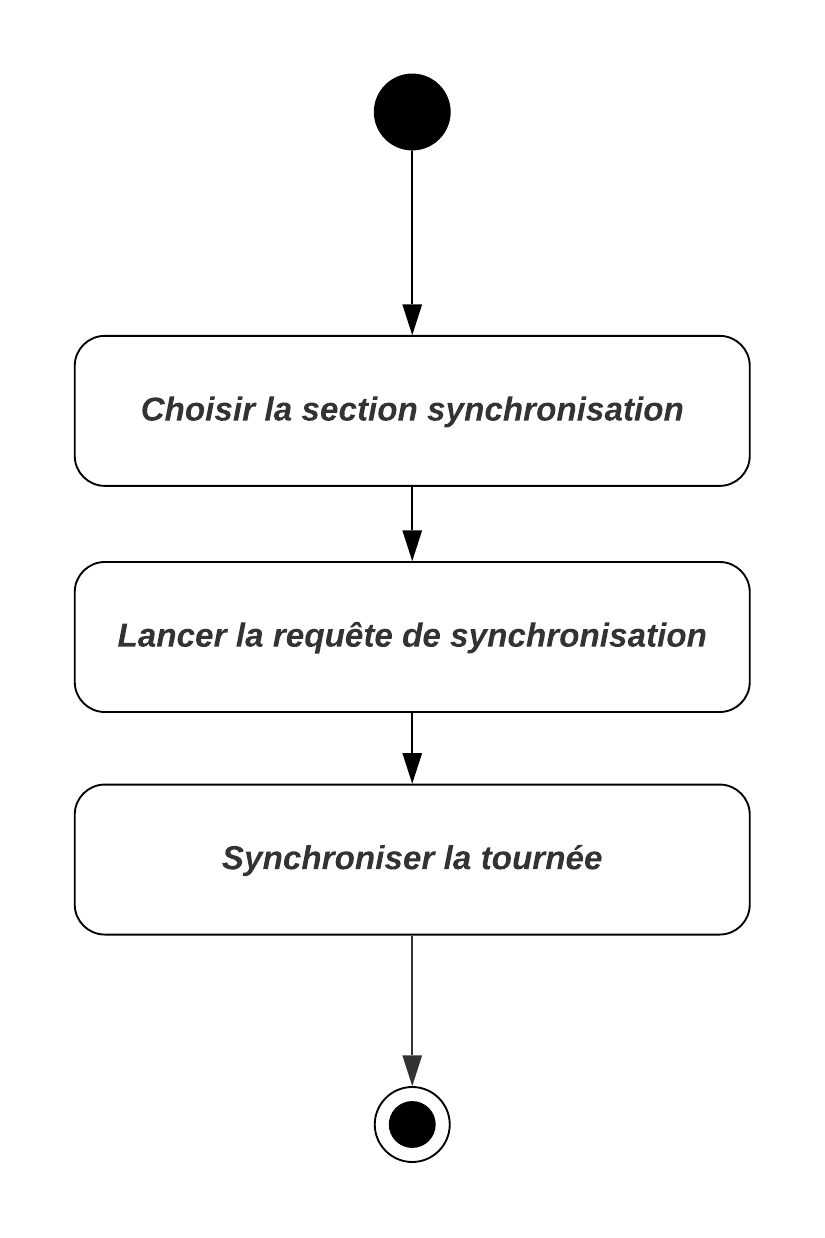
\includegraphics[height=13cm]{images_pfe/SYNC_TOUR_DIAGRAM.png}
  \caption{Diagramme d'activité du CU: Synchroniser les tournées en temps réel.}
  \label{fig:activity-animator}
\end{figure}
\FloatBarrier


\section{Conclusion}
Lorem ipsum dolor sit amet, consectetur adipiscing elit. Proin posuere euismod neque, non semper nibh viverra sed. Praesent ut varius magna. Fusce ipsum ante, semper nec interdum at, semper et lacus. Nulla ultrices magna a fringilla finibus. Etiam sollicitudin blandit ante. Vivamus blandit rhoncus tincidunt. Morbi sit amet congue purus. Praesent interdum gravida congue. Donec fermentum dui fermentum maximus rutrum.




%%% Local Variabs prles: 
%%% mode: latex
%%% TeX-master: "isae-report-template"
%%% End: 
\chapter{Conception}

\newpage

\section{Introduction}
Lorem ipsum dolor sit amet, consectetur adipiscing elit. Proin posuere euismod neque, non semper nibh viverra sed. Praesent ut varius magna. Fusce ipsum ante, semper nec interdum at, semper et lacus. Nulla ultrices magna a fringilla finibus. Etiam sollicitudin blandit ante. Vivamus blandit rhoncus tincidunt. Morbi sit amet congue purus. Praesent interdum gravida congue. Donec fermentum dui fermentum maximus rutrum.

\section{Rappel sur le besoin}
Lorem ipsum dolor sit amet, consectetur adipiscing elit. Proin posuere euismod neque, non semper nibh viverra sed. Praesent ut varius magna. Fusce ipsum ante, semper nec interdum at, semper et lacus. Nulla ultrices magna a fringilla finibus. Etiam sollicitudin blandit ante. Vivamus blandit rhoncus tincidunt. Morbi sit amet congue purus. Praesent interdum gravida congue. Donec fermentum dui fermentum maximus rutrum.

\medskip

Lorem ipsum dolor sit amet, consectetur adipiscing elit. Proin posuere euismod neque, non semper nibh viverra sed. Praesent ut varius magna. Fusce ipsum ante, semper nec interdum at, semper et lacus. Nulla ultrices magna a fringilla finibus. Etiam sollicitudin blandit ante. Vivamus blandit rhoncus tincidunt. Morbi sit amet congue purus. Praesent interdum gravida congue. Donec fermentum dui fermentum maximus rutrum. (Voir \ref{sec:pos}) Lorem ipsum dolor sit amet, consectetur adipiscing elit. Proin posuere euismod neque, non semper nibh viverra sed. Praesent ut varius magna. Fusce ipsum ante, semper nec interdum at, semper et lacus. Nulla ultrices magna a fringilla finibus. Etiam sollicitudin blandit ante. Vivamus blandit rhoncus tincidunt. Morbi sit amet congue purus. Praesent interdum gravida congue. Donec fermentum dui fermentum maximus rutrum.

\medskip

Lorem ipsum dolor sit amet, consectetur adipiscing elit. Proin posuere euismod neque, non semper nibh viverra sed. Praesent ut varius magna. Fusce ipsum ante, semper nec interdum at, semper et lacus. Nulla ultrices magna a fringilla finibus. Etiam sollicitudin blandit ante. Vivamus blandit rhoncus tincidunt. Morbi sit amet congue purus. Praesent interdum gravida congue. Donec fermentum dui fermentum maximus rutrum. :
\medskip

\begin{itemize}
    \item Les visites n'obéissent pas à une logique basée sur l'importance des points de vente.
    \item Les plans de routes ne sont pas optimaux en matière de temps et de distance.
\end{itemize}

\medskip

Lorem ipsum dolor sit amet, consectetur adipiscing elit. Proin posuere euismod neque, non semper nibh viverra sed. Praesent ut varius magna. Fusce ipsum ante, semper nec interdum at, semper et lacus. Nulla ultrices magna a fringilla finibus. Etiam sollicitudin blandit ante. Vivamus blandit rhoncus tincidunt. Morbi sit amet congue purus. Praesent interdum gravida congue. Donec fermentum dui fermentum maximus rutrum.

\begin{figure}[hbt!]
  \centering
  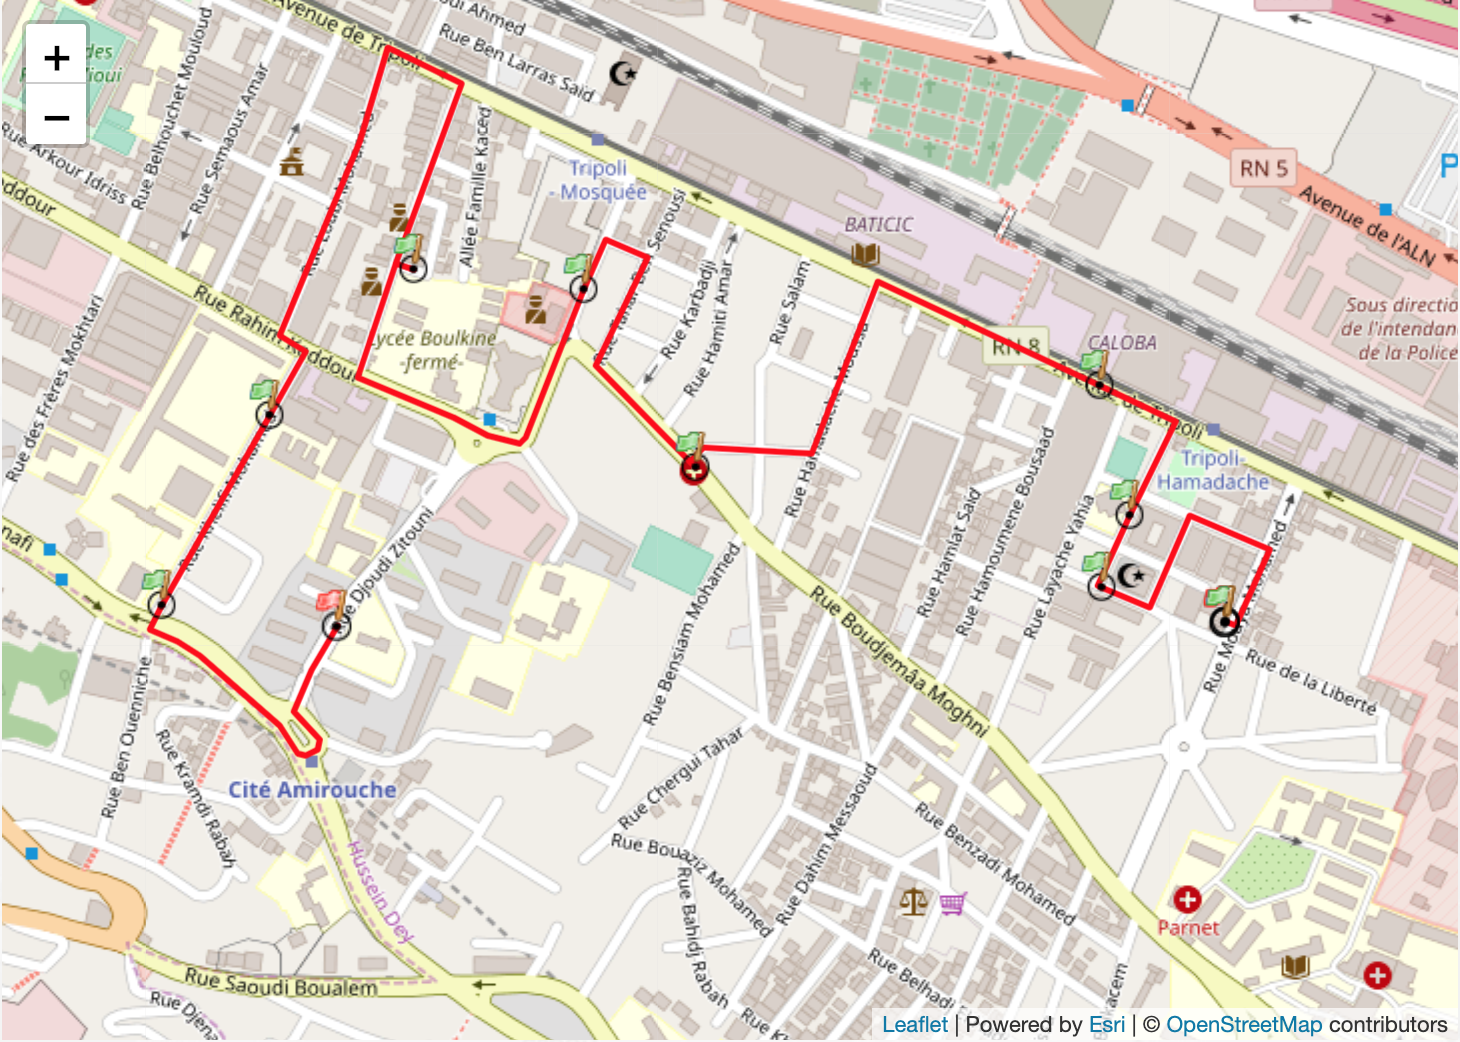
\includegraphics[height=8cm]{images_pfe/animator_route.png}
  \caption{Un exemple de tournée d'un animateur(en rouge).}
  \label{fig:tournee-animateur-example}
\end{figure}
\FloatBarrier

\section{Objectifs du système}
Lorem ipsum dolor sit amet, consectetur adipiscing elit. Proin posuere euismod neque, non semper nibh viverra sed. Praesent ut varius magna. Fusce ipsum ante, semper nec interdum at, semper et lacus. Nulla ultrices magna a fringilla finibus. Etiam sollicitudin blandit ante. Vivamus blandit rhoncus tincidunt. Morbi sit amet congue purus. Praesent interdum gravida congue. Donec fermentum dui fermentum maximus rutrum.Lorem ipsum dolor sit amet, consectetur adipiscing elit. Proin posuere euismod neque, non semper nibh viverra sed. Praesent ut varius magna. Fusce ipsum ante, semper nec interdum at, semper et lacus. Nulla ultrices magna a fringilla finibus. Etiam sollicitudin blandit ante. Vivamus blandit rhoncus tincidunt. Morbi sit amet congue purus. Praesent interdum gravida congue. Donec fermentum dui fermentum maximus rutrum.


\section{Présentation de la solution}
Lorem ipsum dolor sit amet, consectetur adipiscing elit. Proin posuere euismod neque, non semper nibh viverra sed. Praesent ut varius magna. Fusce ipsum ante, semper nec interdum at, semper et lacus. Nulla ultrices magna a fringilla finibus. Etiam sollicitudin blandit ante. Vivamus blandit rhoncus tincidunt. Morbi sit amet congue purus. Praesent interdum gravida congue. Donec fermentum dui fermentum maximus rutrum.

\medskip

Lorem ipsum dolor sit amet, consectetur adipiscing elit. Proin posuere euismod neque, non semper nibh viverra sed. Praesent ut varius magna. Fusce ipsum ante, semper nec interdum at, semper et lacus. Nulla ultrices magna a fringilla finibus. Etiam sollicitudin blandit ante. Vivamus blandit rhoncus tincidunt. Morbi sit amet congue purus. Praesent interdum gravida congue. Donec fermentum dui fermentum maximus rutrum.(Voir section \ref{sec:hotspot}). Lorem ipsum dolor sit amet, consectetur adipiscing elit. Proin posuere euismod neque, non semper nibh viverra sed. Praesent ut varius magna. Fusce ipsum ante, semper nec interdum at, semper et lacus. Nulla ultrices magna a fringilla finibus. Etiam sollicitudin blandit ante. Vivamus blandit rhoncus tincidunt. Morbi sit amet congue purus. Praesent interdum gravida congue. Donec fermentum dui fermentum maximus rutrum.
\medskip
Lorem ipsum dolor sit amet, consectetur adipiscing elit. Proin posuere euismod neque, non semper nibh viverra sed. Praesent ut varius magna. Fusce ipsum ante, semper nec interdum at, semper et lacus. Nulla ultrices magna a fringilla finibus. Etiam sollicitudin blandit ante. Vivamus blandit rhoncus tincidunt. Morbi sit amet congue purus. Praesent interdum gravida congue. Donec fermentum dui fermentum maximus rutrum.(Voir section \ref{sec:ptsp}). Lorem ipsum dolor sit amet, consectetur adipiscing elit. Proin posuere euismod neque, non semper nibh viverra sed. Praesent ut varius magna. Fusce ipsum ante, semper nec interdum at, semper et lacus. Nulla ultrices magna a fringilla finibus. Etiam sollicitudin blandit ante. Vivamus blandit rhoncus tincidunt. Morbi sit amet congue purus. Praesent interdum gravida congue. Donec fermentum dui fermentum maximus rutrum.

\medskip

Lorem ipsum dolor sit amet, consectetur adipiscing elit. Proin posuere euismod neque, non semper nibh viverra sed. Praesent ut varius magna. Fusce ipsum ante, semper nec interdum at, semper et lacus. Nulla ultrices magna a fringilla finibus. Etiam sollicitudin blandit ante. Vivamus blandit rhoncus tincidunt. Morbi sit amet congue purus. Praesent interdum gravida congue. Donec fermentum dui fermentum maximus rutrum.

\medskip

Lorem ipsum dolor sit amet, consectetur adipiscing elit. Proin posuere euismod neque, non semper nibh viverra sed. Praesent ut varius magna. Fusce ipsum ante, semper nec interdum at, semper et lacus. Nulla ultrices magna a fringilla finibus. Etiam sollicitudin blandit ante. Vivamus blandit rhoncus tincidunt. Morbi sit amet congue purus. Praesent interdum gravida congue. Donec fermentum dui fermentum maximus rutrum. :

\medskip

\begin{figure}[hbt!]
  \centering
  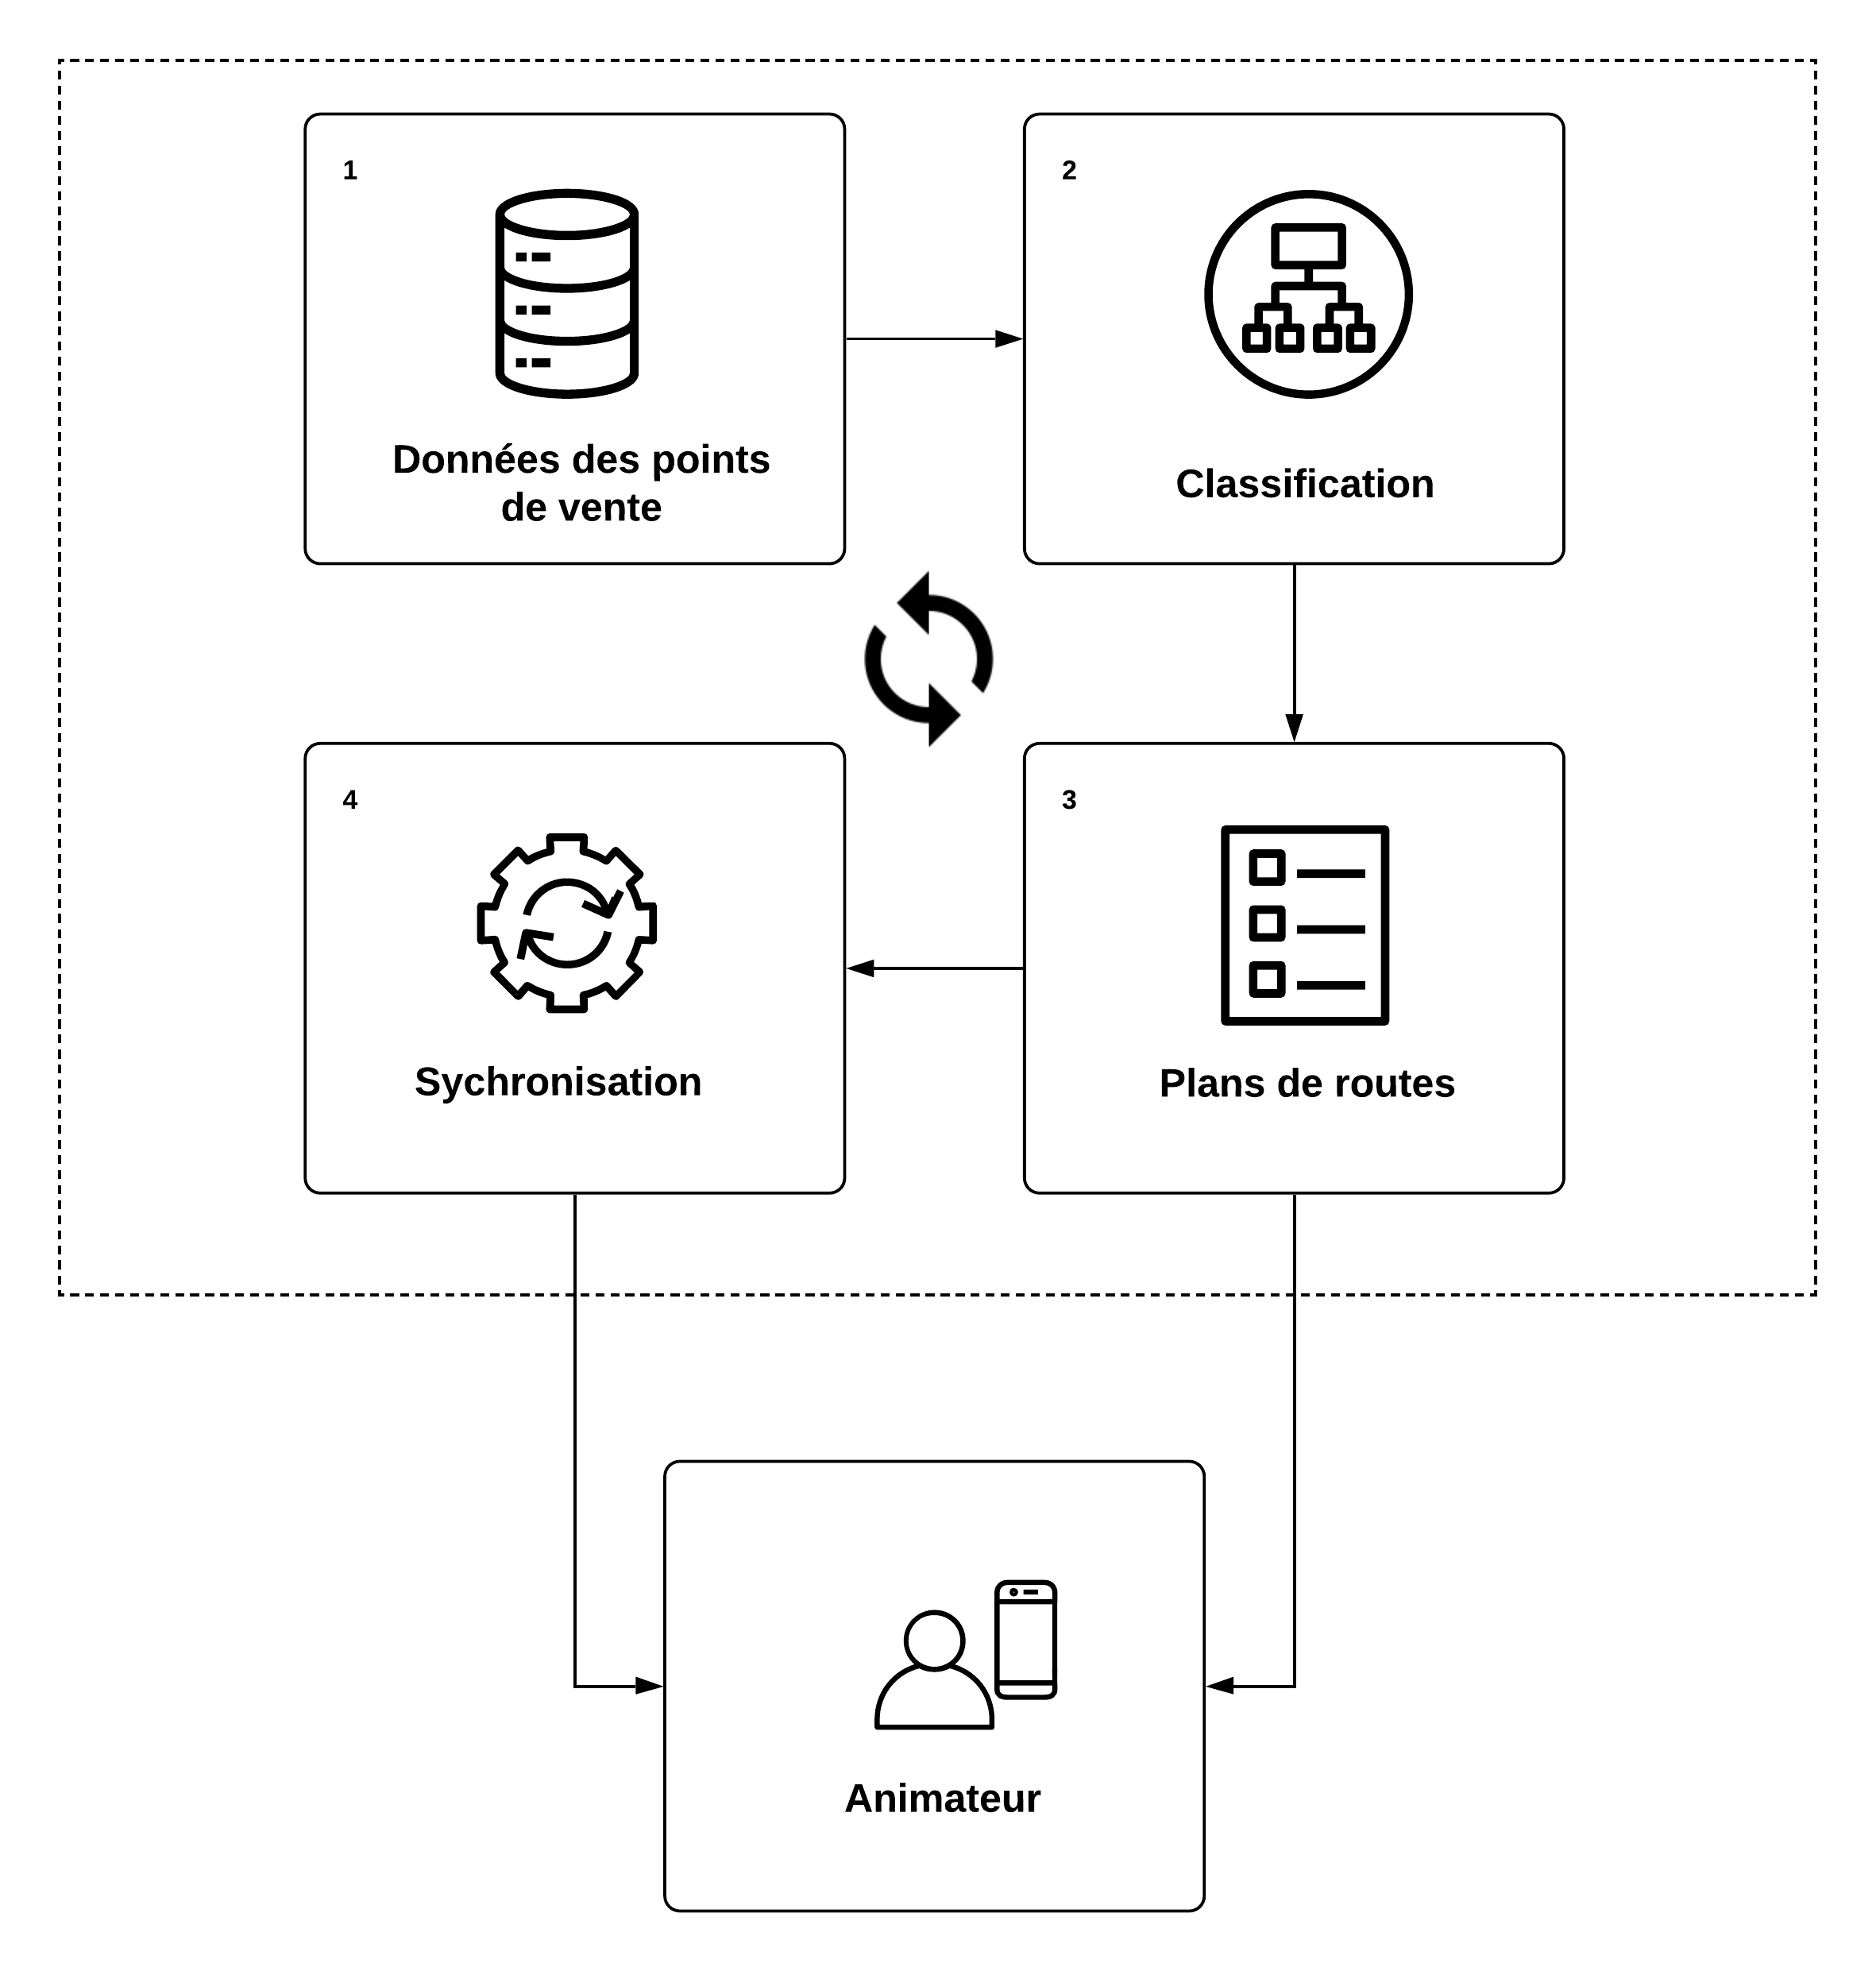
\includegraphics[width=8cm]{images_pfe/Optimization_Process.png}
  \caption{Processus d'élaboration des plans de route.}
  \label{fig:optimisation-process}
\end{figure}
\FloatBarrier

Lorem ipsum dolor sit amet, consectetur adipiscing elit. Proin posuere euismod neque, non semper nibh viverra sed. Praesent ut varius magna. Fusce ipsum ante, semper nec interdum at, semper et lacus. Nulla ultrices magna a fringilla finibus. Etiam sollicitudin blandit ante. Vivamus blandit rhoncus tincidunt. Morbi sit amet congue purus. Praesent interdum gravida congue. Donec fermentum dui fermentum maximus rutrum.



\section{Architecture fonctionnelle de la solution}

\begin{figure}[hbt!]
  \centering
  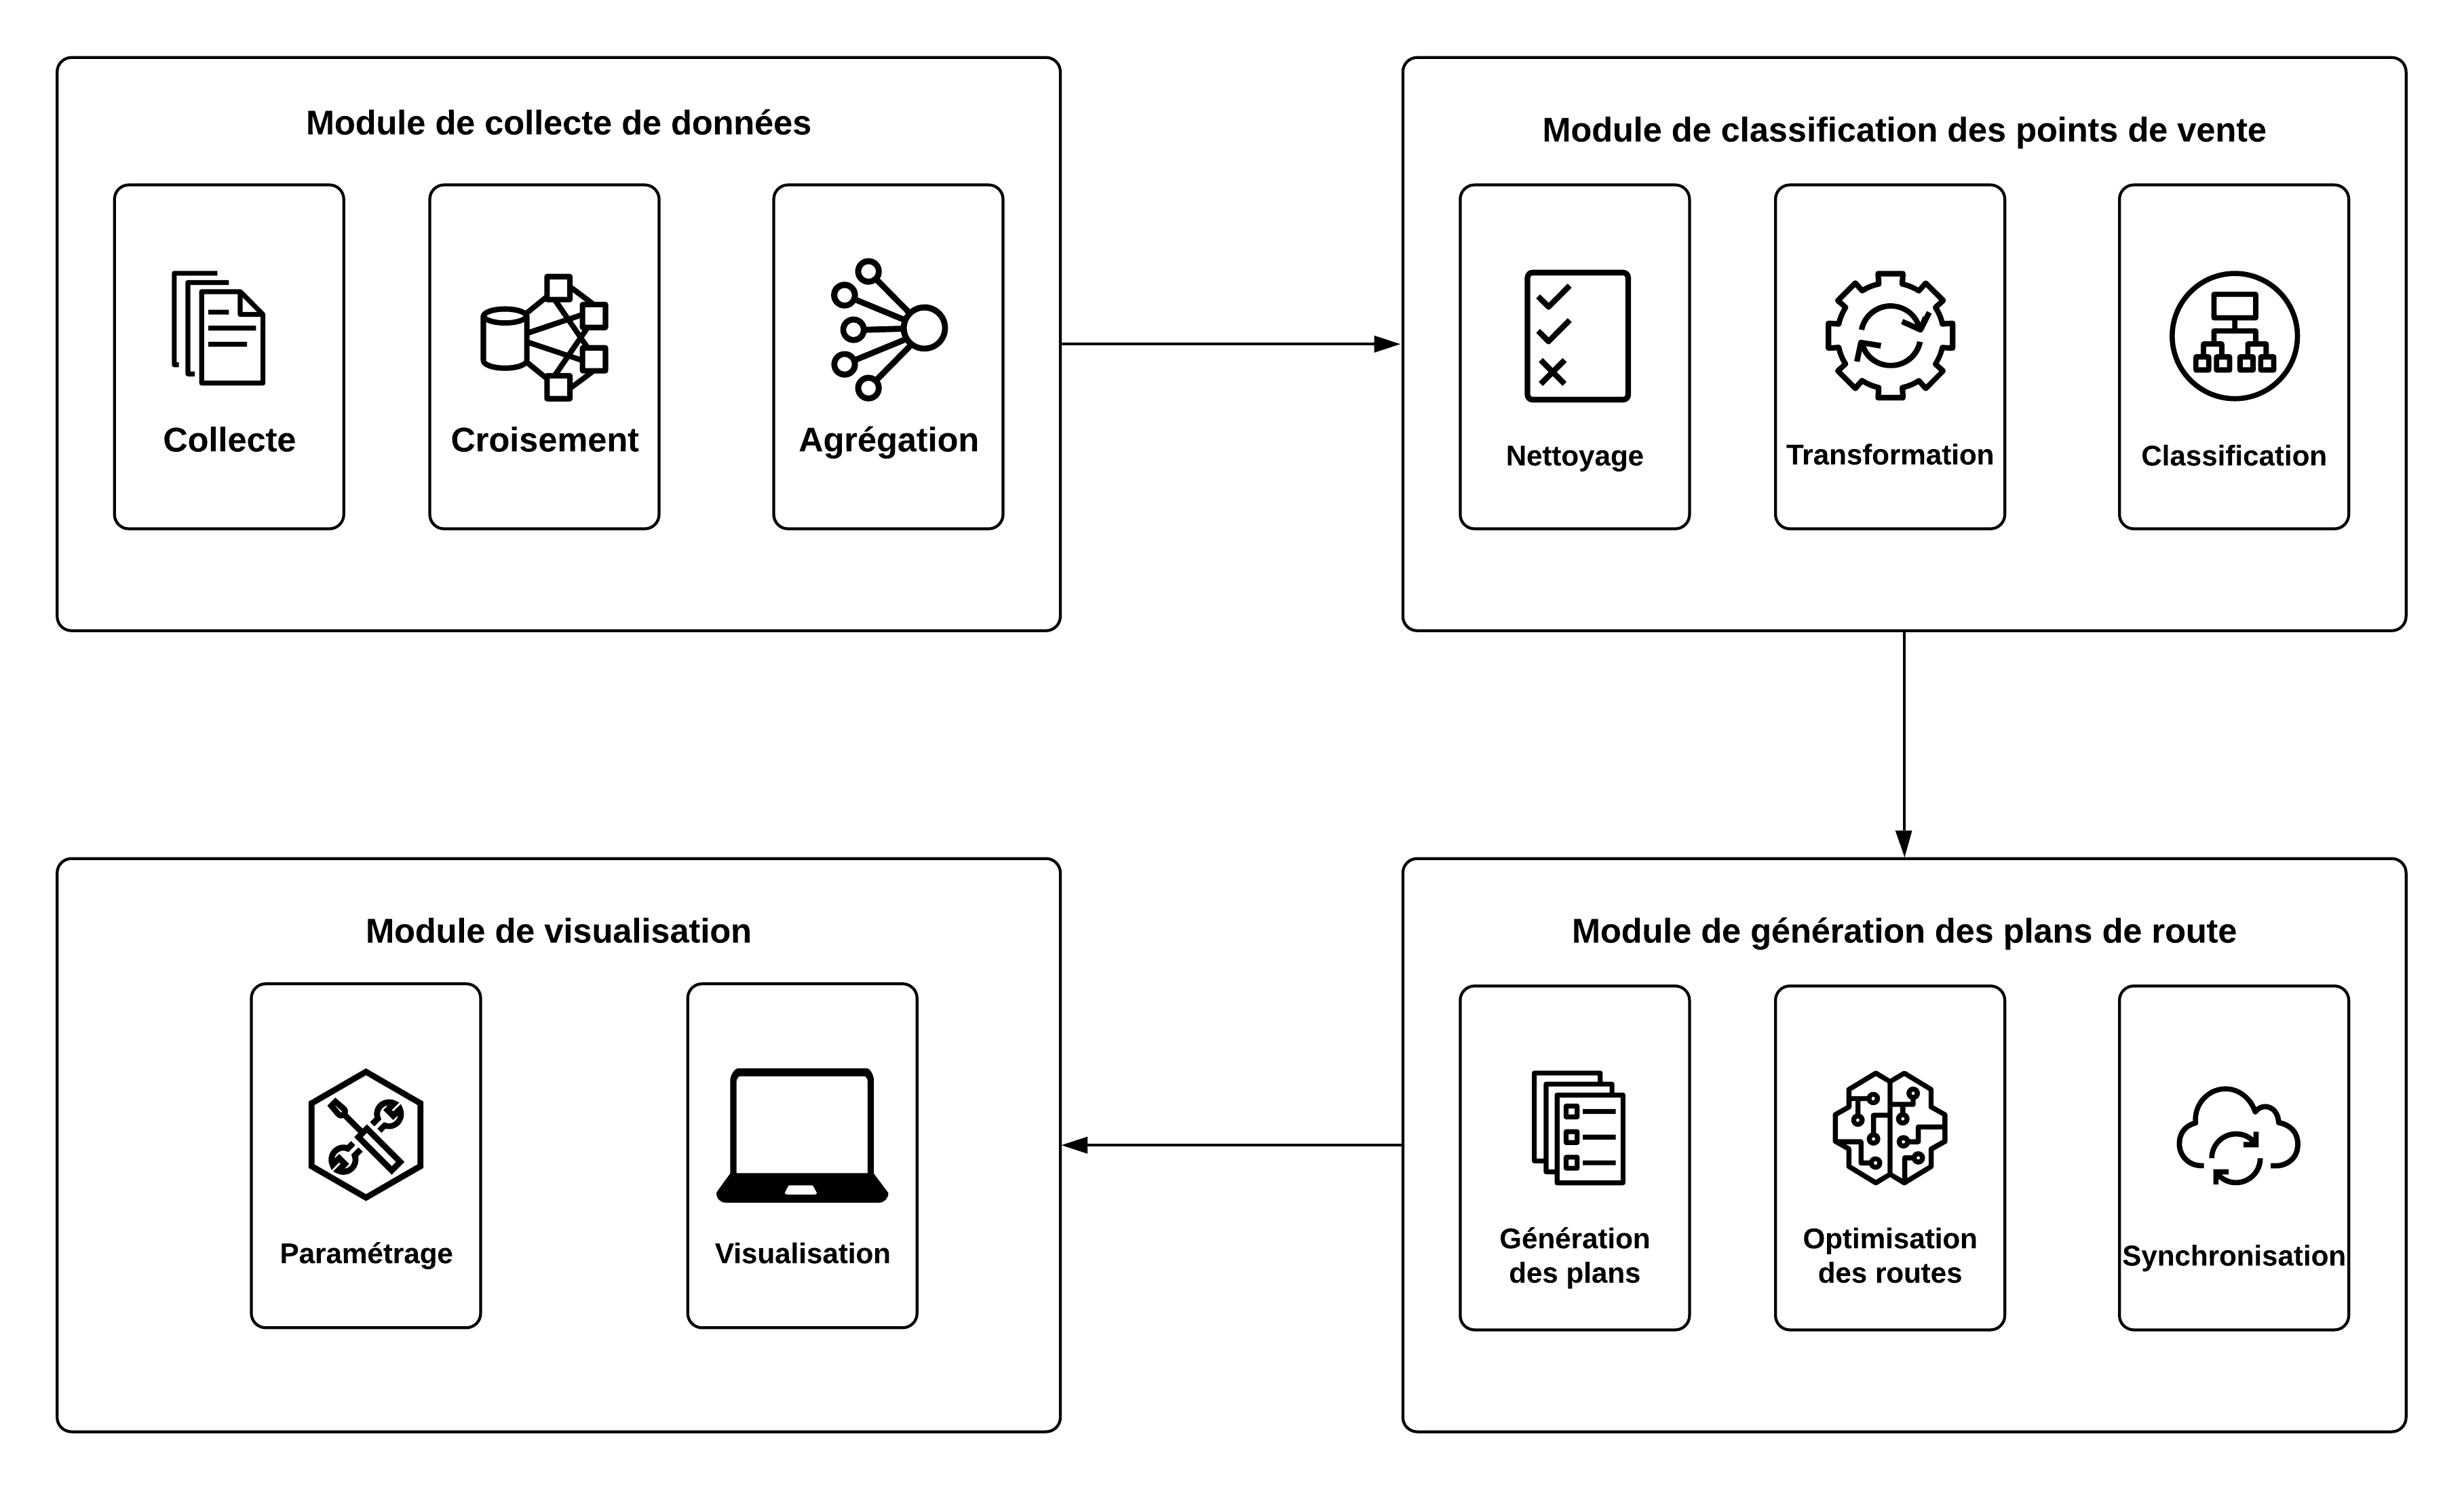
\includegraphics[height=10cm]{images_pfe/SYSTEM_COMPONENTS.png}
  \caption{Architecture fonctionnelle du système.}
  \label{fig:functional-architecture}
\end{figure}
\FloatBarrier 


Pour implémenter la solution proposée, certains modules sont nécessaires:
\begin{enumerate}
    \item \textbf{Module de collecte de données} : Lorem ipsum dolor sit amet, consectetur adipiscing elit. Proin posuere euismod neque, non semper nibh viverra sed. Praesent ut varius magna. Fusce ipsum ante, semper nec interdum at, semper et lacus. Nulla ultrices magna a fringilla finibus. Etiam sollicitudin blandit ante. Vivamus blandit rhoncus tincidunt. Morbi sit amet congue purus. Praesent interdum gravida congue. Donec fermentum dui fermentum maximus rutrum. 
    \item \textbf{Module de classification des points de vente} : Lorem ipsum dolor sit amet, consectetur adipiscing elit. Proin posuere euismod neque, non semper nibh viverra sed. Praesent ut varius magna. Fusce ipsum ante, semper nec interdum at, semper et lacus. Nulla ultrices magna a fringilla finibus. Etiam sollicitudin blandit ante. Vivamus blandit rhoncus tincidunt. Morbi sit amet congue purus. Praesent interdum gravida congue. Donec fermentum dui fermentum maximus rutrum.
    \item \textbf{Module de générations des plans de route} : Lorem ipsum dolor sit amet, consectetur adipiscing elit. Proin posuere euismod neque, non semper nibh viverra sed. Praesent ut varius magna. Fusce ipsum ante, semper nec interdum at, semper et lacus. Nulla ultrices magna a fringilla finibus. Etiam sollicitudin blandit ante. Vivamus blandit rhoncus tincidunt. Morbi sit amet congue purus. Praesent interdum gravida congue. Donec fermentum dui fermentum maximus rutrum.
    \item \textbf{Module de visualisation}: Lorem ipsum dolor sit amet, consectetur adipiscing elit. Proin posuere euismod neque, non semper nibh viverra sed. Praesent ut varius magna. Fusce ipsum ante, semper nec interdum at, semper et lacus. Nulla ultrices magna a fringilla finibus. Etiam sollicitudin blandit ante. Vivamus blandit rhoncus tincidunt. Morbi sit amet congue purus. Praesent interdum gravida congue. Donec fermentum dui fermentum maximus rutrum.
\end{enumerate}






\section{Les étapes de la solution}
Lorem ipsum dolor sit amet, consectetur adipiscing elit. Proin posuere euismod neque, non semper nibh viverra sed. Praesent ut varius magna. Fusce ipsum ante, semper nec interdum at, semper et lacus. Nulla ultrices magna a fringilla finibus. Etiam sollicitudin blandit ante. Vivamus blandit rhoncus tincidunt. Morbi sit amet congue purus. Praesent interdum gravida congue. Donec fermentum dui fermentum maximus rutrum. (Voir la figure \ref{fig:etapes-solution}). Dans ce qui suit nous détaillons chaque étape.


\begin{figure}[hbt!]
  \centering
  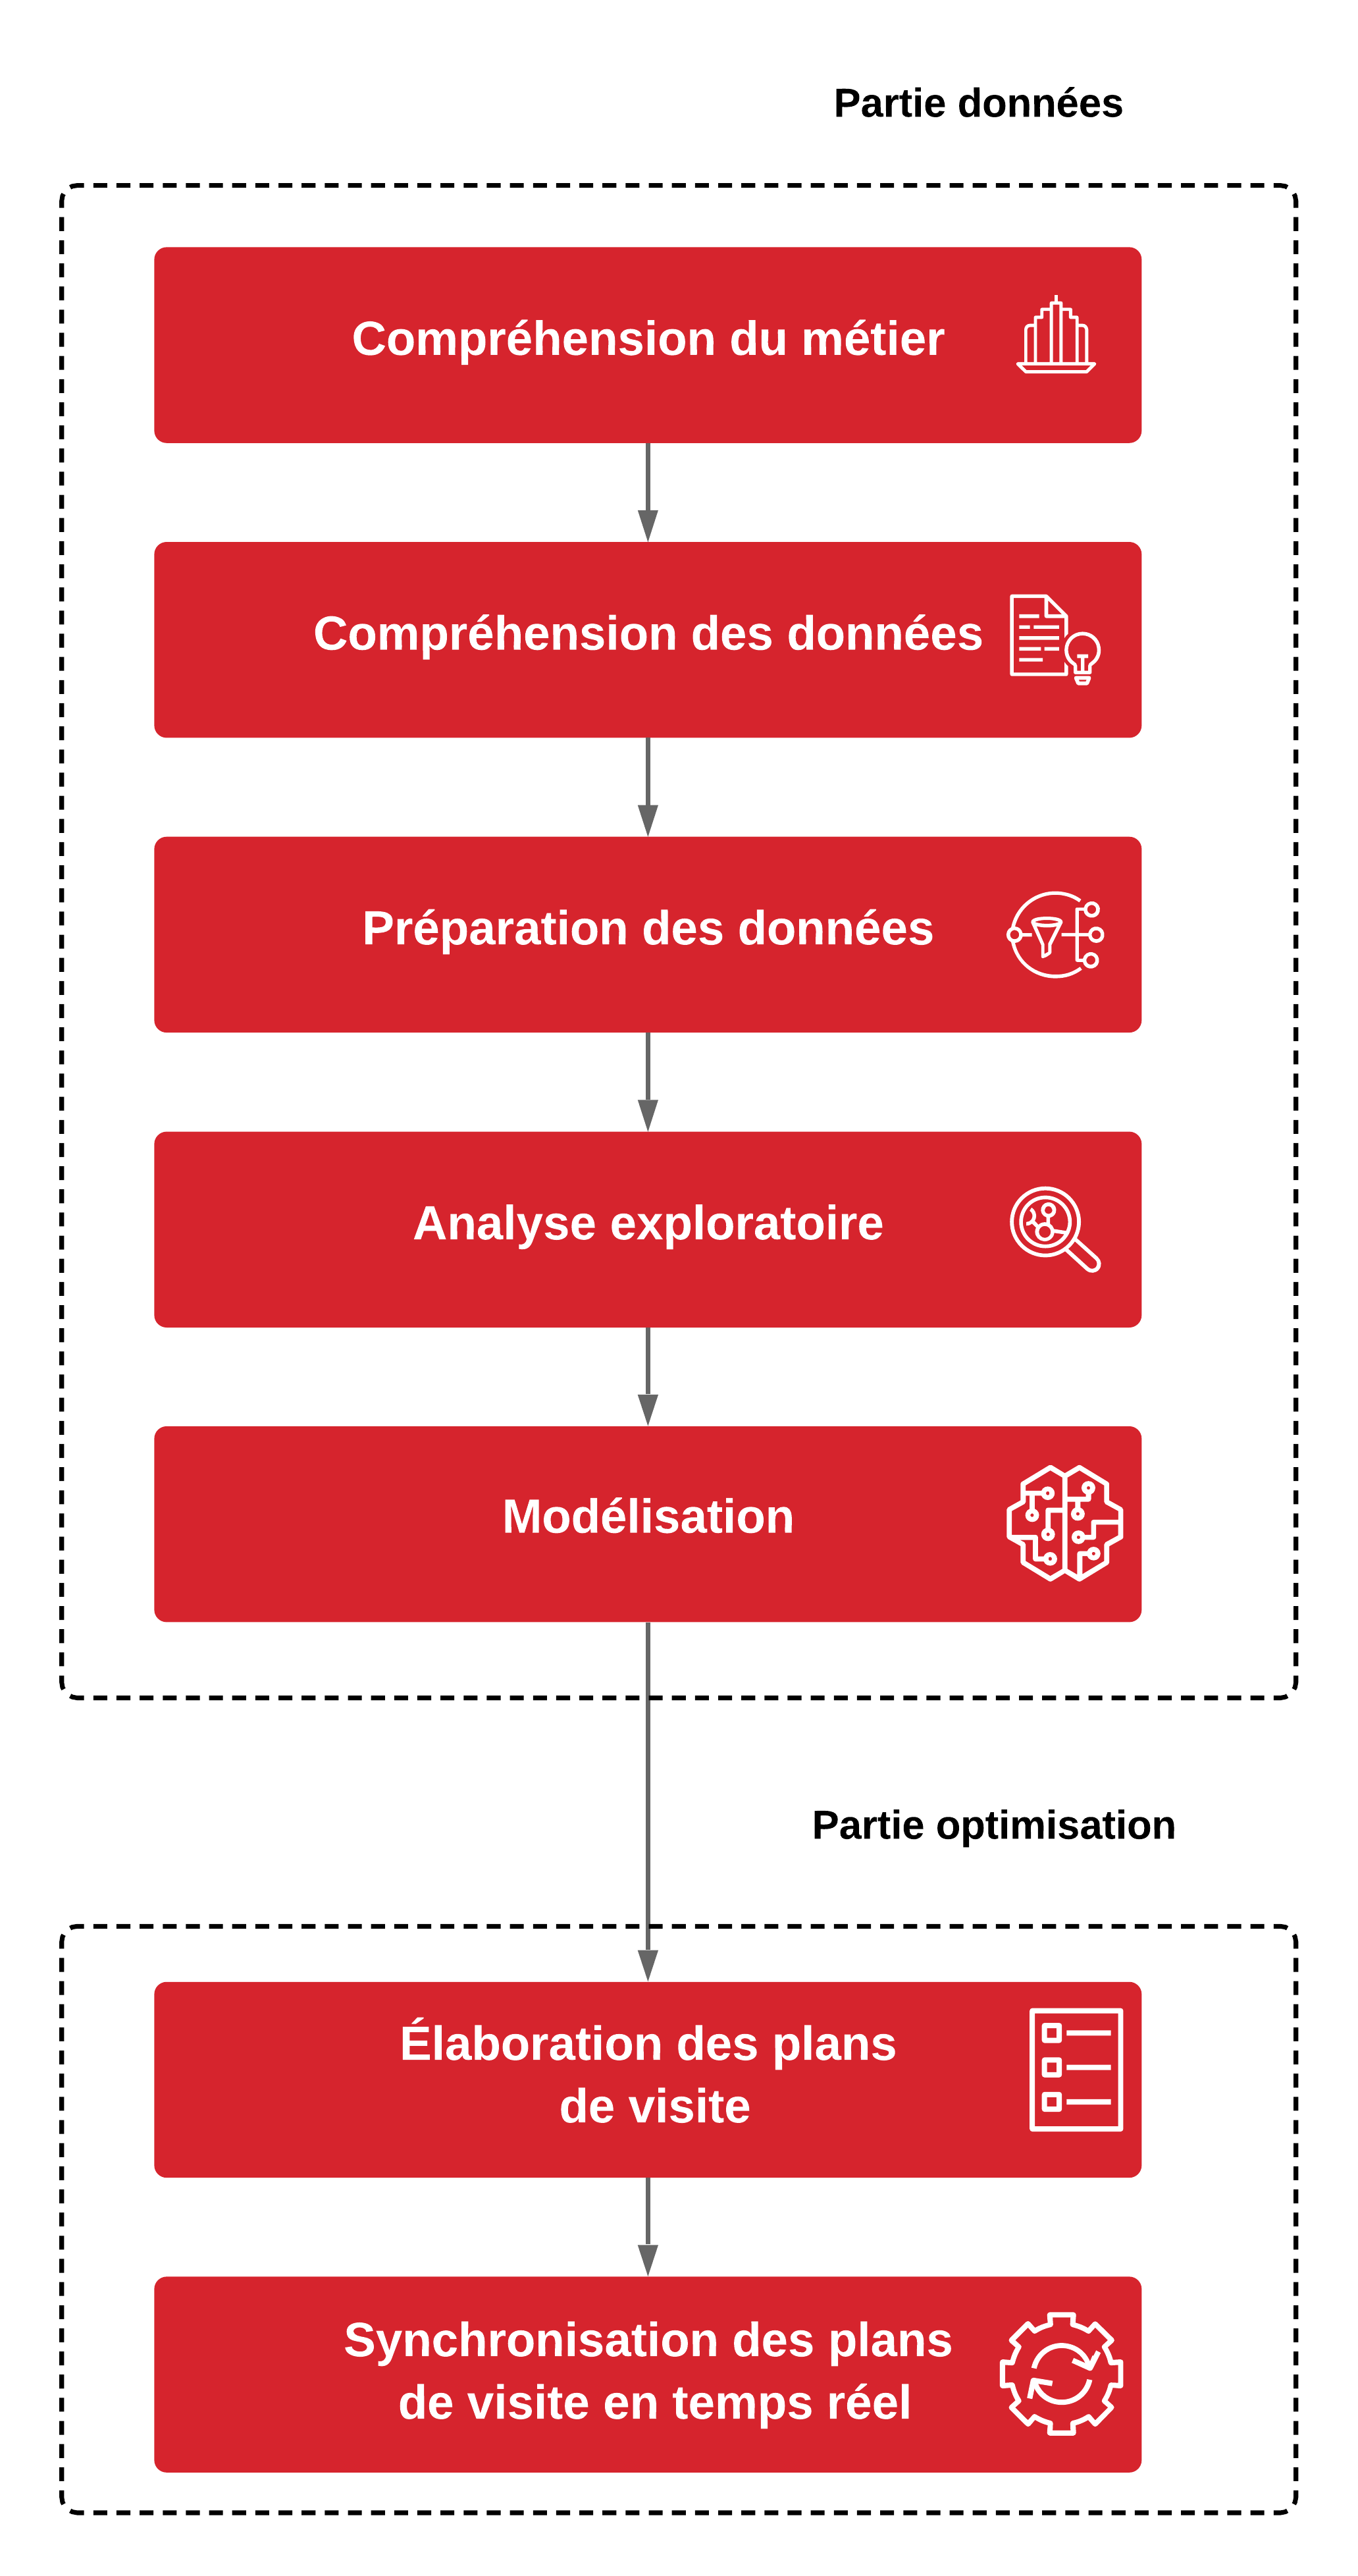
\includegraphics[height=12cm]{images_pfe/Etapes_solution.png}
  \caption{Les étapes de la solution.}
  \label{fig:etapes-solution}
\end{figure}
\FloatBarrier

\subsection{Compréhension du métier}
Lorem ipsum dolor sit amet, consectetur adipiscing elit. Proin posuere euismod neque, non semper nibh viverra sed. Praesent ut varius magna. Fusce ipsum ante, semper nec interdum at, semper et lacus. Nulla ultrices magna a fringilla finibus. Etiam sollicitudin blandit ante. Vivamus blandit rhoncus tincidunt. Morbi sit amet congue purus. Praesent interdum gravida congue. Donec fermentum dui fermentum maximus rutrum.Lorem ipsum dolor sit amet, consectetur adipiscing elit. Proin posuere euismod neque, non semper nibh viverra sed. Praesent ut varius magna. Fusce ipsum ante, semper nec interdum at, semper et lacus. Nulla ultrices magna a fringilla finibus. Etiam sollicitudin blandit ante. Vivamus blandit rhoncus tincidunt. Morbi sit amet congue purus. Praesent interdum gravida congue. Donec fermentum dui fermentum maximus rutrum.

\subsection{Compréhension des données}
Lorem ipsum dolor sit amet, consectetur adipiscing elit. Proin posuere euismod neque, non semper nibh viverra sed. Praesent ut varius magna. Fusce ipsum ante, semper nec interdum at, semper et lacus. Nulla ultrices magna a fringilla finibus. Etiam sollicitudin blandit ante. Vivamus blandit rhoncus tincidunt. Morbi sit amet congue purus. Praesent interdum gravida congue. Donec fermentum dui fermentum maximus rutrum.

\subsection{Préparation des données}
Lorem ipsum dolor sit amet, consectetur adipiscing elit. Proin posuere euismod neque, non semper nibh viverra sed. Praesent ut varius magna. Fusce ipsum ante, semper nec interdum at, semper et lacus. Nulla ultrices magna a fringilla finibus. Etiam sollicitudin blandit ante. Vivamus blandit rhoncus tincidunt. Morbi sit amet congue purus. Praesent interdum gravida congue. Donec fermentum dui fermentum maximus rutrum. (Voir la figure \ref{fig:dataset-columns}). Lorem ipsum dolor sit amet, consectetur adipiscing elit. Proin posuere euismod neque, non semper nibh viverra sed. Praesent ut varius magna. Fusce ipsum ante, semper nec interdum at, semper et lacus. Nulla ultrices magna a fringilla finibus. Etiam sollicitudin blandit ante. Vivamus blandit rhoncus tincidunt. Morbi sit amet congue purus. Praesent interdum gravida congue. Donec fermentum dui fermentum maximus rutrum.

\begin{figure}[hbt!]
  \centering
  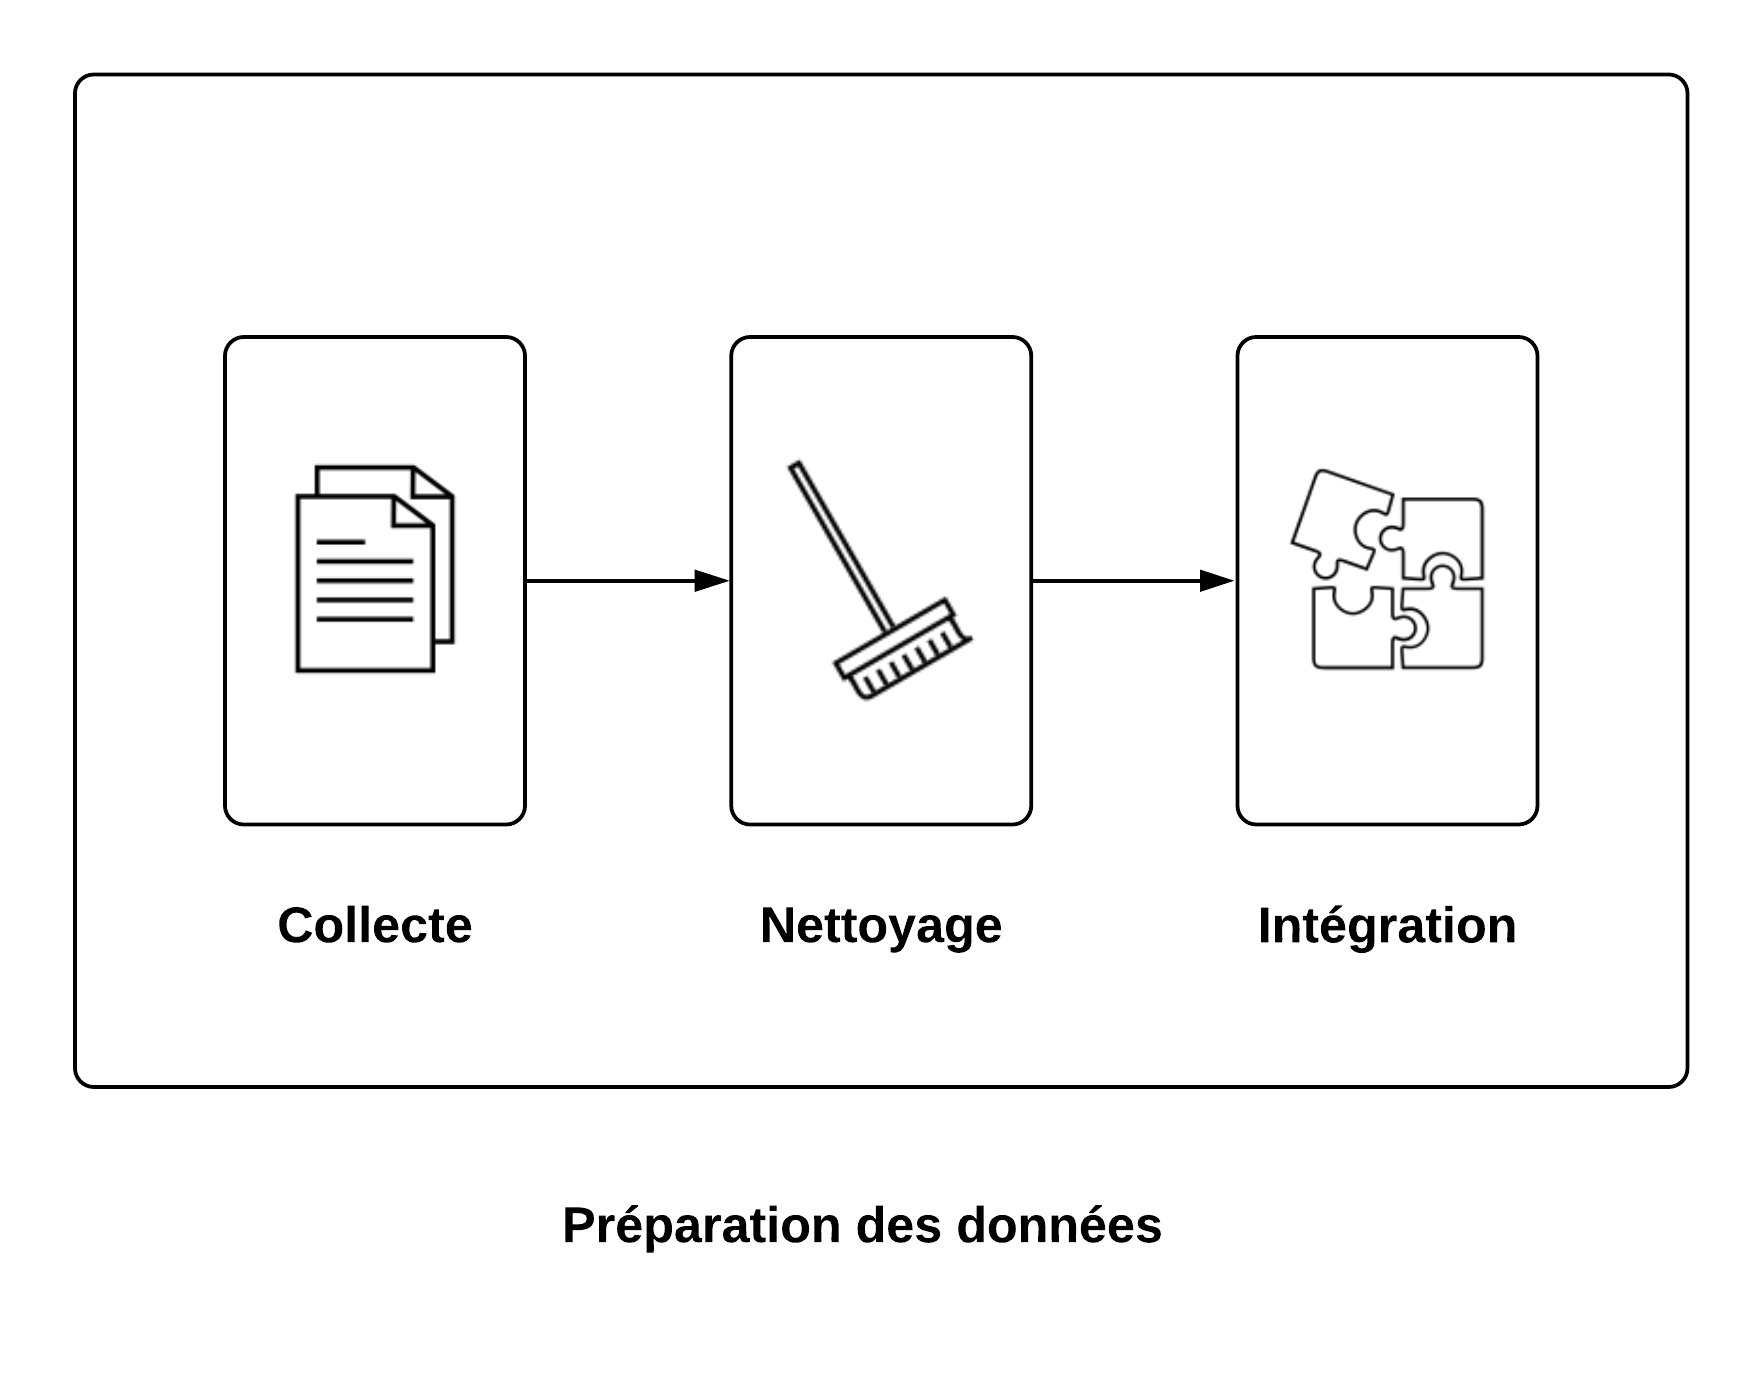
\includegraphics[width=10cm]{images_pfe/DATA_PREPARATION.png}
  \caption{Les étapes de préparation des données}
  \label{fig:data-preparation}
\end{figure}
\FloatBarrier

\begin{figure}[hbt!]
  \centering
  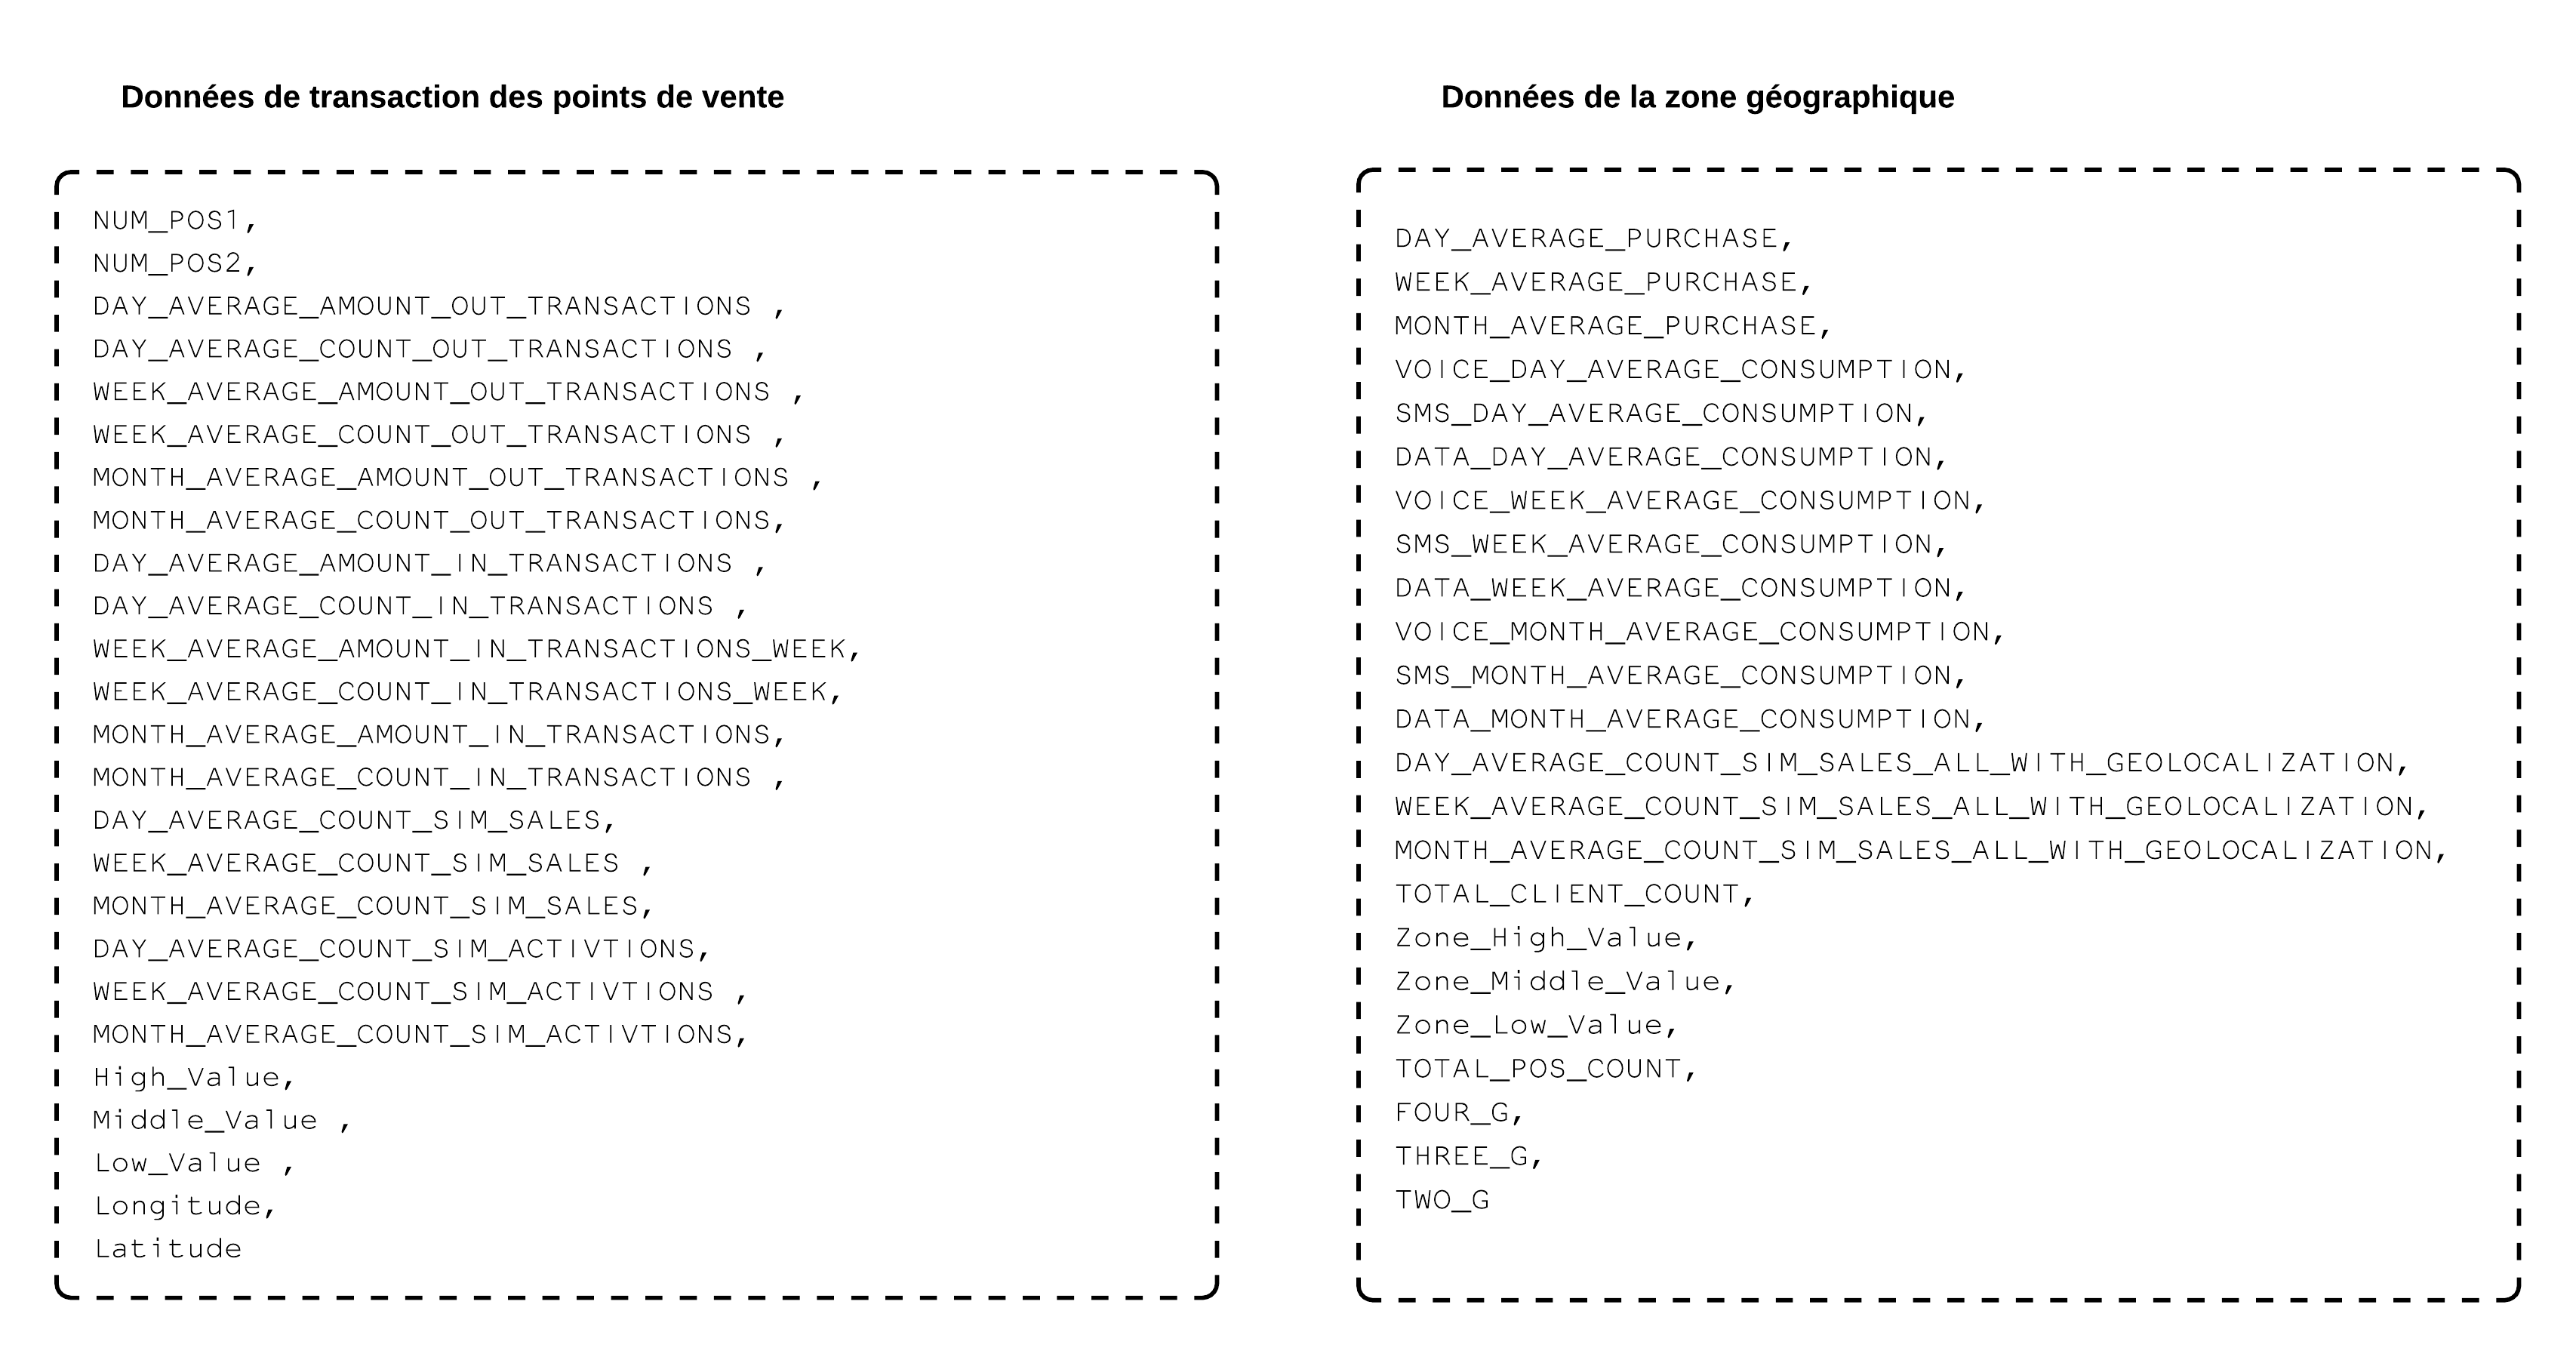
\includegraphics[width=16cm]{images_pfe/DATASET_COLUMNS.png}
  \caption{L'ensemble des attributs constituants le dataset initial (Voir les détails en annexe \ref{app:initial-dataset}).}
  \label{fig:dataset-columns}
\end{figure}
\FloatBarrier




\textbf{Quelques remarques} :
\renewcommand{\labelitemi}{$\bullet$}
\begin{itemize}
    \item Lorem ipsum dolor sit amet, consectetur adipiscing elit. Proin posuere euismod neque, non semper nibh viverra sed. Praesent ut varius magna. Fusce ipsum ante, semper nec interdum at, semper et lacus.
    \item Lorem ipsum dolor sit amet, consectetur adipiscing elit. Proin posuere euismod neque, non semper nibh viverra sed. Praesent ut varius magna. Fusce ipsum ante, semper nec interdum at, semper et lacus.
    \item Lorem ipsum dolor sit amet, consectetur adipiscing elit. Proin posuere euismod neque, non semper nibh viverra sed. Praesent ut varius magna. Fusce ipsum ante, semper nec interdum at, semper et lacus.
    \item Lorem ipsum dolor sit amet, consectetur adipiscing elit. Proin posuere euismod neque, non semper nibh viverra sed. Praesent ut varius magna. Fusce ipsum ante, semper nec interdum at, semper et lacus.
    \item Lorem ipsum dolor sit amet, consectetur adipiscing elit. Proin posuere euismod neque, non semper nibh viverra sed. Praesent ut varius magna. Fusce ipsum ante, semper nec interdum at, semper et lacus. BTS \footnote{Base Transceiver Station: antenne émettrice-réceptrice de signaux radioélectriques pour les communications mobiles qui convertit des signaux électriques en ondes électromagnétiques (et réciproquement)} Lorem ipsum dolor sit amet, consectetur adipiscing elit. Proin posuere euismod neque, non semper nibh viverra sed. Praesent ut varius magna. Fusce ipsum ante, semper nec interdum at, semper et lacus.
    
\end{itemize}



\subsection{Analyse exploratoire}
Lorem ipsum dolor sit amet, consectetur adipiscing elit. Proin posuere euismod neque, non semper nibh viverra sed. Praesent ut varius magna. Fusce ipsum ante, semper nec interdum at, semper et lacus. Nulla ultrices magna a fringilla finibus. Etiam sollicitudin blandit ante. Vivamus blandit rhoncus tincidunt. Morbi sit amet congue purus. Praesent interdum gravida congue. Donec fermentum dui fermentum maximus rutrum. Nous réaliserons ensuite, une analyse des Hotspots (Voir section \ref{sec:hotspot}) Lorem ipsum dolor sit amet, consectetur adipiscing elit. Proin posuere euismod neque, non semper nibh viverra sed. Praesent ut varius magna. Fusce ipsum ante, semper nec interdum at, semper et lacus. Nulla ultrices magna a fringilla finibus. Etiam sollicitudin blandit ante. Vivamus blandit rhoncus tincidunt. Morbi sit amet congue purus. Praesent interdum gravida congue. Donec fermentum dui fermentum maximus rutrum. (Voir \ref{subsec-gi-star}). Lorem ipsum dolor sit amet, consectetur adipiscing elit. Proin posuere euismod neque, non semper nibh viverra sed. Praesent ut varius magna. Fusce ipsum ante, semper nec interdum at, semper et lacus. Nulla ultrices magna a fringilla finibus. Etiam sollicitudin blandit ante. Vivamus blandit rhoncus tincidunt. Morbi sit amet congue purus. Praesent interdum gravida congue. Donec fermentum dui fermentum maximus rutrum.

\begin{figure}[hbt!]
  \centering
  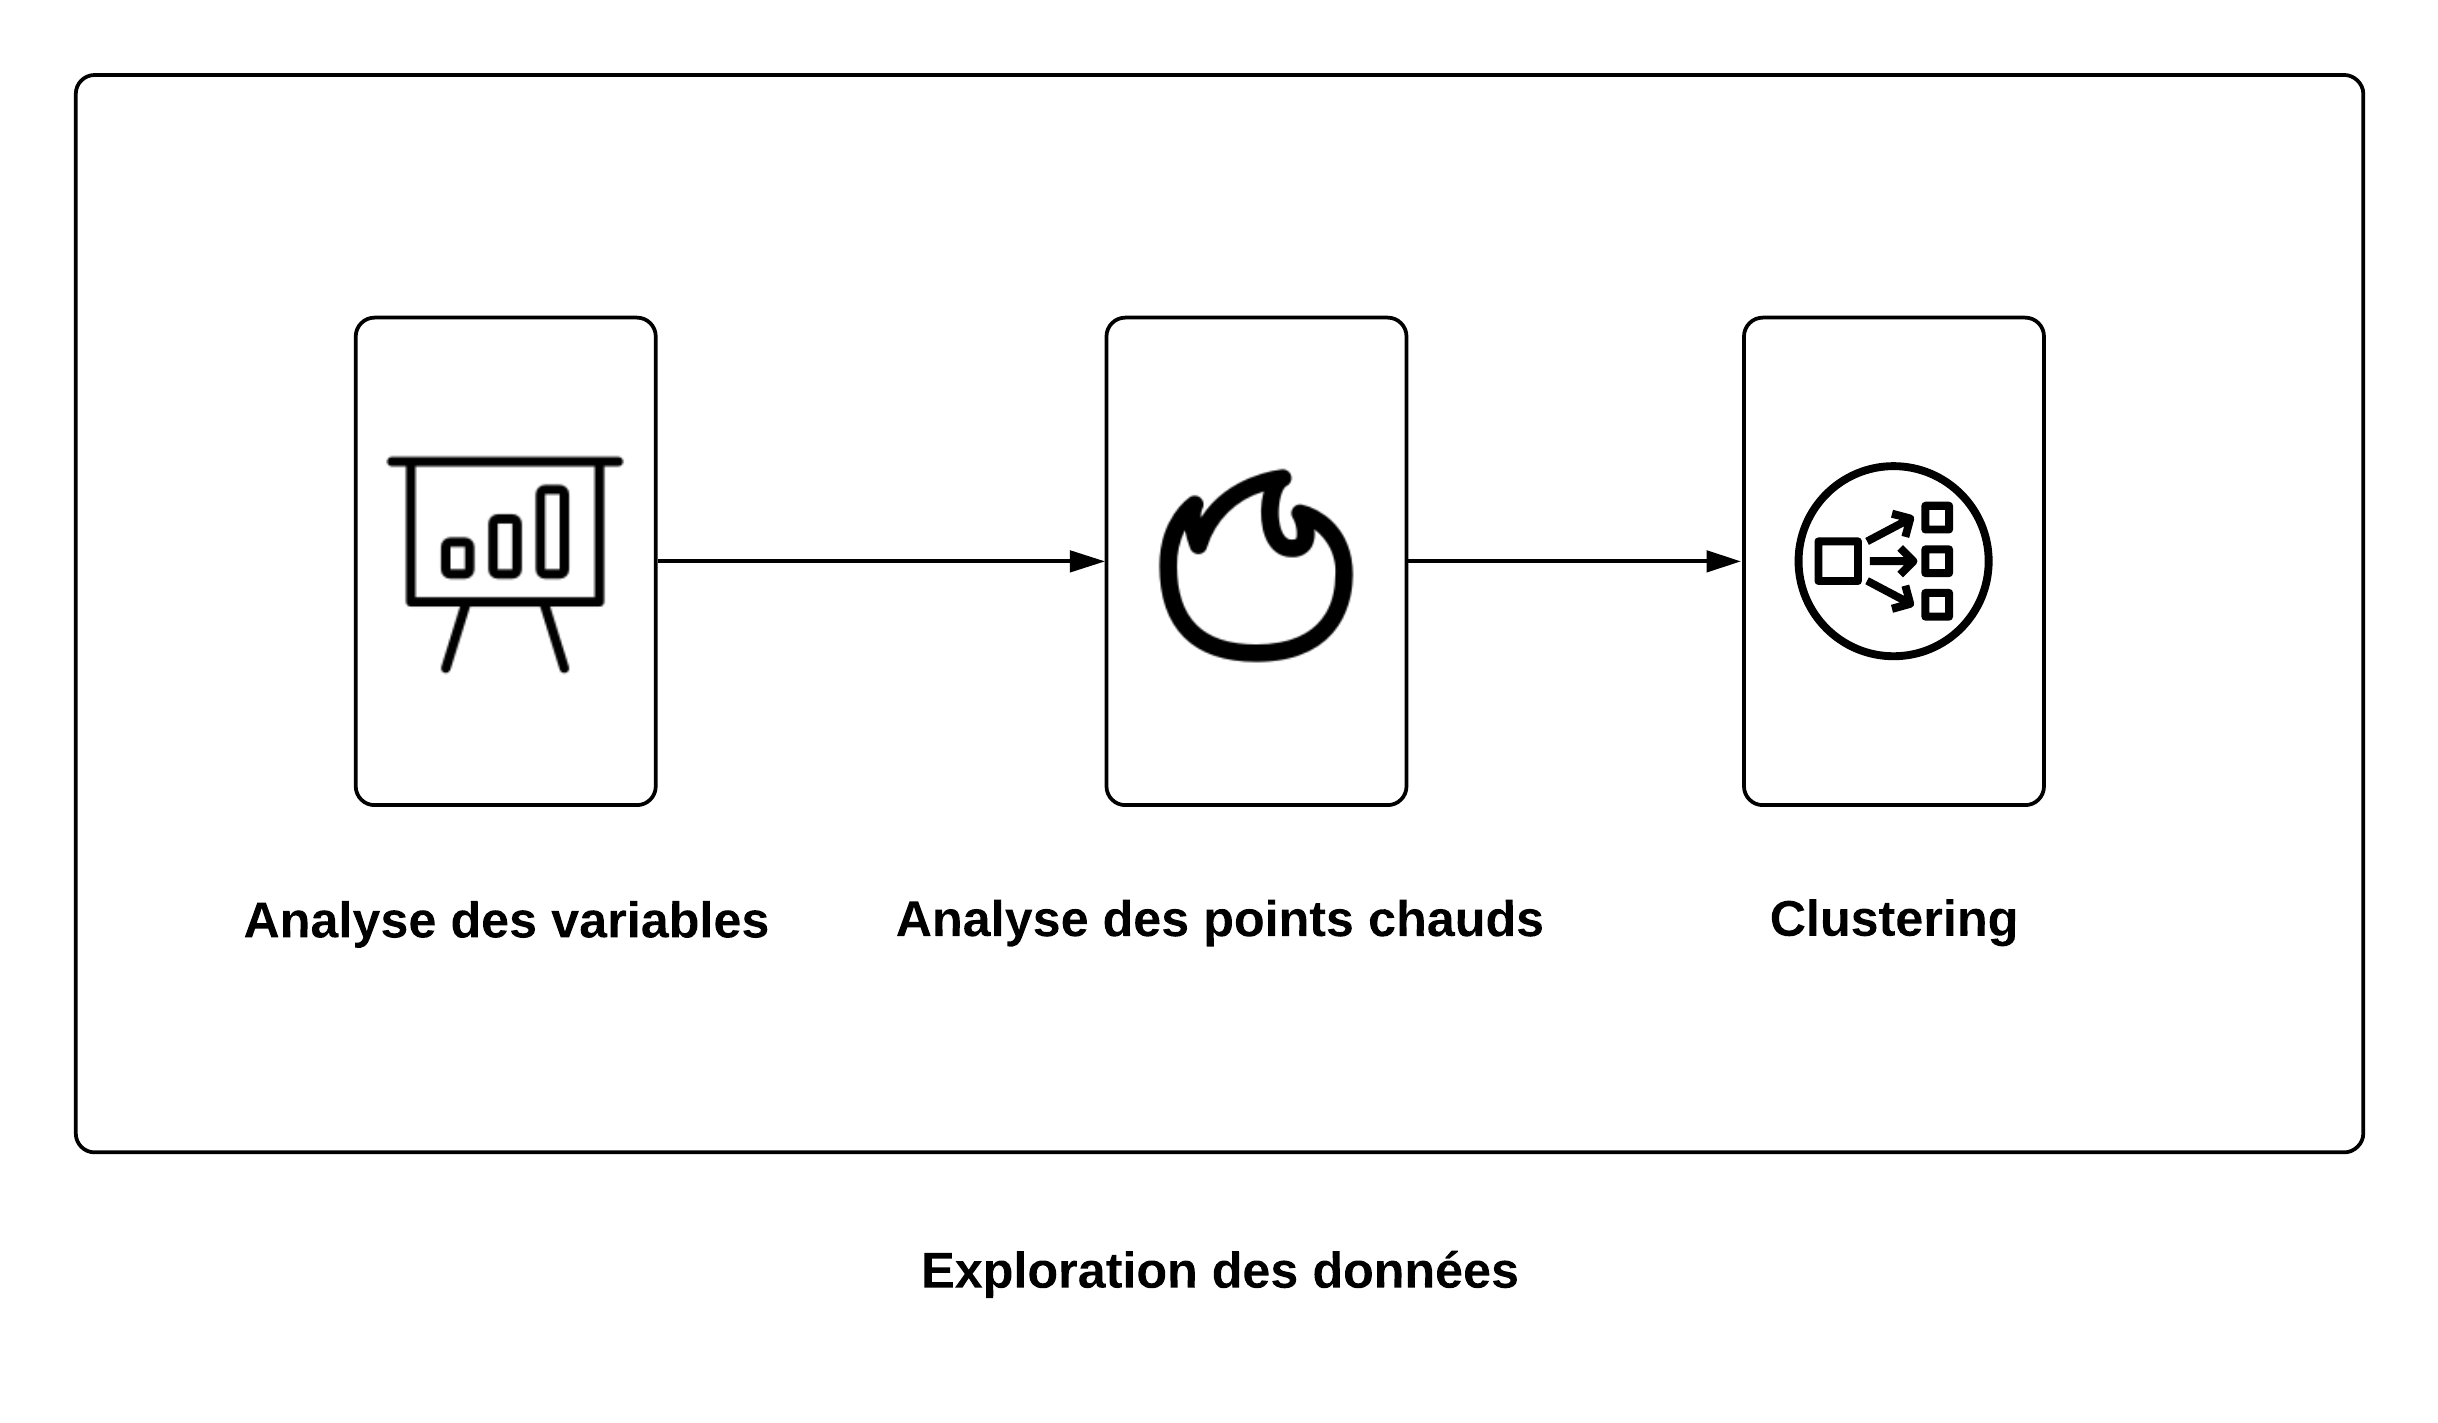
\includegraphics[height=10cm]{images_pfe/DATA_EXPLORATION.png}
  \caption{Les étapes de l'exploration des données}
  \label{fig:data-exploration}
\end{figure}
\FloatBarrier

\subsection{Modélisation}
Lorem ipsum dolor sit amet, consectetur adipiscing elit. Proin posuere euismod neque, non semper nibh viverra sed. Praesent ut varius magna. Fusce ipsum ante, semper nec interdum at, semper et lacus. Nulla ultrices magna a fringilla finibus. Etiam sollicitudin blandit ante. Vivamus blandit rhoncus tincidunt. Morbi sit amet congue purus. Praesent interdum gravida congue. Donec fermentum dui fermentum maximus rutrum.Lorem ipsum dolor sit amet, consectetur adipiscing elit. Proin posuere euismod neque, non semper nibh viverra sed. Praesent ut varius magna. Fusce ipsum ante, semper nec interdum at, semper et lacus. Nulla ultrices magna a fringilla finibus. Etiam sollicitudin blandit ante. Vivamus blandit rhoncus tincidunt. Morbi sit amet congue purus. Praesent interdum gravida congue. Donec fermentum dui fermentum maximus rutrum.

\begin{figure}[hbt!]
  \centering
  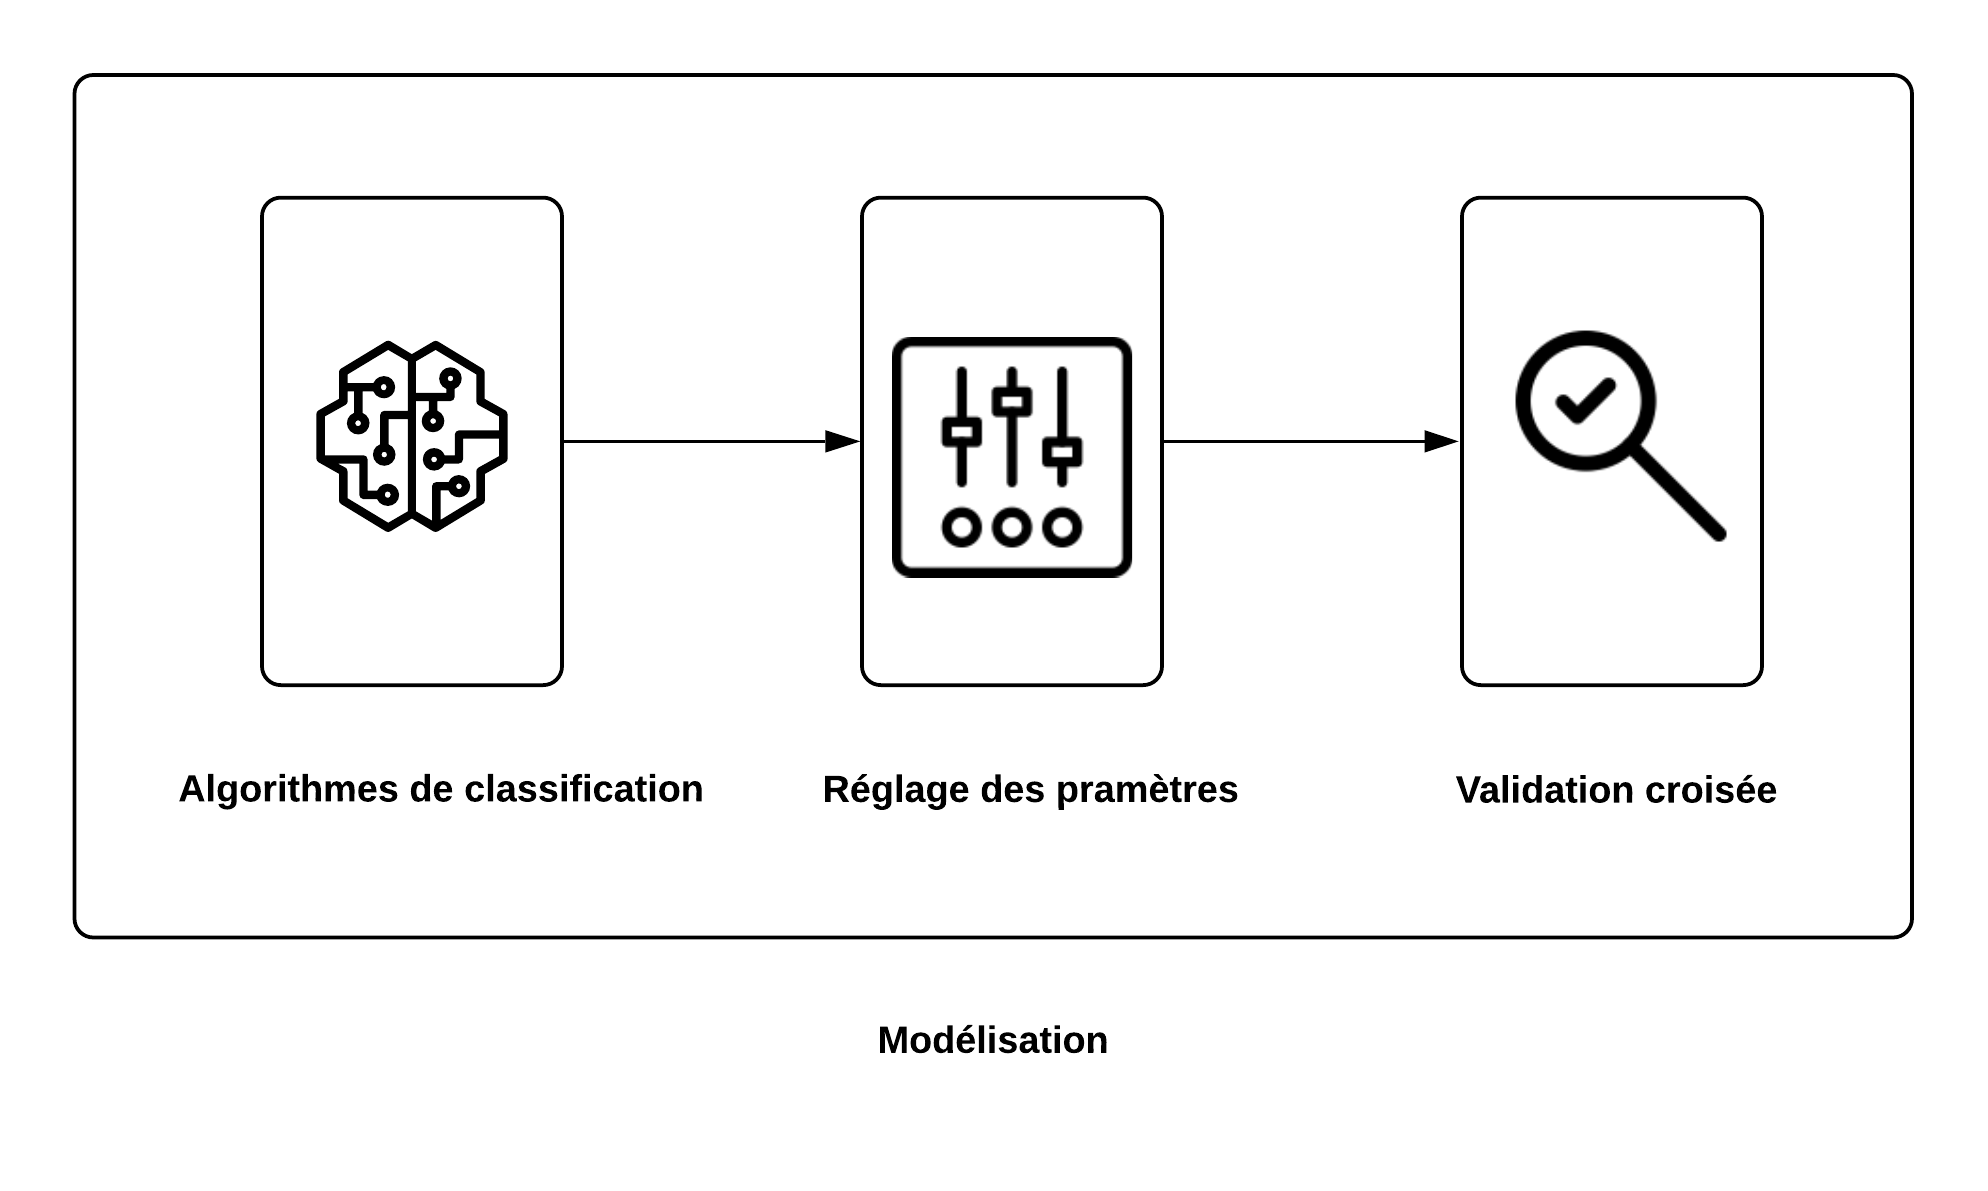
\includegraphics[height=10cm]{images_pfe/DATA_MODELING.png}
  \caption{Les étapes de la modélisation}
  \label{fig:data-modeling}
\end{figure}
\FloatBarrier

\subsection{Élaboration des plans de visite}
Lorem ipsum dolor sit amet, consectetur adipiscing elit. Proin posuere euismod neque, non semper nibh viverra sed. Praesent ut varius magna. Fusce ipsum ante, semper nec interdum at, semper et lacus. Nulla ultrices magna a fringilla finibus. Etiam sollicitudin blandit ante. Vivamus blandit rhoncus tincidunt. Morbi sit amet congue purus. Praesent interdum gravida congue. Donec fermentum dui fermentum maximus rutrum.Lorem ipsum dolor sit amet, consectetur adipiscing elit. Proin posuere euismod neque, non semper nibh viverra sed. Praesent ut varius magna. Fusce ipsum ante, semper nec interdum at, semper et lacus. Nulla ultrices magna a fringilla finibus. Etiam sollicitudin blandit ante. Vivamus blandit rhoncus tincidunt. Morbi sit amet congue purus. Praesent interdum gravida congue. Donec fermentum dui fermentum maximus rutrum. (Voir section \ref{sec:ptsp}).

\medskip
Afin de modéliser le problème mathématiquement, nous utilisons la notation de \parencite{cordeau_tabu_1997} adaptée au PTSP. Soient :

\begin{itemize}
    \item $G = (V, E)$ un graphe complet, où $V = \{0,...,N\}$ est l'ensemble des points de vente à visiter avec $0$ comme point de départ de l'animateur, et $E = V × V$ l'ensemble des arêtes reliant chaque paire de points dans $V$.
    \item $C = (c_{ij})$ la matrice de coût associée à $E$, telle que $c_{ij}$ est la distance entre le point $i$ et le point $j$.
    \item $K = \{1,...,M\}$ l'ensemble des jours de la période.
    \item $R_i$ l'ensemble des combinaisons de visites possibles du point de vente $i$.
    \item $x_{ijk}$ une variable binaire égale à $1$ si et seulement si l'arête $(i,j) \in E$ $(i \ne j)$ figure dans le tour du jour $k \in K$ , 0 sinon.
    \item $y_{ir}$ une variable binaire égale à $1$ si et seulement si la combinaison de visites $r$ est choisi pour le point de vente $i$, 0 sinon.
    \item $a_{rk}$ une constante égale à $1$ si et seulement si le jour $k \in K$ appartient à la combinaison $r \in R_i$.
\end{itemize}

La fonction objectif à minimiser est donnée par l'expression suivante :

\begin{equation*}
    min \sum_{k=1}^M \sum_{(i,j) \in E} c_{ij}x_{ijk}
\end{equation*}

sous les contraintes :

\begin{equation}
    \sum_{r \in R_i} y_{ir} = 1, \  \forall i \in V
    \label{eqn:one-feasible-visit-combination}
\end{equation}

\begin{equation}
    \sum_{j=0}^N x_{ijk} - \sum_{r \in R_i} a_{rk}y_{ir} = 0, \ \forall i \in V, \ \forall k \in K
    \label{eqn:all-visit-combination-days}
\end{equation}

\begin{equation}
    \sum_{(i,j) \in E} x_{ijk} \geqslant 2, \ \forall k \in K
    \label{eqn:one-visit-at-least}
\end{equation}

\begin{equation}
    \sum_{i,j \in S} x_{ijk} \leq |S| - 1, \ \forall k \in K, \ \forall S \subseteq V \setminus \{0\} , \ \textrm{avec} \ |S| \geqslant 2
    \label{eqn:no-subtours}
\end{equation}

\begin{equation}
    x_{ijk} \in \{0,1\}, \ \forall i,j \in V, \ \forall k \in K 
\end{equation}

\begin{equation}
    y_{ir} \in \{0,1\}, \ \forall i \in V, \ \forall r \in R_i
\end{equation}

La contrainte (\ref{eqn:one-feasible-visit-combination}) garantit qu'une et une seule combinaison de visites est attribuée à chaque point de vente, tandis que la contrainte (\ref{eqn:all-visit-combination-days}) garantit que les visites se font seulement les jours de la combinaison attribuée. la contrainte (\ref{eqn:one-visit-at-least}) garantit qu'au mois une visite est faite chaque jour (en comptabilisant le point de départ). (\ref{eqn:no-subtours}) est une contrainte d'élimination des sous-tours.


\begin{figure}[hbt!]
  \centering
  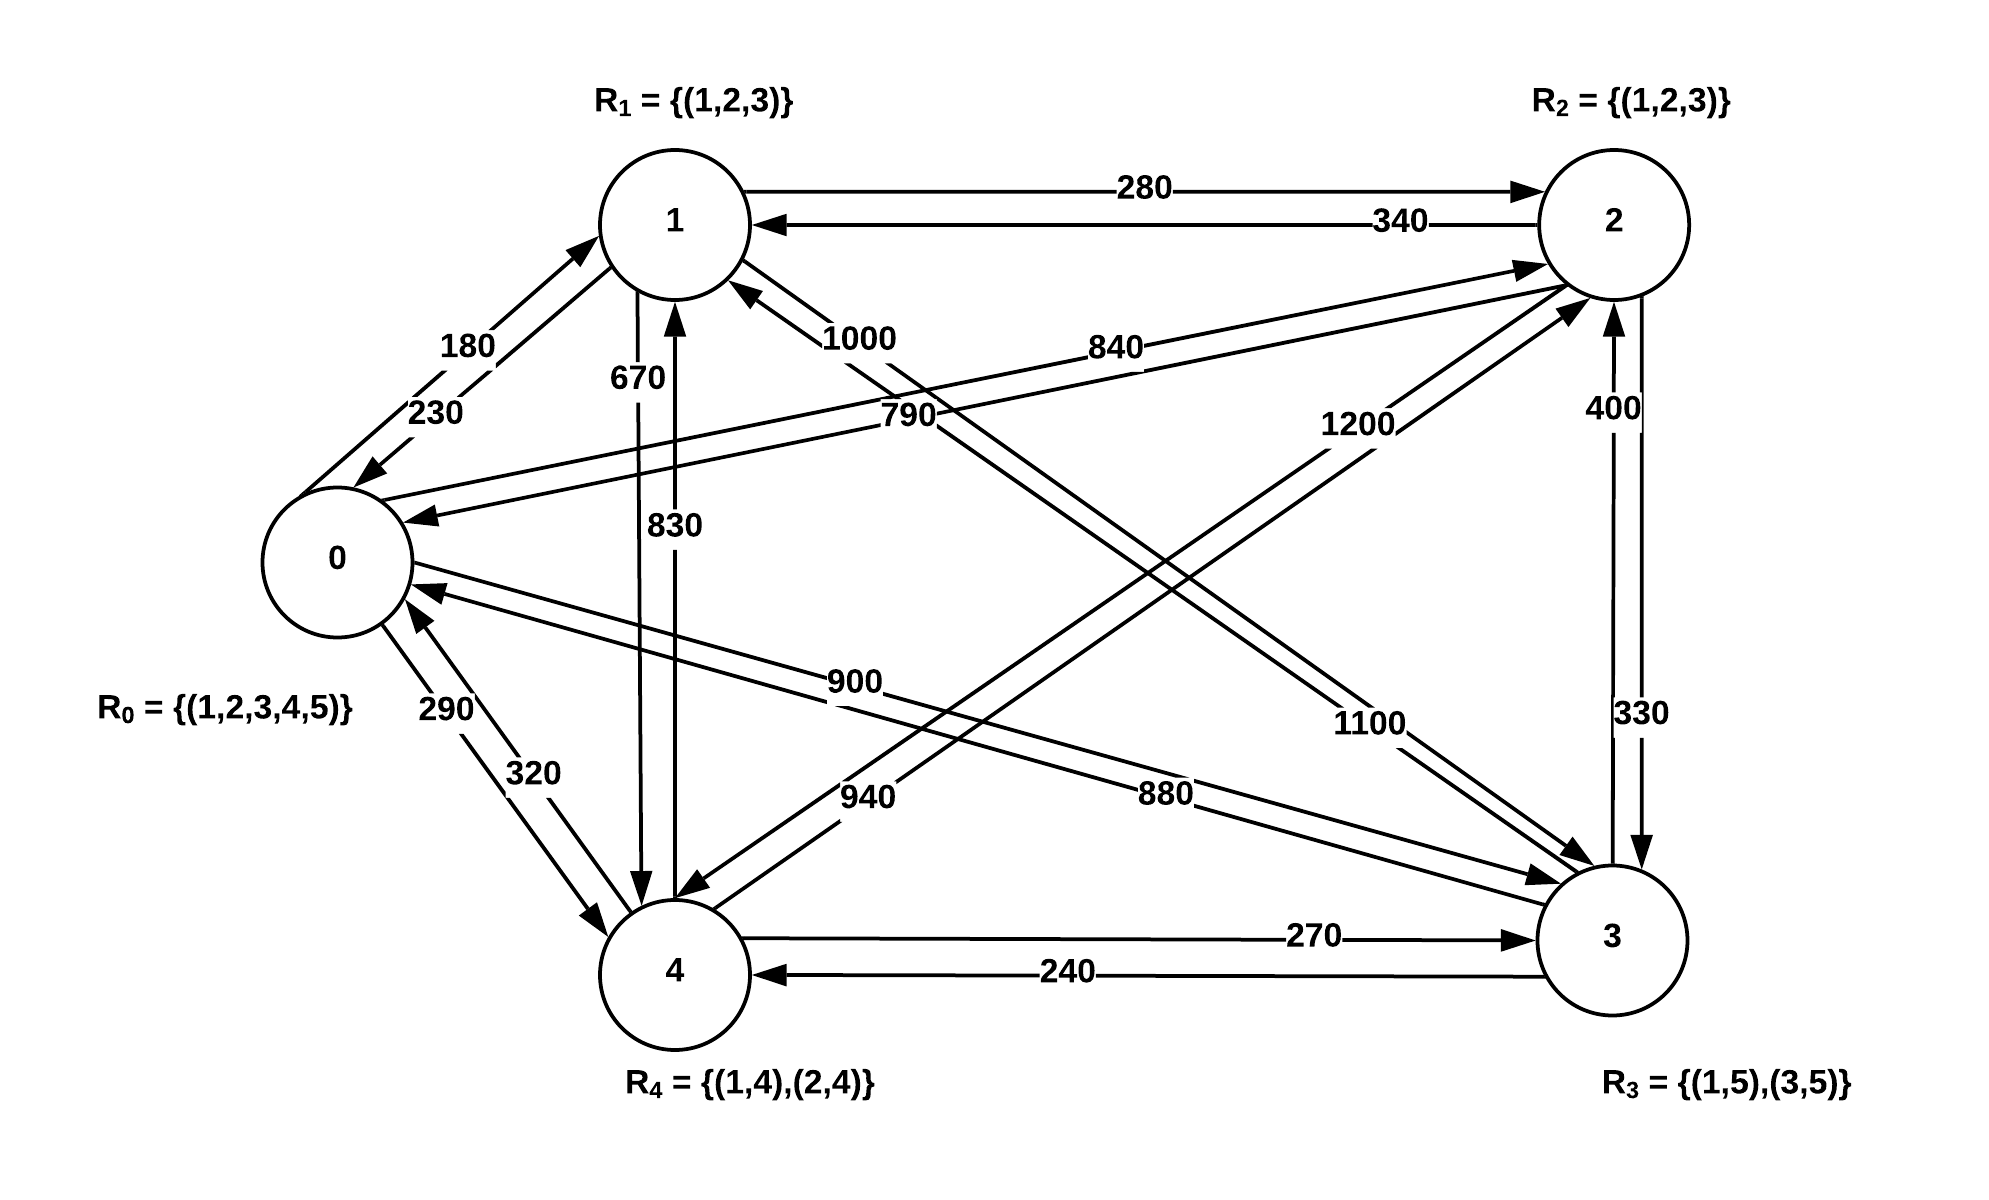
\includegraphics[height=10cm]{images_pfe/PTSP_EXAMPLE.png}
  \caption{Exemple d'un PTSP avec un point de départ et quatre points de vente sur une période de 5 jours. Les $R_i$ représentent les combinaisons de visites et les chiffres sur les arcs représentent les coûts. Exemple : le noeud 4 peut être visité soit les jours 1 et 4 ou les jours 2 et 4.}
  \label{fig:ptsp-example}
\end{figure}
\FloatBarrier

\medskip
Lorem ipsum dolor sit amet, consectetur adipiscing elit. Proin posuere euismod neque, non semper nibh viverra sed. Praesent ut varius magna. Fusce ipsum ante, semper nec interdum at, semper et lacus. Nulla ultrices magna a fringilla finibus. Etiam sollicitudin blandit ante. Vivamus blandit rhoncus tincidunt. Morbi sit amet congue purus. Praesent interdum gravida congue. Donec fermentum dui fermentum maximus rutrum. \parencite{hemmelmayr_variable_2009} (Voir \ref{sub-sec:hdh}) Lorem ipsum dolor sit amet, consectetur adipiscing elit. Proin posuere euismod neque, non semper nibh viverra sed. Praesent ut varius magna. Fusce ipsum ante, semper nec interdum at, semper et lacus. Nulla ultrices magna a fringilla finibus. Etiam sollicitudin blandit ante. Vivamus blandit rhoncus tincidunt. Morbi sit amet congue purus. Praesent interdum gravida congue. Donec fermentum dui fermentum maximus rutrum.

Lorem ipsum dolor sit amet, consectetur adipiscing elit. Proin posuere euismod neque, non semper nibh viverra sed. Praesent ut varius magna. Fusce ipsum ante, semper nec interdum at, semper et lacus. Nulla ultrices magna a fringilla finibus. Etiam sollicitudin blandit ante. Vivamus blandit rhoncus tincidunt. Morbi sit amet congue purus. Praesent interdum gravida congue. Donec fermentum dui fermentum maximus rutrum. (Voir algorithme \ref{alg:initial-solution}). Lorem ipsum dolor sit amet, consectetur adipiscing elit. Proin posuere euismod neque, non semper nibh viverra sed. Praesent ut varius magna. Fusce ipsum ante, semper nec interdum at, semper et lacus. Nulla ultrices magna a fringilla finibus. Etiam sollicitudin blandit ante. Vivamus blandit rhoncus tincidunt. Morbi sit amet congue purus. Praesent interdum gravida congue. Donec fermentum dui fermentum maximus rutrum. (Voir \ref{par:nn}).

\medskip

\begin{algorithm}[H]
  \KwIn{period, point\_of\_sales, visit\_combinations}
  \KwOut{routes}
  routes $\gets$ EmptyRoutes(period) \;
  \ForEach{ \textup{pos} $\in$ \textup{point\_of\_sales} }{
    combination $\gets$ choose random visit combination from pos combinations \;
    \ForEach{ \textup{day} $\in$ \textup{combination} }{
        add pos to routes[day]  \;
    }
  }
  \ForEach{\textup{day} $\in$ \textup{period}}{
    apply nearest neighbour heuristic on routes[day]  \;
  }
  \Return routes \;
  \caption{Initial Solution}
  \label{alg:initial-solution}
\end{algorithm}
\FloatBarrier

\medskip

Lorem ipsum dolor sit amet, consectetur adipiscing elit. Proin posuere euismod neque, non semper nibh viverra sed. Praesent ut varius magna. Fusce ipsum ante, semper nec interdum at, semper et lacus. Nulla ultrices magna a fringilla finibus. Etiam sollicitudin blandit ante. Vivamus blandit rhoncus tincidunt. Morbi sit amet congue purus. Praesent interdum gravida congue. Donec fermentum dui fermentum maximus rutrum.(Voir figure \ref{fig:shake-combinations}). Lorem ipsum dolor sit amet, consectetur adipiscing elit. Proin posuere euismod neque, non semper nibh viverra sed. Praesent ut varius magna. Fusce ipsum ante, semper nec interdum at, semper et lacus. Nulla ultrices magna a fringilla finibus. Etiam sollicitudin blandit ante. Vivamus blandit rhoncus tincidunt. Morbi sit amet congue purus. Praesent interdum gravida congue. Donec fermentum dui fermentum maximus rutrum. (Voir figure \ref{fig:shake-route}). Lorem ipsum dolor sit amet, consectetur adipiscing elit. Proin posuere euismod neque, non semper nibh viverra sed. Praesent ut varius magna. Fusce ipsum ante, semper nec interdum at, semper et lacus. Nulla ultrices magna a fringilla finibus. Etiam sollicitudin blandit ante. Vivamus blandit rhoncus tincidunt. Morbi sit amet congue purus. Praesent interdum gravida congue. Donec fermentum dui fermentum maximus rutrum. (Voir algorithme \ref{alg:local-search}).

\medskip

\begin{algorithm}[H]
  \KwIn{routes, visit\_combinations, MAX\_ITERATIONS}
  \KwOut{best\_routes}
  best\_routes $\gets$ routes \;
  \For{\textup{(i=0; i < MAX\_ITERATIONS; i++)} }{
    routes $\gets$ shake visit combinations \;
    routes $\gets$ shake routes \;
    routes $\gets$ apply 2-opt \;
    \eIf{\textup{routes is better than best\_routes or an acceptance citeria is met}}{
        best\_routes $\gets$ routes \;
    }{
    routes $\gets$ best\_routes \;
    }
    
  }
  
  \Return best\_routes \;
  \caption{Local Search}
  \label{alg:local-search}
\end{algorithm}
\FloatBarrier

\medskip

\begin{figure}[hbt!]
  \centering
  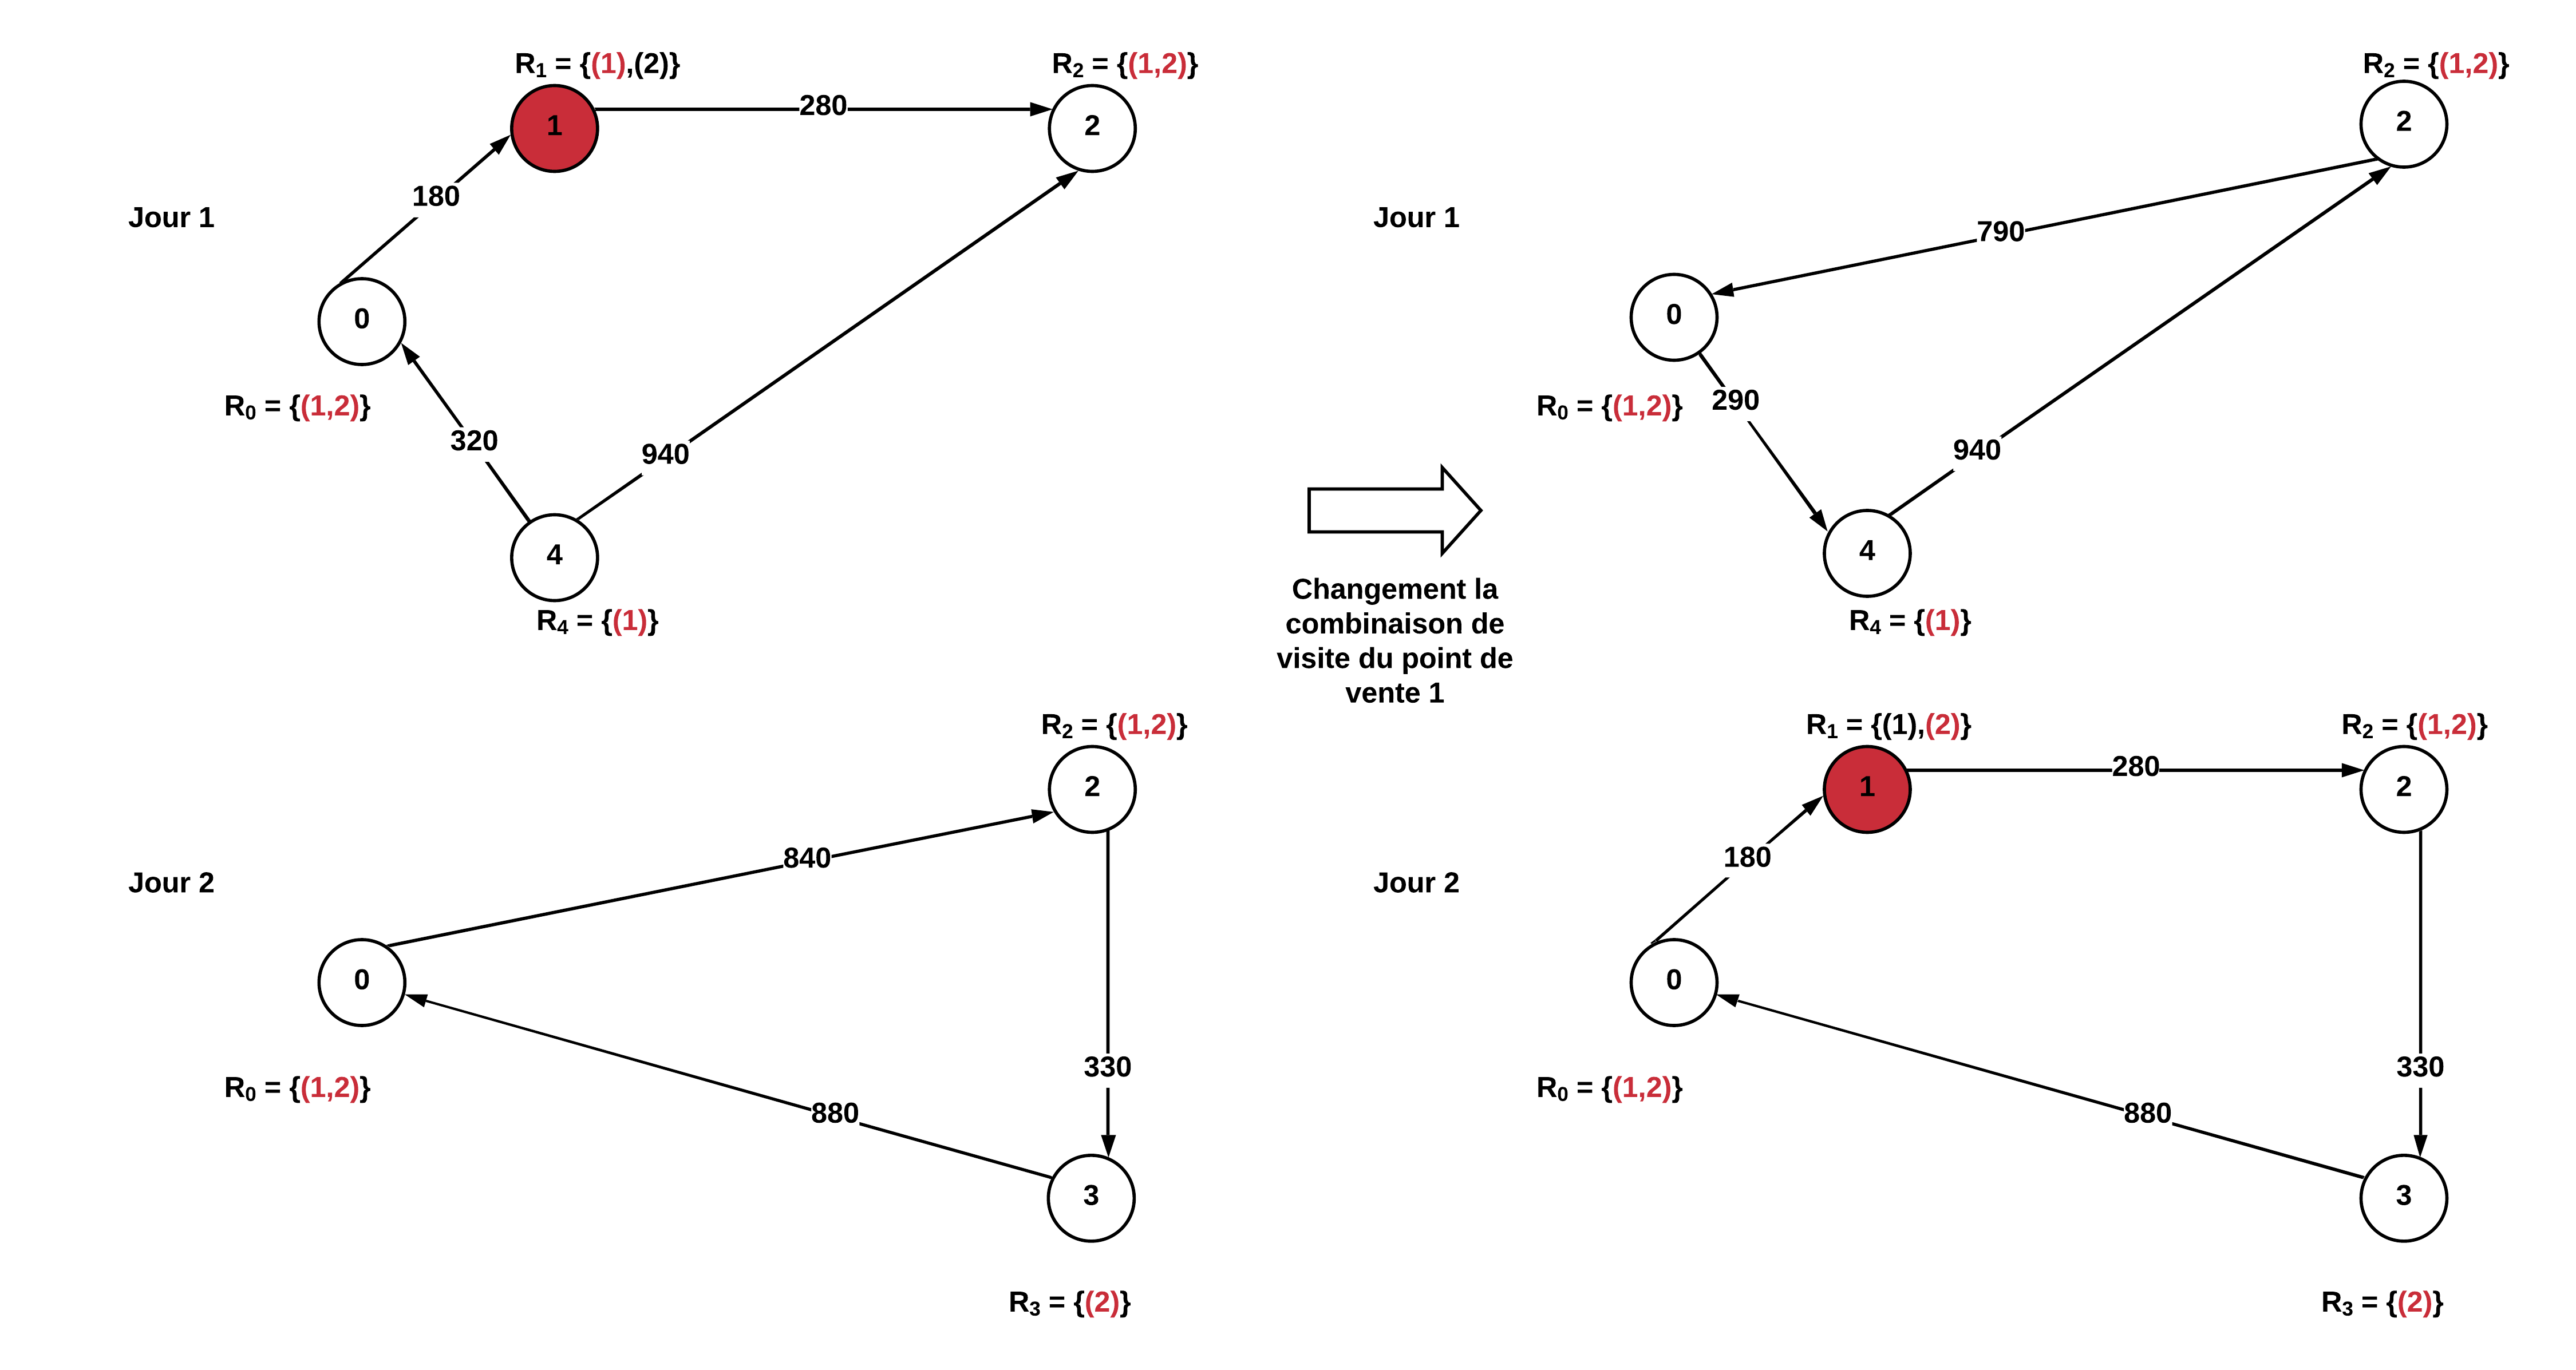
\includegraphics[width=16cm]{images_pfe/SHAKE_COMBINATIONS.png}
  \caption{Exemple d'un changement de combinaison de visites sur une période de 2 jours.}
  \label{fig:shake-combinations}
\end{figure}
\FloatBarrier

\medskip

\begin{figure}[hbt!]
  \centering
  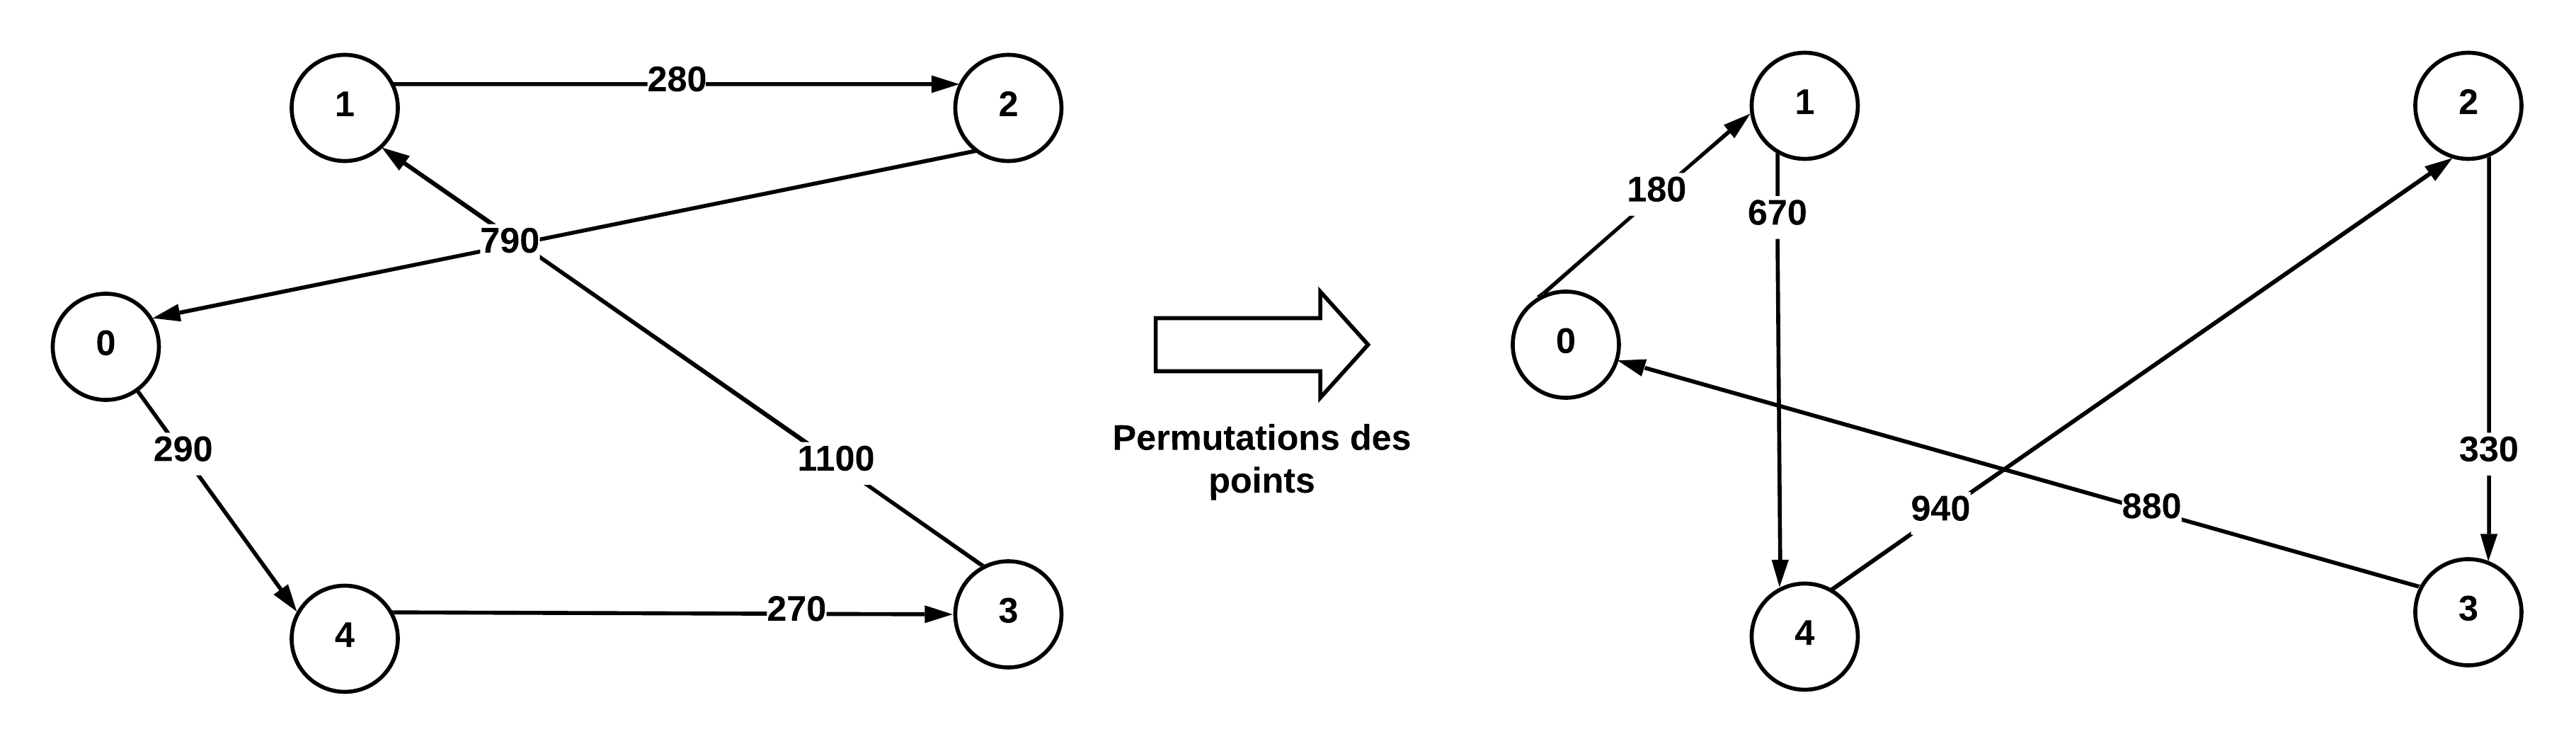
\includegraphics[width=16cm]{images_pfe/SHAKE_ROUTES.png}
  \caption{Exemple de perturbation d'une route.}
  \label{fig:shake-route}
\end{figure}
\FloatBarrier

\medskip
Lorem ipsum dolor sit amet, consectetur adipiscing elit. Proin posuere euismod neque, non semper nibh viverra sed. Praesent ut varius magna. Fusce ipsum ante, semper nec interdum at, semper et lacus. Nulla ultrices magna a fringilla finibus. Etiam sollicitudin blandit ante. Vivamus blandit rhoncus tincidunt. Morbi sit amet congue purus. Praesent interdum gravida congue. Donec fermentum dui fermentum maximus rutrum.\parencite{hemmelmayr_variable_2009}. Lorem ipsum dolor sit amet, consectetur adipiscing elit. Proin posuere euismod neque, non semper nibh viverra sed. Praesent ut varius magna. Fusce ipsum ante, semper nec interdum at, semper et lacus. Nulla ultrices magna a fringilla finibus. Etiam sollicitudin blandit ante. Vivamus blandit rhoncus tincidunt. Morbi sit amet congue purus. Praesent interdum gravida congue. Donec fermentum dui fermentum maximus rutrum.e :
\begin{equation*}
    P(x') = \exp{\frac{-(f(x')-f(x))}{T}}
\end{equation*}
 Où $f(x')$ et $f(x)$ représentent les coûts de la solution voisine $x'$ et la solution courante $x$, respectivement, et $T$ est une température diminuée linéairement au cours de la recherche. Lorem ipsum dolor sit amet, consectetur adipiscing elit. Proin posuere euismod neque, non semper nibh viverra sed. Praesent ut varius magna. Fusce ipsum ante, semper nec interdum at, semper et lacus. Nulla ultrices magna a fringilla finibus. Etiam sollicitudin blandit ante. Vivamus blandit rhoncus tincidunt. Morbi sit amet congue purus. Praesent interdum gravida congue. Donec fermentum dui fermentum maximus rutrum..

\subsection{Synchronisation des plans de visite en temps réel}

Lorem ipsum dolor sit amet, consectetur adipiscing elit. Proin posuere euismod neque, non semper nibh viverra sed. Praesent ut varius magna. Fusce ipsum ante, semper nec interdum at, semper et lacus. Nulla ultrices magna a fringilla finibus. Etiam sollicitudin blandit ante. Vivamus blandit rhoncus tincidunt. Morbi sit amet congue purus. Praesent interdum gravida congue. Donec fermentum dui fermentum maximus rutrum. (Voir \ref{par:lin-kernighan} ) et est décrite dans les papiers \parencite{helsgaun_effective_2000,helsgaun_general_2009}. Lorem ipsum dolor sit amet, consectetur adipiscing elit. Proin posuere euismod neque, non semper nibh viverra sed. Praesent ut varius magna. Fusce ipsum ante, semper nec interdum at, semper et lacus. Nulla ultrices magna a fringilla finibus. Etiam sollicitudin blandit ante. Vivamus blandit rhoncus tincidunt. Morbi sit amet congue purus. Praesent interdum gravida congue. Donec fermentum dui fermentum maximus rutrum. (Voir algorithme \ref{alg:sync}).

\medskip

\begin{algorithm}[H]
  \KwIn{route}
  \KwOut{updated\_route}
  traffic\_data $\gets$ get real time traffic data \;
  updated\_route $\gets$ LKH(route, traffic\_data) \;
  
  \Return updated\_route \;
  \caption{Route Synchronization}
  \label{alg:sync}
\end{algorithm}
\FloatBarrier

\medskip


\section{Plateforme de visualisation}
Lorem ipsum dolor sit amet, consectetur adipiscing elit. Proin posuere euismod neque, non semper nibh viverra sed. Praesent ut varius magna. Fusce ipsum ante, semper nec interdum at, semper et lacus. Nulla ultrices magna a fringilla finibus. Etiam sollicitudin blandit ante. Vivamus blandit rhoncus tincidunt. Morbi sit amet congue purus. Praesent interdum gravida congue. Donec fermentum dui fermentum maximus rutrum.

\medskip

Lorem ipsum dolor sit amet, consectetur adipiscing elit. Proin posuere euismod neque, non semper nibh viverra sed. Praesent ut varius magna. Fusce ipsum ante, semper nec interdum at, semper et lacus. Nulla ultrices magna a fringilla finibus. Etiam sollicitudin blandit ante. Vivamus blandit rhoncus tincidunt. Morbi sit amet congue purus. Praesent interdum gravida congue. Donec fermentum dui fermentum maximus rutrum. (Voir \ref{app:rest}). Cette Lorem ipsum dolor sit amet, consectetur adipiscing elit. Proin posuere euismod neque, non semper nibh viverra sed. Praesent ut varius magna. Fusce ipsum ante, semper nec interdum at, semper et lacus. Nulla ultrices magna a fringilla finibus. Etiam sollicitudin blandit ante. Vivamus blandit rhoncus tincidunt. Morbi sit amet congue purus. Praesent interdum gravida congue. Donec fermentum dui fermentum maximus rutrum.

\medskip


\begin{figure}[hbt!]
  \centering
  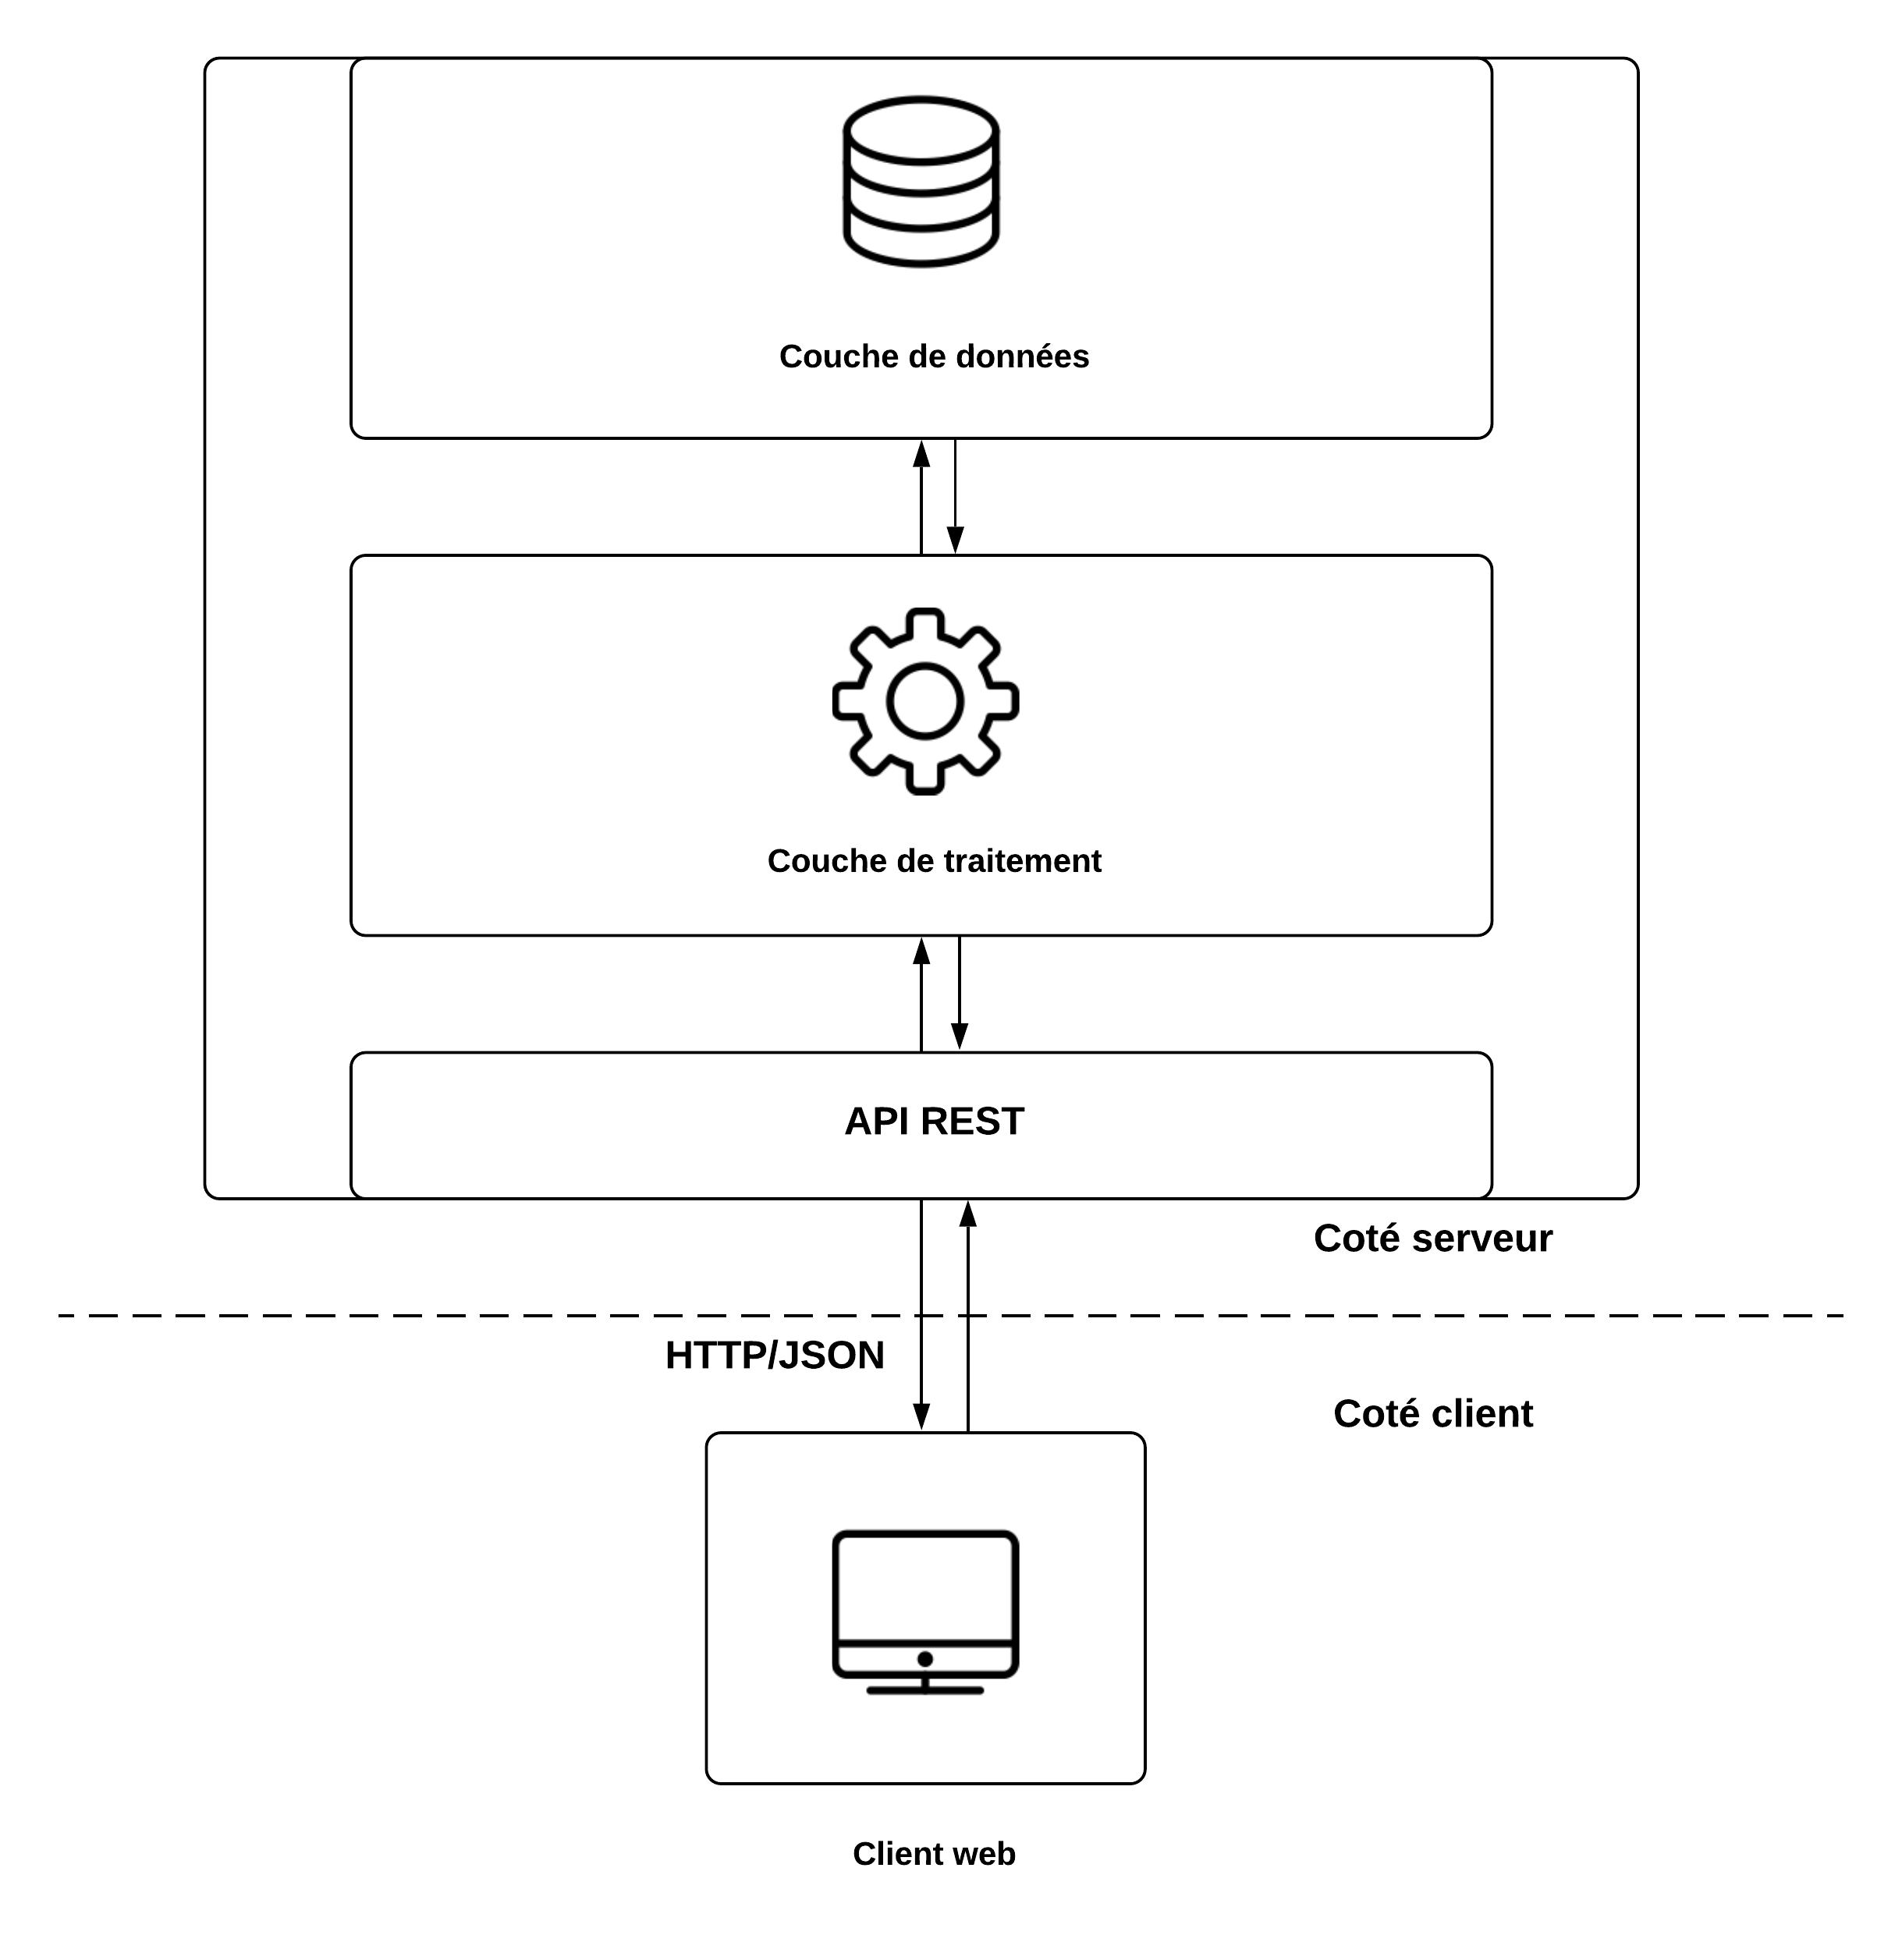
\includegraphics[height=10cm]{images_pfe/VIZ_PLATFORM_ARCHITECTURE.png}
  \caption{Architecture de la plateforme de visualisation.}
  \label{fig:viz-platform-architecture}
\end{figure}
\FloatBarrier

Lorem ipsum dolor sit amet, consectetur adipiscing elit. Proin posuere euismod neque, non semper nibh viverra sed. Praesent ut varius magna. Fusce ipsum ante, semper nec interdum at, semper et lacus. Nulla ultrices magna a fringilla finibus. Etiam sollicitudin blandit ante. Vivamus blandit rhoncus tincidunt. Morbi sit amet congue purus. Praesent interdum gravida congue. Donec fermentum dui fermentum maximus rutrum. (Voir annexe \ref{app:http}).

\begin{figure}[hbt!]
  \centering
  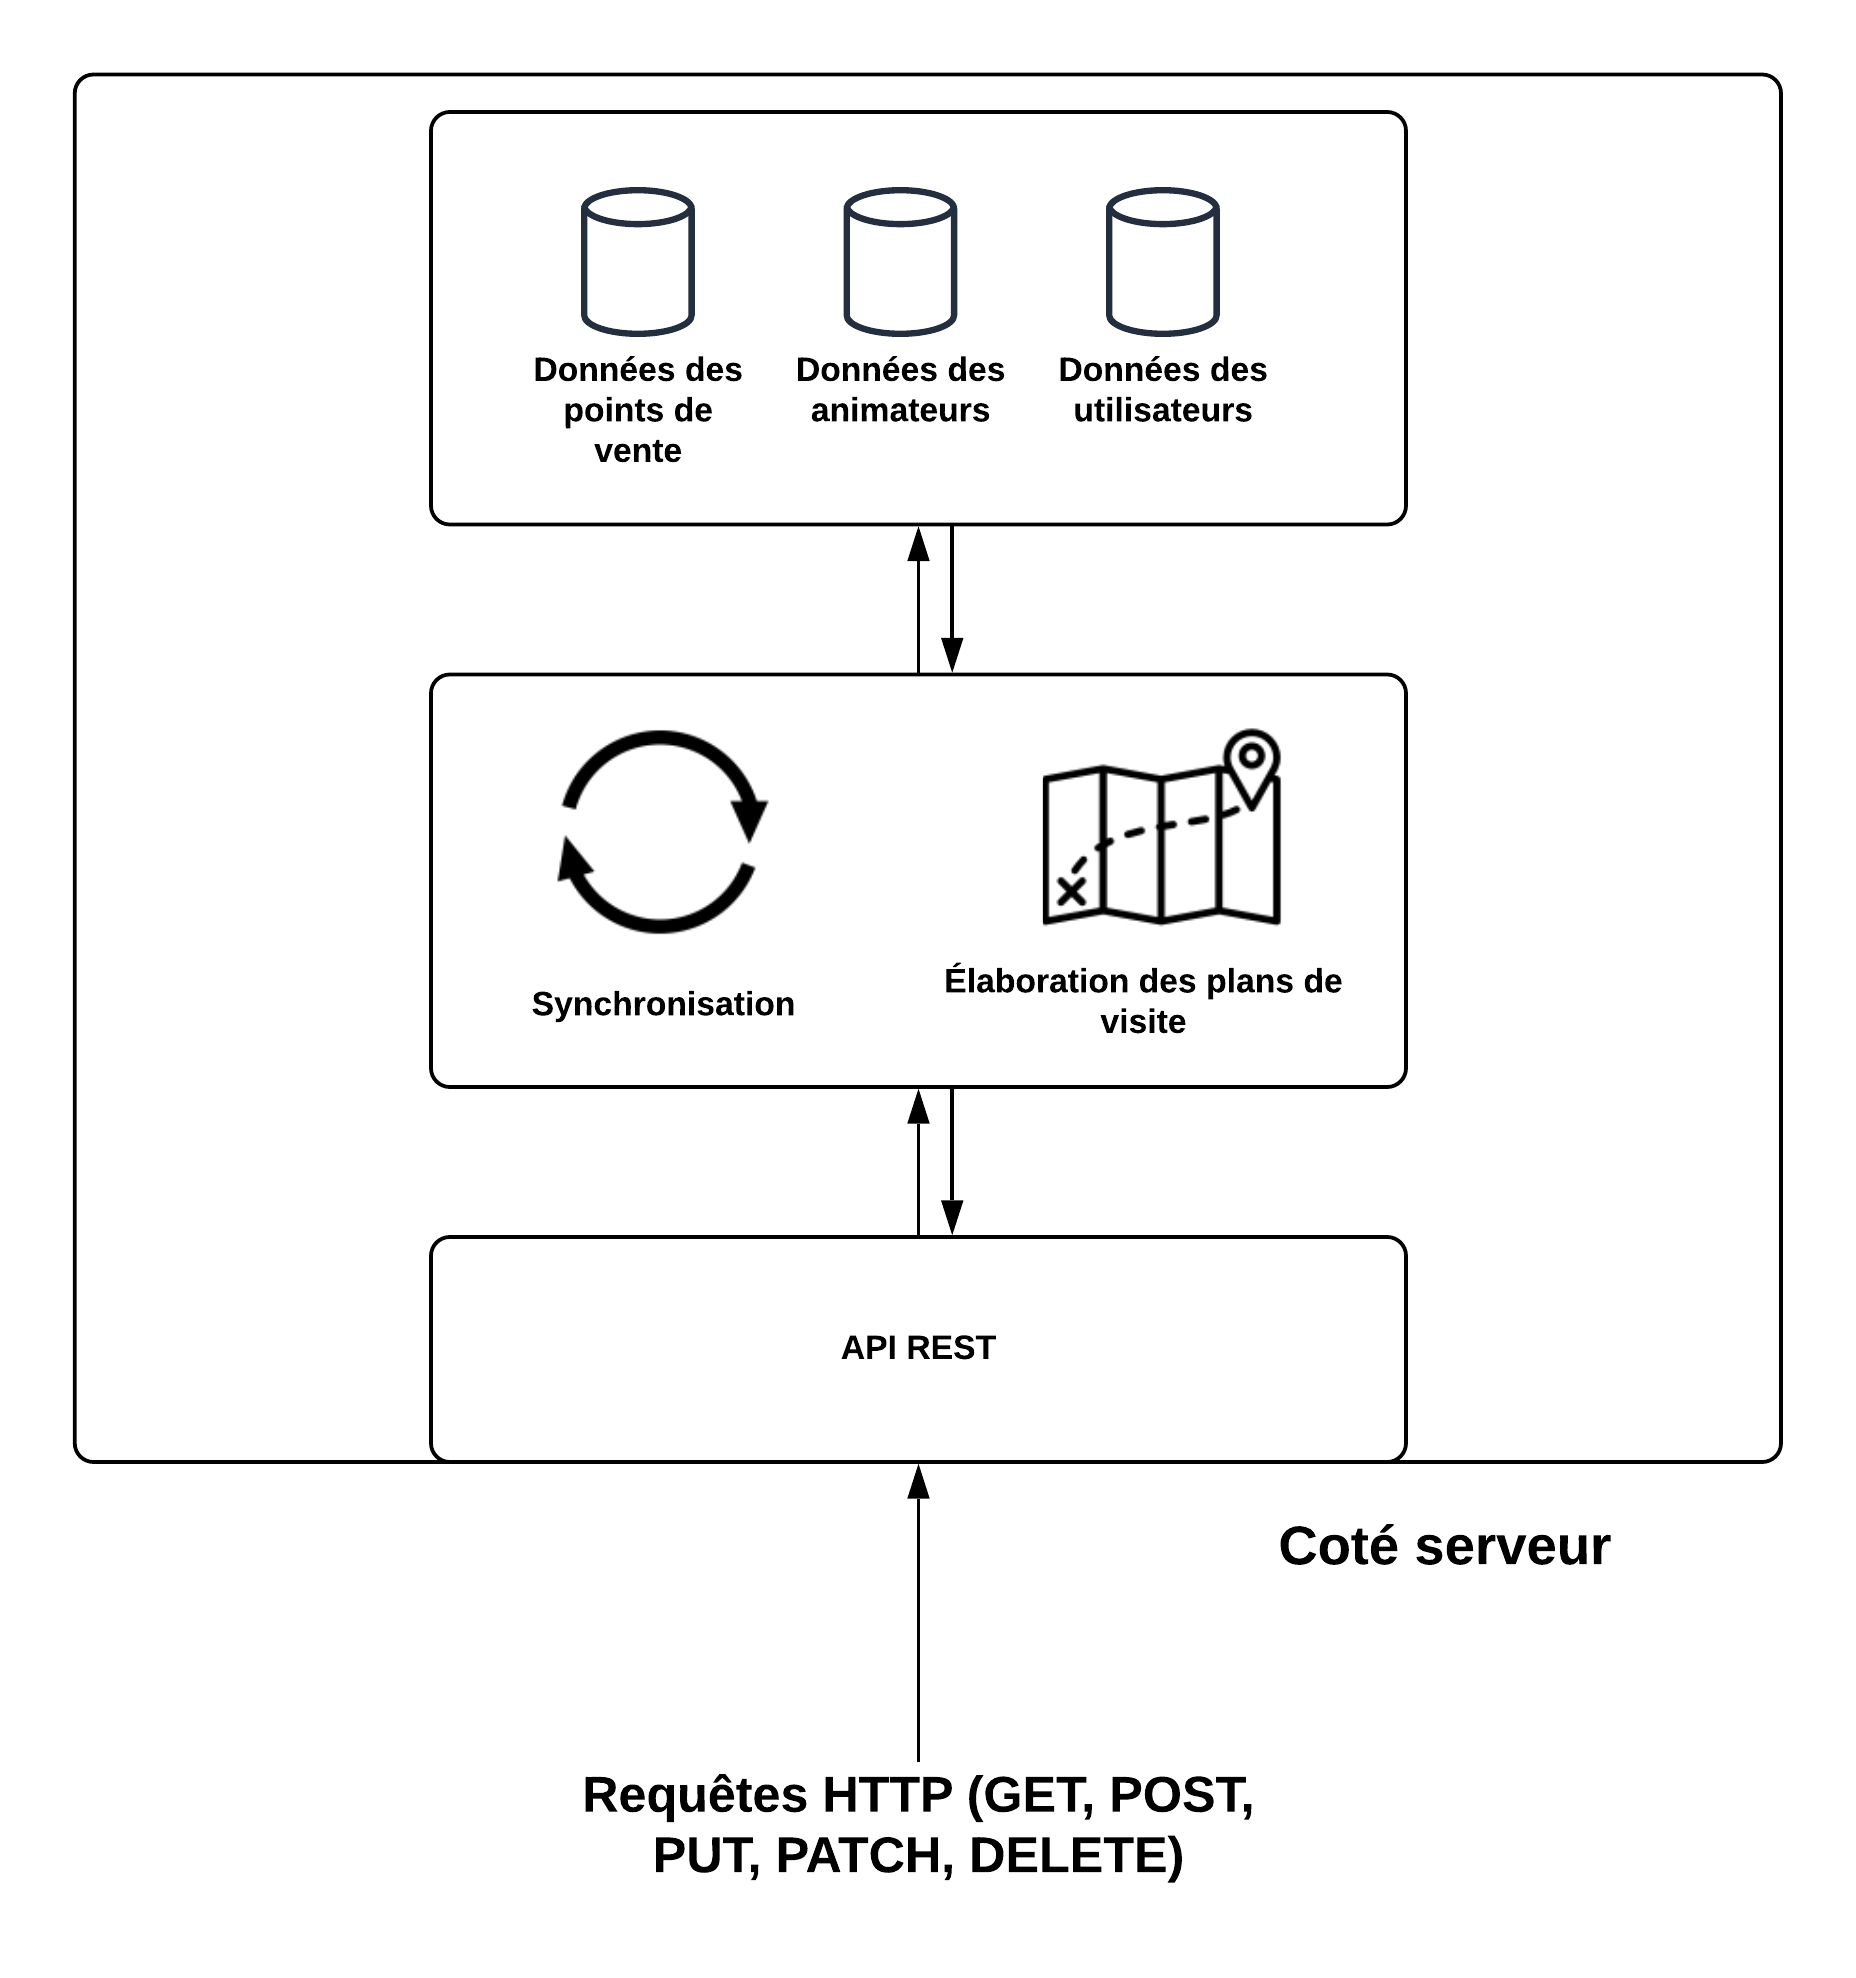
\includegraphics[height=10cm]{images_pfe/SERVER_SIDE.png}
  \caption{Partie serveur.}
  \label{fig:server-side}
\end{figure}
\FloatBarrier

\medskip

Lorem ipsum dolor sit amet, consectetur adipiscing elit. Proin posuere euismod neque, non semper nibh viverra sed. Praesent ut varius magna. Fusce ipsum ante, semper nec interdum at, semper et lacus. Nulla ultrices magna a fringilla finibus. Etiam sollicitudin blandit ante. Vivamus blandit rhoncus tincidunt. Morbi sit amet congue purus. Praesent interdum gravida congue. Donec fermentum dui fermentum maximus rutrum.


\begin{figure}[hbt!]
  \centering
  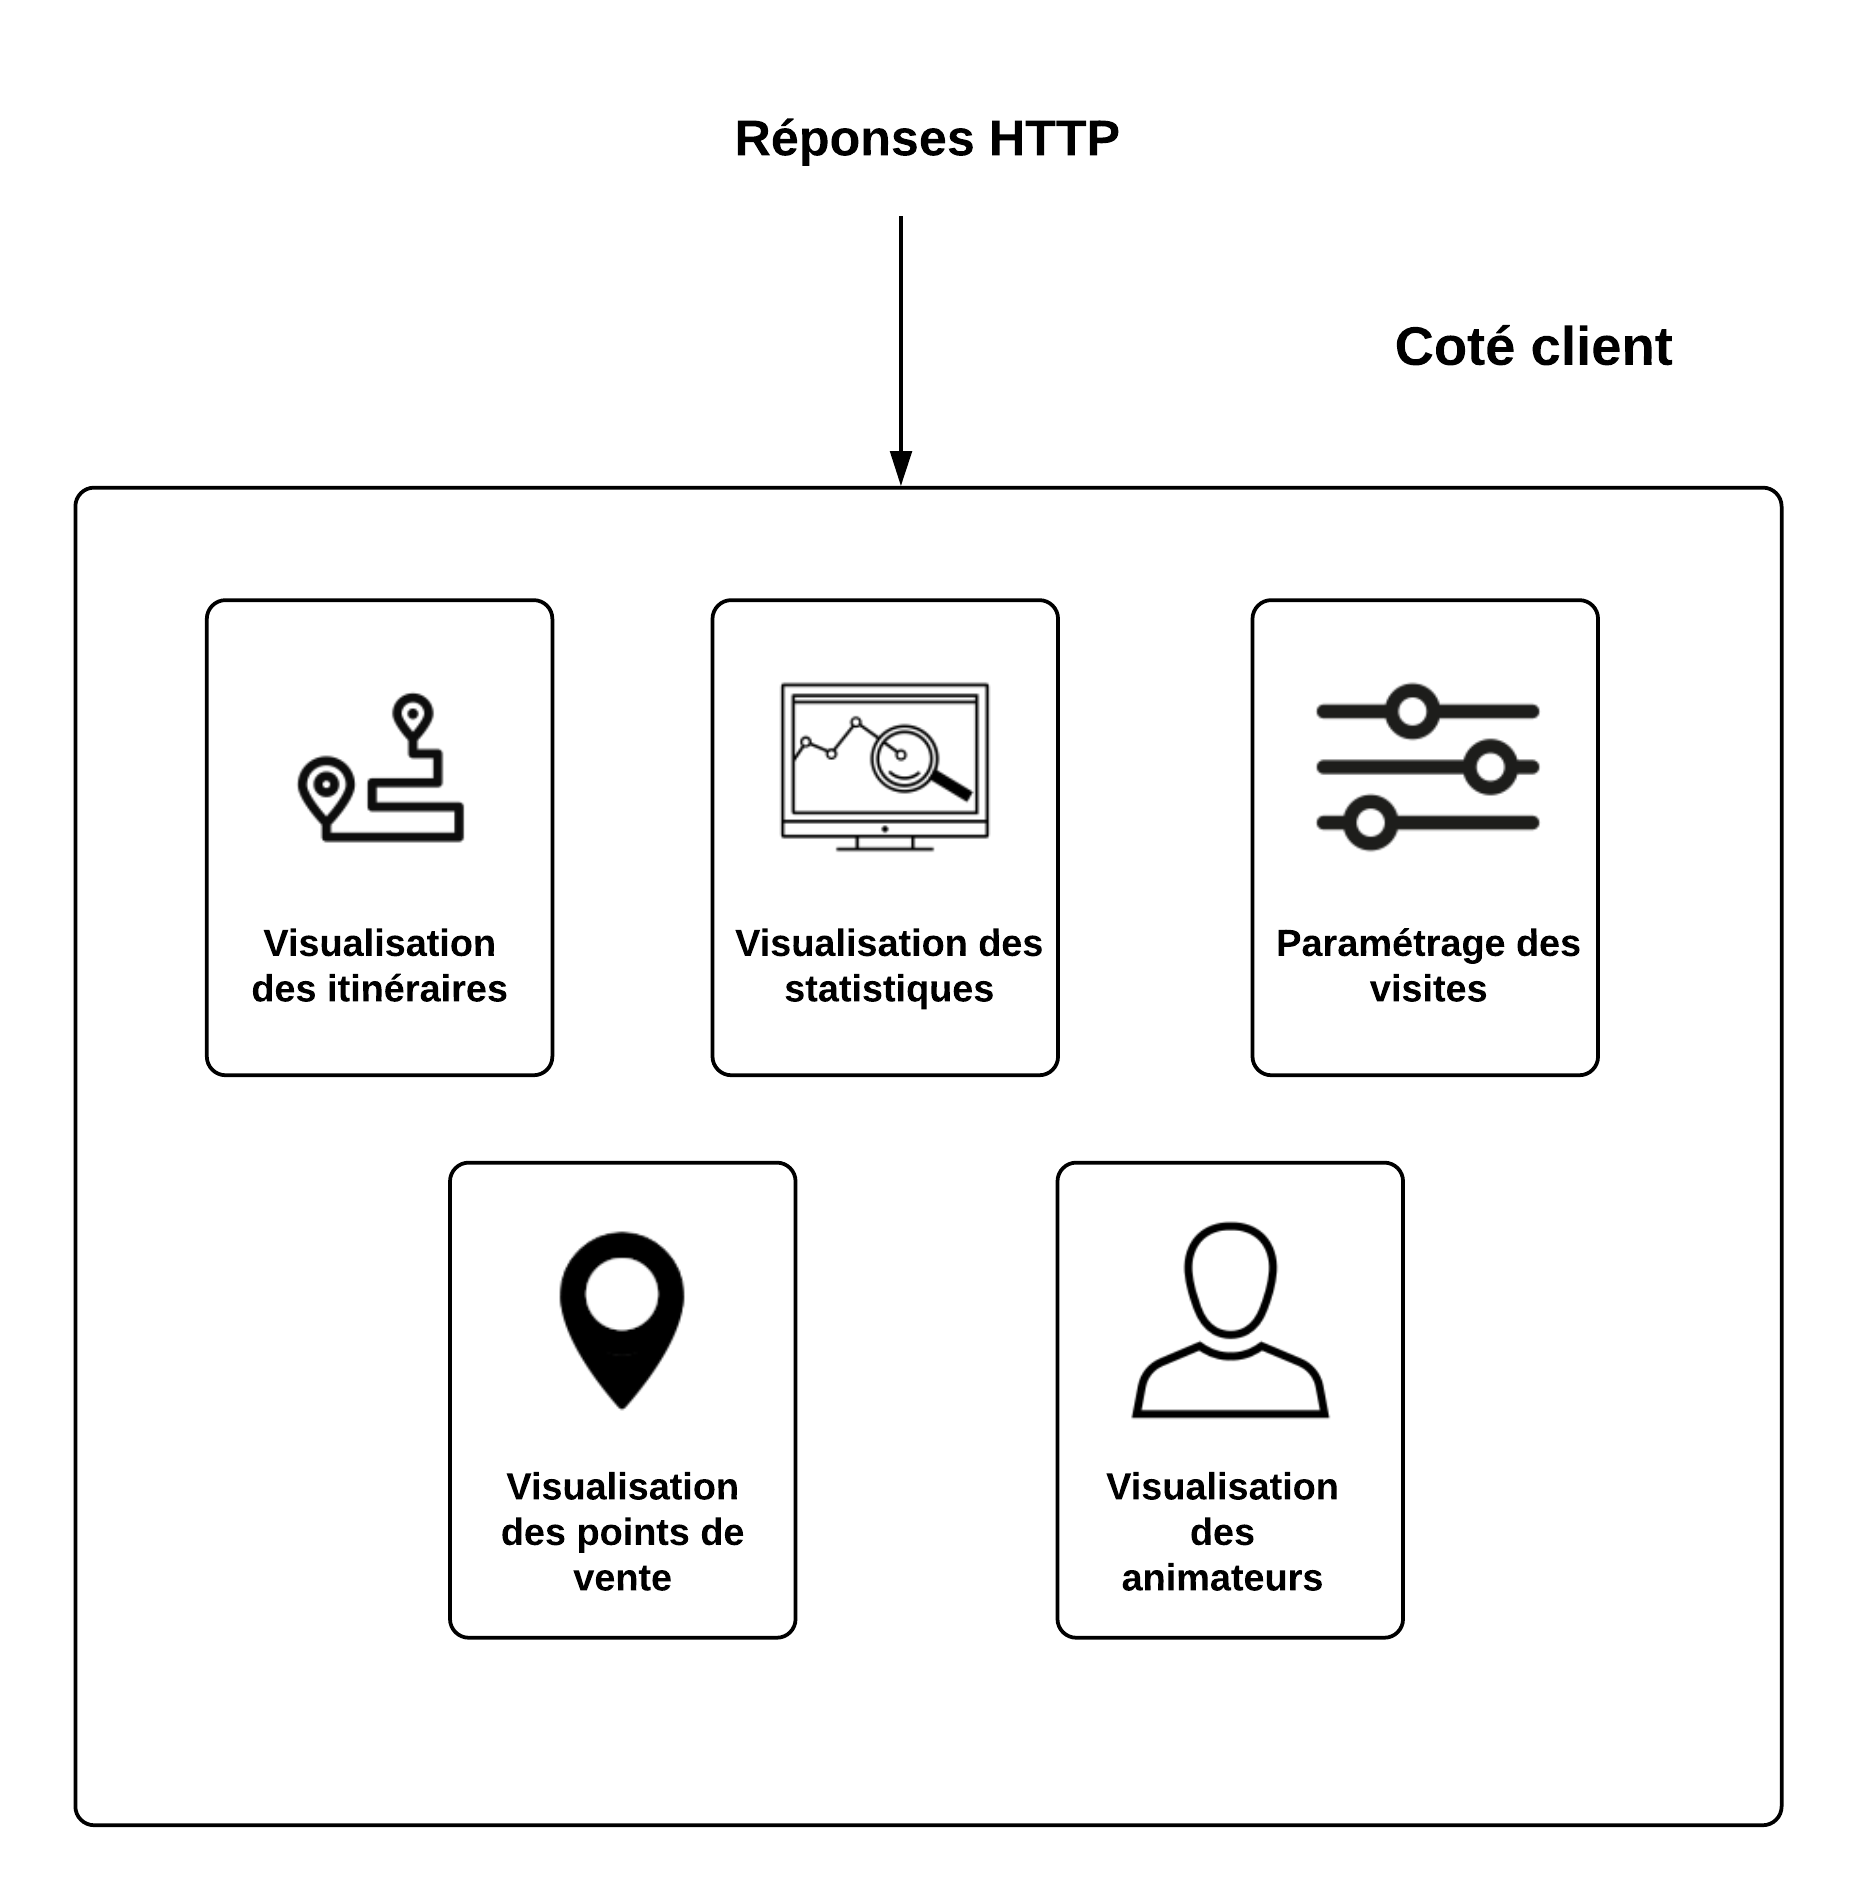
\includegraphics[height=10cm]{images_pfe/CLIENT_SIDE.png}
  \caption{Partie client.}
  \label{fig:client-side}
\end{figure}
\FloatBarrier



\section{Conclusion}
Lorem ipsum dolor sit amet, consectetur adipiscing elit. Proin posuere euismod neque, non semper nibh viverra sed. Praesent ut varius magna. Fusce ipsum ante, semper nec interdum at, semper et lacus. Nulla ultrices magna a fringilla finibus. Etiam sollicitudin blandit ante. Vivamus blandit rhoncus tincidunt. Morbi sit amet congue purus. Praesent interdum gravida congue. Donec fermentum dui fermentum maximus rutrum.

Lorem ipsum dolor sit amet, consectetur adipiscing elit. Proin posuere euismod neque, non semper nibh viverra sed. Praesent ut varius magna. Fusce ipsum ante, semper nec interdum at, semper et lacus. Nulla ultrices magna a fringilla finibus. Etiam sollicitudin blandit ante. Vivamus blandit rhoncus tincidunt. Morbi sit amet congue purus. Praesent interdum gravida congue. Donec fermentum dui fermentum maximus rutrum.

Lorem ipsum dolor sit amet, consectetur adipiscing elit. Proin posuere euismod neque, non semper nibh viverra sed. Praesent ut varius magna. Fusce ipsum ante, semper nec interdum at, semper et lacus. Nulla ultrices magna a fringilla finibus. Etiam sollicitudin blandit ante. Vivamus blandit rhoncus tincidunt. Morbi sit amet congue purus. Praesent interdum gravida congue. Donec fermentum dui fermentum maximus rutrum.


\chapter{Réalisation}

\newpage

\section{Introduction}
Lorem ipsum dolor sit amet, consectetur adipiscing elit. Proin posuere euismod neque, non semper nibh viverra sed. Praesent ut varius magna. Fusce ipsum ante, semper nec interdum at, semper et lacus. Nulla ultrices magna a fringilla finibus. Etiam sollicitudin blandit ante. Vivamus blandit rhoncus tincidunt. Morbi sit amet congue purus. Praesent interdum gravida congue. Donec fermentum dui fermentum maximus rutrum.

\section{Architecture technique de la solution}

\begin{figure}[hbt!]
  \centering
  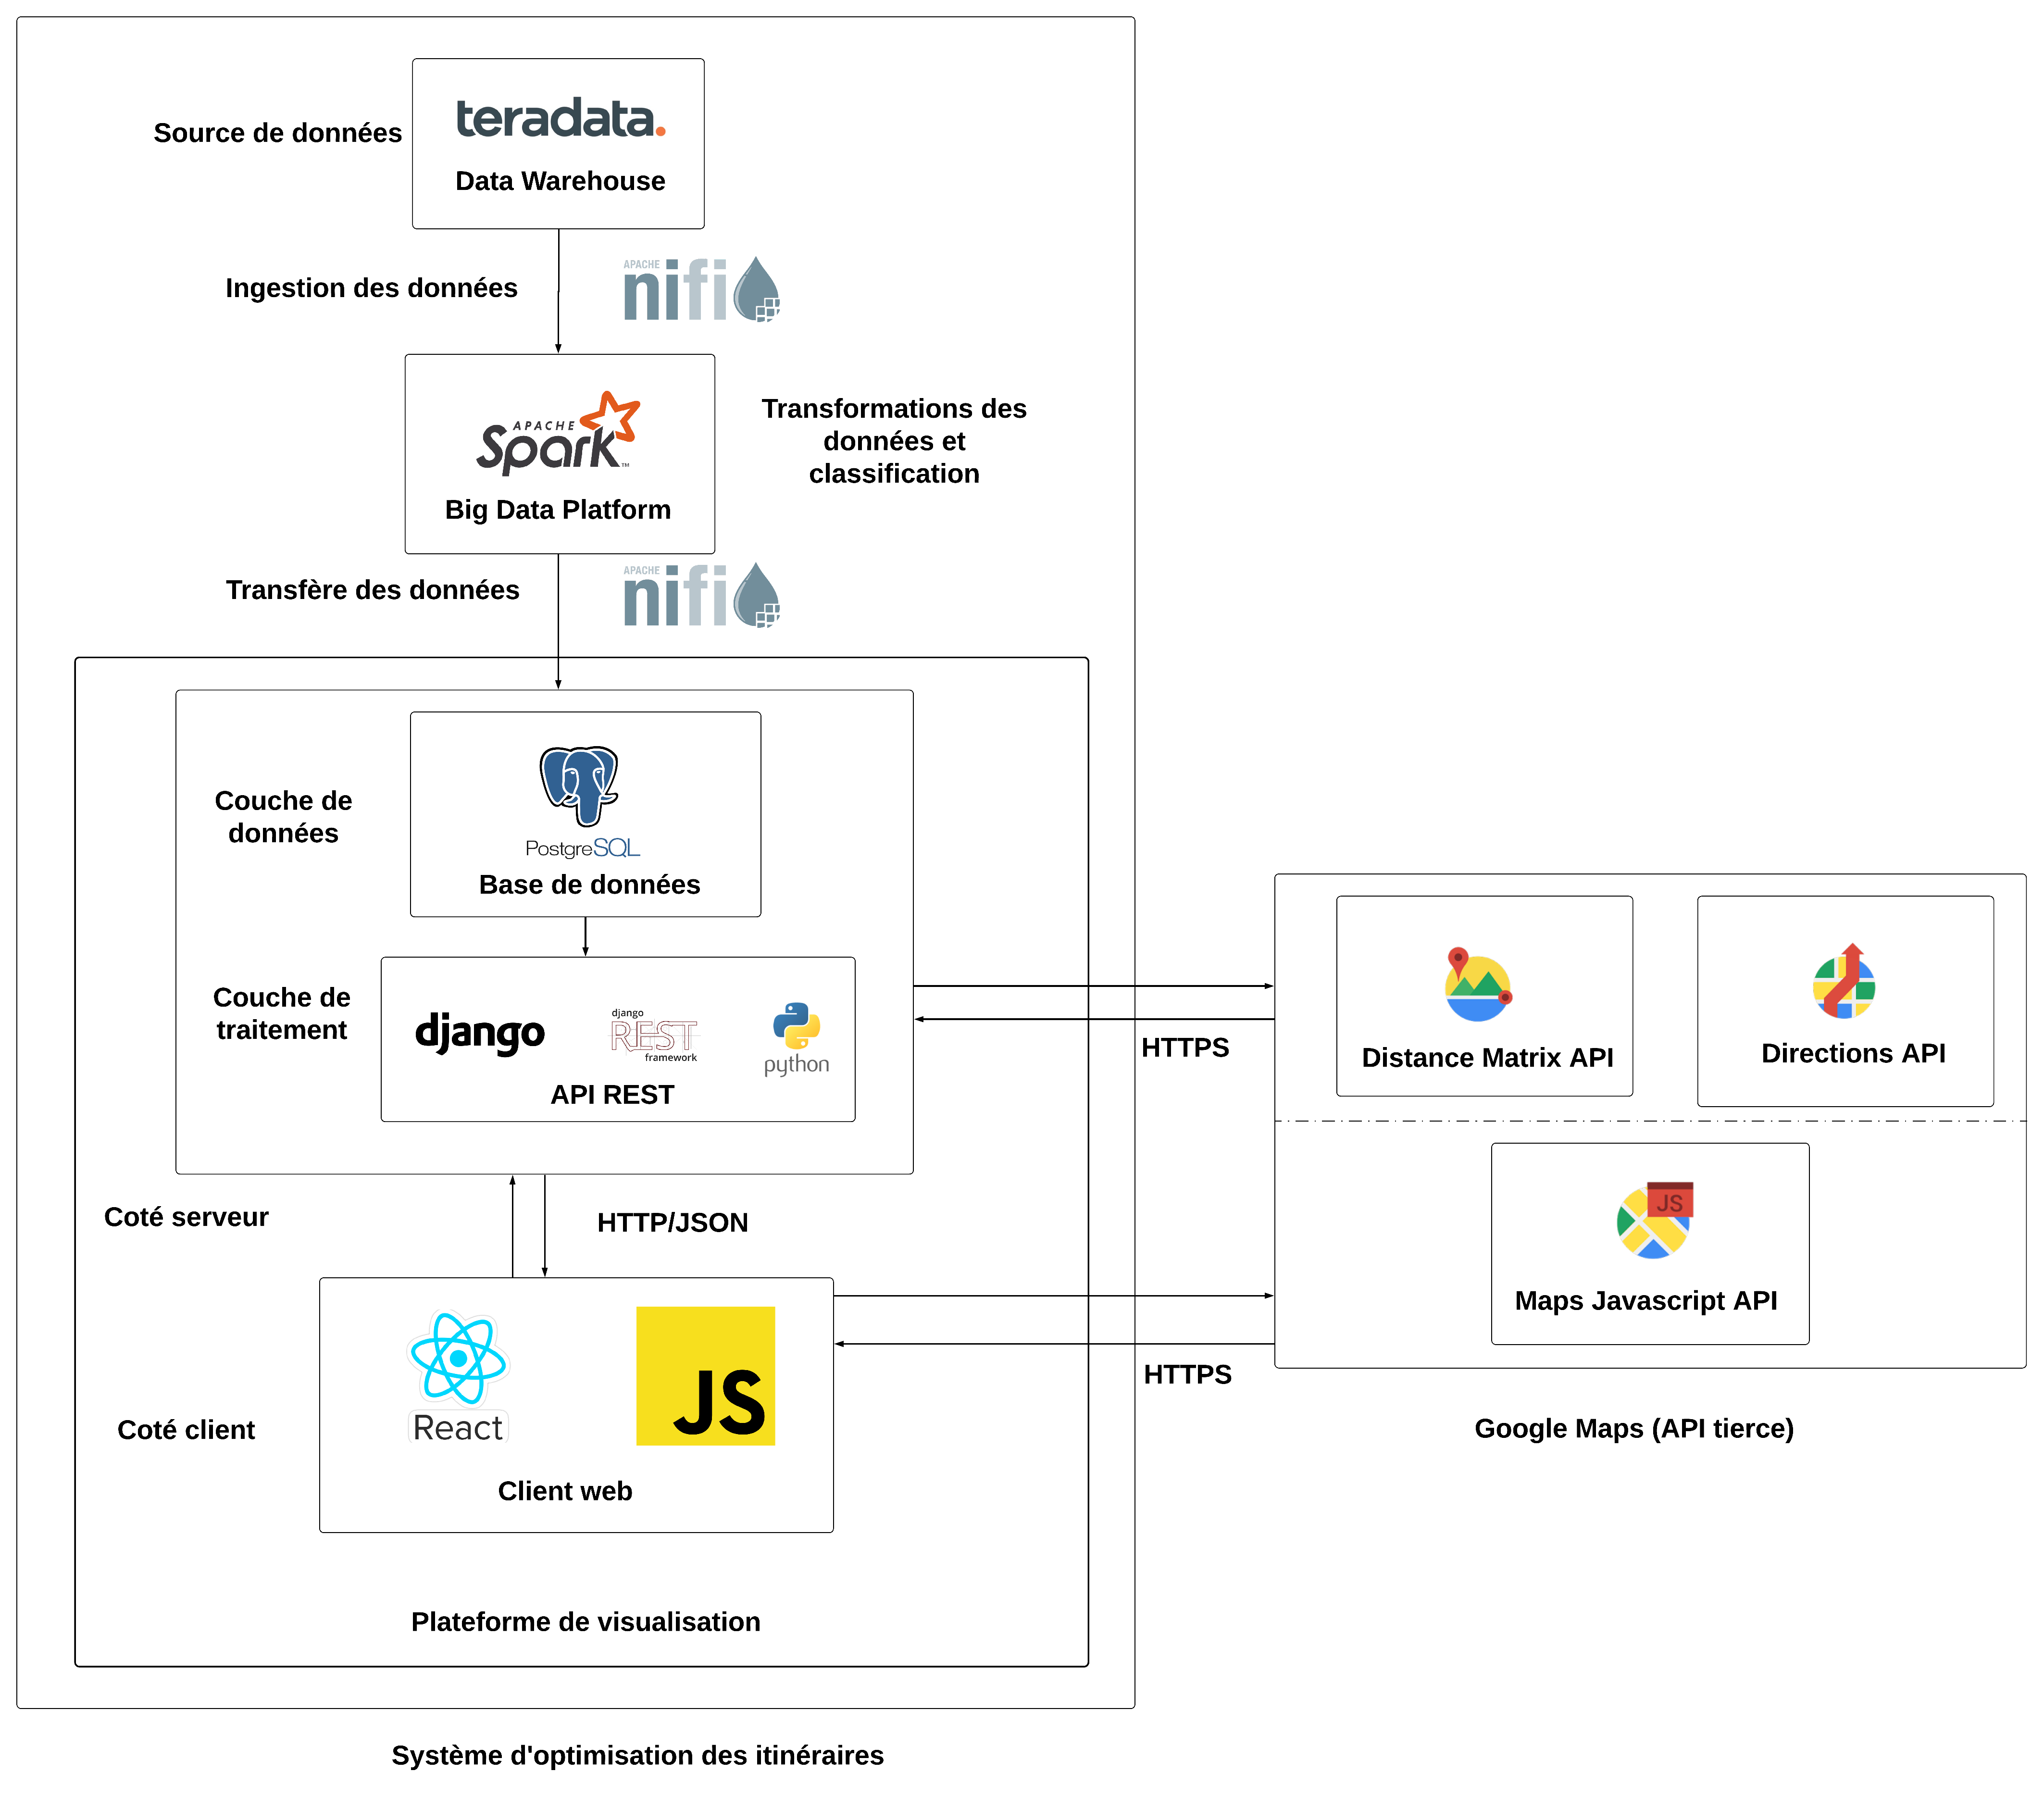
\includegraphics[height=15cm]{images_pfe/SYSTEM_ARCHITECTURE.png}
  \caption{Architecture technique de la solution.}
  \label{fig:technical-architecture}
\end{figure}
\FloatBarrier

La figure \ref{fig:technical-architecture} Lorem ipsum dolor sit amet, consectetur adipiscing elit. Proin posuere euismod neque, non semper nibh viverra sed. Praesent ut varius magna.Lorem ipsum dolor sit amet, consectetur adipiscing elit. Proin posuere euismod neque, non semper nibh viverra sed. Praesent ut varius magna. \textbf{Teradata Database} et il Lorem ipsum dolor sit amet, consectetur adipiscing elit. Proin posuere euismod neque, non semper nibh viverra sed. Praesent ut varius magna. \textbf{Apache Nifi} Lorem ipsum dolor sit amet, consectetur adipiscing elit. Proin posuere euismod neque, non semper nibh viverra sed. Praesent ut varius magna. \textbf{Apache Spark} via l'API Python \textbf{PySpark}. Lorem ipsum dolor sit amet, consectetur adipiscing elit. Proin posuere euismod neque, non semper nibh viverra sed. Praesent ut varius magna. \textbf{PostgreSQL} Lorem ipsum dolor sit amet, consectetur adipiscing elit. Proin posuere euismod neque, non semper nibh viverra sed. Praesent ut varius magna. \textbf{Django} sous le langage \textbf{Python}. Lorem ipsum dolor sit amet, consectetur adipiscing elit. Proin posuere euismod neque, non semper nibh viverra sed. Praesent ut varius magna. \textbf{Django Rest}. Le client web quant à lui, est implémenté avec la librairie \textbf{React.js} sous le langage \textbf{Javascript}. Le système communique avec les APIs \textbf{Google Maps} Lorem ipsum dolor sit amet, consectetur adipiscing elit. Proin posuere euismod neque, non semper nibh viverra sed. Praesent ut varius magna.I \textbf{Distance Matrix} Lorem ipsum dolor sit amet, consectetur adipiscing elit. Proin posuere euismod neque, non semper nibh viverra sed. Praesent ut varius magna. \textbf{Directions} Lorem ipsum dolor sit amet, consectetur adipiscing elit. Proin posuere euismod neque, non semper nibh viverra sed. Praesent ut varius magna.\textbf{Maps} Lorem ipsum dolor sit amet, consectetur adipiscing elit. Proin posuere euismod neque, non semper nibh viverra sed. Praesent ut varius magna.

\section{Technologies utilisées}

\subsection*{Teradata Database}

\begin{wrapfigure}{r}{0.3\textwidth}
  \centering
  
\includegraphics[width=0.28\textwidth]{images_pfe/Teradata_logo_2018.png}
  \caption{Logo de Teradata.}
\end{wrapfigure}
\FloatBarrier
Teradata Database \footnote{\url{https://www.teradata.com/} (visité le 11/08/2020).} Lorem ipsum dolor sit amet, consectetur adipiscing elit. Proin posuere euismod neque, non semper nibh viverra sed. Praesent ut varius magna. Fusce ipsum ante, semper nec interdum at, semper et lacus. Nulla ultrices magna a fringilla finibus. Etiam sollicitudin blandit ante. Vivamus blandit rhoncus tincidunt. Morbi sit amet congue purus. Praesent interdum gravida congue. Donec fermentum dui fermentum maximus rutrum.

\subsection*{Apache Nifi}
\begin{wrapfigure}{r}{0.3\textwidth}
  \centering
  
\includegraphics[width=0.2\textwidth]{images_pfe/apache_nifi_logo.png}
  \caption{Logo de Nifi.}
\end{wrapfigure}
\FloatBarrier
Apache Nifi \footnote{\url{https://nifi.apache.org/} (visité le 11/08/2020).} Lorem ipsum dolor sit amet, consectetur adipiscing elit. Proin posuere euismod neque, non semper nibh viverra sed. Praesent ut varius magna. Fusce ipsum ante, semper nec interdum at, semper et lacus. Nulla ultrices magna a fringilla finibus. Etiam sollicitudin blandit ante. Vivamus blandit rhoncus tincidunt. Morbi sit amet congue purus. Praesent interdum gravida congue. Donec fermentum dui fermentum maximus rutrum.


\subsection*{Apache Spark}
\begin{wrapfigure}{r}{0.3\textwidth}
  \centering
  
\includegraphics[width=0.28\textwidth]{images_pfe/Apache_Spark_logo.png}
  \caption{Logo de Spark.}
\end{wrapfigure}
\FloatBarrier
Apache Spark \footnote{\url{https://spark.apache.org/} (visité le 11/08/2020).} Lorem ipsum dolor sit amet, consectetur adipiscing elit. Proin posuere euismod neque, non semper nibh viverra sed. Praesent ut varius magna. (\textbf{PySpark}) Lorem ipsum dolor sit amet, consectetur adipiscing elit. Proin posuere euismod neque, non semper nibh viverra sed. Praesent ut varius magna. Fusce ipsum ante, semper nec interdum at, semper et lacus. Nulla ultrices magna a fringilla finibus. Etiam sollicitudin blandit ante. Vivamus blandit rhoncus tincidunt. Morbi sit amet congue purus. Praesent interdum gravida congue. Donec fermentum dui fermentum maximus rutrum.


\subsection*{PostgreSQL}
\begin{wrapfigure}[9]{r}{0.3\textwidth}
  \centering
  
\includegraphics[width=0.2\textwidth]{images_pfe/postgres_logo.png}
  \caption{Logo de PostgreSQL.}
\end{wrapfigure}
\FloatBarrier
PostgreSQL \footnote{\url{https://www.postgresql.org/} (visité le 11/08/2020).} Lorem ipsum dolor sit amet, consectetur adipiscing elit. Proin posuere euismod neque, non semper nibh viverra sed. Praesent ut varius magna. Fusce ipsum ante, semper nec interdum at, semper et lacus. Nulla ultrices magna a fringilla finibus. Etiam sollicitudin blandit ante. Vivamus blandit rhoncus tincidunt. Morbi sit amet congue purus. Praesent interdum gravida congue. Donec fermentum dui fermentum maximus rutrum.


\subsection*{Python}

\begin{wrapfigure}[6]{r}{0.3\textwidth}
  \centering
  
\includegraphics[width=0.12\textwidth]{images_pfe/python_logo.png}
  \caption{Logo de Python.}
\end{wrapfigure}
\FloatBarrier
Python \footnote{\url{https://www.python.org/} (visité le 11/08/2020).} Lorem ipsum dolor sit amet, consectetur adipiscing elit. Proin posuere euismod neque, non semper nibh viverra sed. Praesent ut varius magna. Fusce ipsum ante, semper nec interdum at, semper et lacus. Nulla ultrices magna a fringilla finibus. Etiam sollicitudin blandit ante. Vivamus blandit rhoncus tincidunt. Morbi sit amet congue purus.

\vspace{.5cm}

\subsection*{Django}

\begin{wrapfigure}{r}{0.3\textwidth}
  \centering
  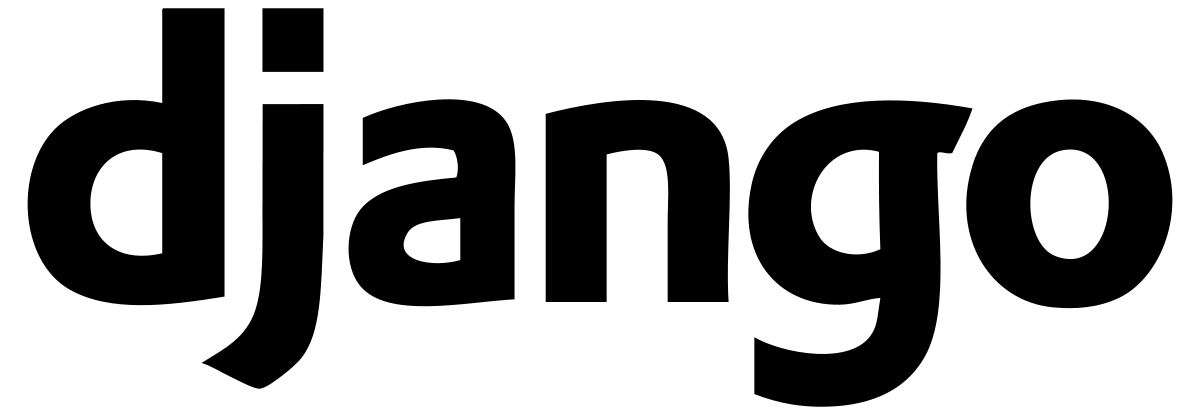
\includegraphics[width=0.2\textwidth]{images_pfe/django_logo.png}
  \caption{Logo de Django.}
\end{wrapfigure}
\FloatBarrier
Django \footnote{\url{https://www.djangoproject.com/} (visité le 11/08/2020).} Lorem ipsum dolor sit amet, consectetur adipiscing elit. Proin posuere euismod neque, non semper nibh viverra sed. Praesent ut varius magna. Fusce ipsum ante, semper nec interdum at, semper et lacus. Nulla ultrices magna a fringilla finibus. Etiam sollicitudin blandit ante. Vivamus blandit rhoncus tincidunt. Morbi sit amet congue purus. Praesent interdum gravida congue. Donec fermentum dui fermentum maximus rutrum.

\vspace{.5cm}

\subsection*{Django Rest Framework}

\begin{wrapfigure}{r}{0.3\textwidth}
  \centering
  
\includegraphics[width=0.25\textwidth]{images_pfe/django_rest.png}
  \caption{Logo de Django Rest Framework.}
\end{wrapfigure}
\FloatBarrier
Django REST \footnote{\url{https://www.django-rest-framework.org/} (visité le 11/08/2020).}Lorem ipsum dolor sit amet, consectetur adipiscing elit. Proin posuere euismod neque, non semper nibh viverra sed. Praesent ut varius magna. Fusce ipsum ante, semper nec interdum at, semper et lacus. Nulla ultrices magna a fringilla finibus. Etiam sollicitudin blandit ante. Vivamus blandit rhoncus tincidunt. Morbi sit amet congue purus. Praesent interdum gravida congue. Donec fermentum dui fermentum maximus rutrum.

\vspace{.5cm}

\subsection*{Javascript}
\begin{wrapfigure}[6]{r}{0.3\textwidth}
  \centering
  
\includegraphics[width=0.2\textwidth]{images_pfe/js_logo.png}
  \caption{Logo de Javascript.}
\end{wrapfigure}
\FloatBarrier
JavaScript \footnote{\url{https://developer.mozilla.org/fr/docs/Web/JavaScript} (visité le 11/08/2020).} Lorem ipsum dolor sit amet, consectetur adipiscing elit. Proin posuere euismod neque, non semper nibh viverra sed. Praesent ut varius magna. Fusce ipsum ante, semper nec interdum at, semper et lacus. Nulla ultrices magna a fringilla finibus. Etiam sollicitudin blandit ante. Vivamus blandit rhoncus tincidunt. Morbi sit amet congue purus. Praesent interdum gravida congue. 

\vspace{3cm}

\subsection*{React.js}

\begin{wrapfigure}[6]{r}{0.3\textwidth}
  \centering
  
\includegraphics[width=0.2\textwidth]{images_pfe/react_logo.png}
  \caption{Logo de React.js.}
\end{wrapfigure}
\FloatBarrier
React.js \footnote{\url{https://fr.reactjs.org/} (visité le 12/08/2020).} Lorem ipsum dolor sit amet, consectetur adipiscing elit. Proin posuere euismod neque, non semper nibh viverra sed. Praesent ut varius magna. Fusce ipsum ante, semper nec interdum at, semper et lacus. Nulla ultrices magna a fringilla finibus. Etiam sollicitudin blandit ante. Vivamus blandit rhoncus tincidunt. Morbi sit amet congue purus. 

\vspace{1cm}

\subsection*{Distance Matrix API}
\begin{wrapfigure}[6]{r}{0.3\textwidth}
  \centering
  
\includegraphics[width=0.2\textwidth]{images_pfe/google_distance_matrix_api.png}
  \caption{Logo de l'API Distance Matrix.}
\end{wrapfigure}
\FloatBarrier
L'API Distance Matrix \footnote{\url{https://developers.google.com/maps/documentation/distance-matrix/overview} (visité le 12/08/2020).} Lorem ipsum dolor sit amet, consectetur adipiscing elit. Proin posuere euismod neque, non semper nibh viverra sed. Praesent ut varius magna. Fusce ipsum ante, semper nec interdum at, semper et lacus. Nulla ultrices magna a fringilla finibus. Etiam sollicitudin blandit ante. Vivamus blandit rhoncus tincidunt. Morbi sit amet congue purus. 

\vspace{1cm}

\subsection*{Directions API}
\begin{wrapfigure}[6]{r}{0.3\textwidth}
  \centering
  
\includegraphics[width=0.2\textwidth]{images_pfe/google_directions_api.png}
  \caption{Logo de l'API Directions.}
\end{wrapfigure}
\FloatBarrier
L'API Directions \footnote{\url{https://developers.google.com/maps/documentation/directions/overview} (visité le 12/08/2020).} Lorem ipsum dolor sit amet, consectetur adipiscing elit. Proin posuere euismod neque, non semper nibh viverra sed. Praesent ut varius magna. Fusce ipsum ante, semper nec interdum at, semper et lacus. Nulla ultrices magna a fringilla finibus. Etiam sollicitudin blandit ante. Vivamus blandit rhoncus tincidunt. Morbi sit amet congue purus. 

\vspace{1cm}

\subsection*{Maps Javascript API}
\begin{wrapfigure}[6]{r}{0.3\textwidth}
  \centering
  
\includegraphics[width=0.2\textwidth]{images_pfe/google_maps_js.png}
  \caption{Logo de l'API Maps Javascript.}
\end{wrapfigure}
\FloatBarrier
L'API Maps JavaScript \footnote{\url{https://developers.google.com/maps/documentation/javascript/overview} (visité le 12/08/2020).} Lorem ipsum dolor sit amet, consectetur adipiscing elit. Proin posuere euismod neque, non semper nibh viverra sed. Praesent ut varius magna. Fusce ipsum ante, semper nec interdum at, semper et lacus. Nulla ultrices magna a fringilla finibus. Etiam sollicitudin blandit ante. Vivamus blandit rhoncus tincidunt. Morbi sit amet congue purus. Praesent interdum gravida congue. 

\vspace{1cm}

\section{Conclusion}
Lorem ipsum dolor sit amet, consectetur adipiscing elit. Proin posuere euismod neque, non semper nibh viverra sed. Praesent ut varius magna. Fusce ipsum ante, semper nec interdum at, semper et lacus. Nulla ultrices magna a fringilla finibus. Etiam sollicitudin blandit ante. Vivamus blandit rhoncus tincidunt. Morbi sit amet congue purus. Praesent interdum gravida congue. Donec fermentum dui fermentum maximus rutrum.














\chapter{Tests et résultats}
\clearpage
\section{Introduction}
Lorem ipsum dolor sit amet, consectetur adipiscing elit. Proin posuere euismod neque, non semper nibh viverra sed. Praesent ut varius magna. Fusce ipsum ante, semper nec interdum at, semper et lacus. Nulla ultrices magna a fringilla finibus. Etiam sollicitudin blandit ante. Vivamus blandit rhoncus tincidunt. Morbi sit amet congue purus. Praesent interdum gravida congue. Donec fermentum dui fermentum maximus rutrum.


\subsection{Analyse des variables}
L'objectif de l'analyse des variables (Voir annexe \ref{app:initial-dataset}) était d'identifier les relations et les corrélations contenues dans les données. Pour cela nous avons utilisé deux méthodes : la matrice de corrélation (Voir figure \ref{fig:all-features-correlations}) et la matrice de puissance prédictive (Voir figure \ref{fig:all-features-pps}). La matrice de corrélation contient les coefficients de corrélation entre chaque paire de variable (Voir annexe \ref{app:correlation}). 

\begin{figure}[hbt!]
  \centering
  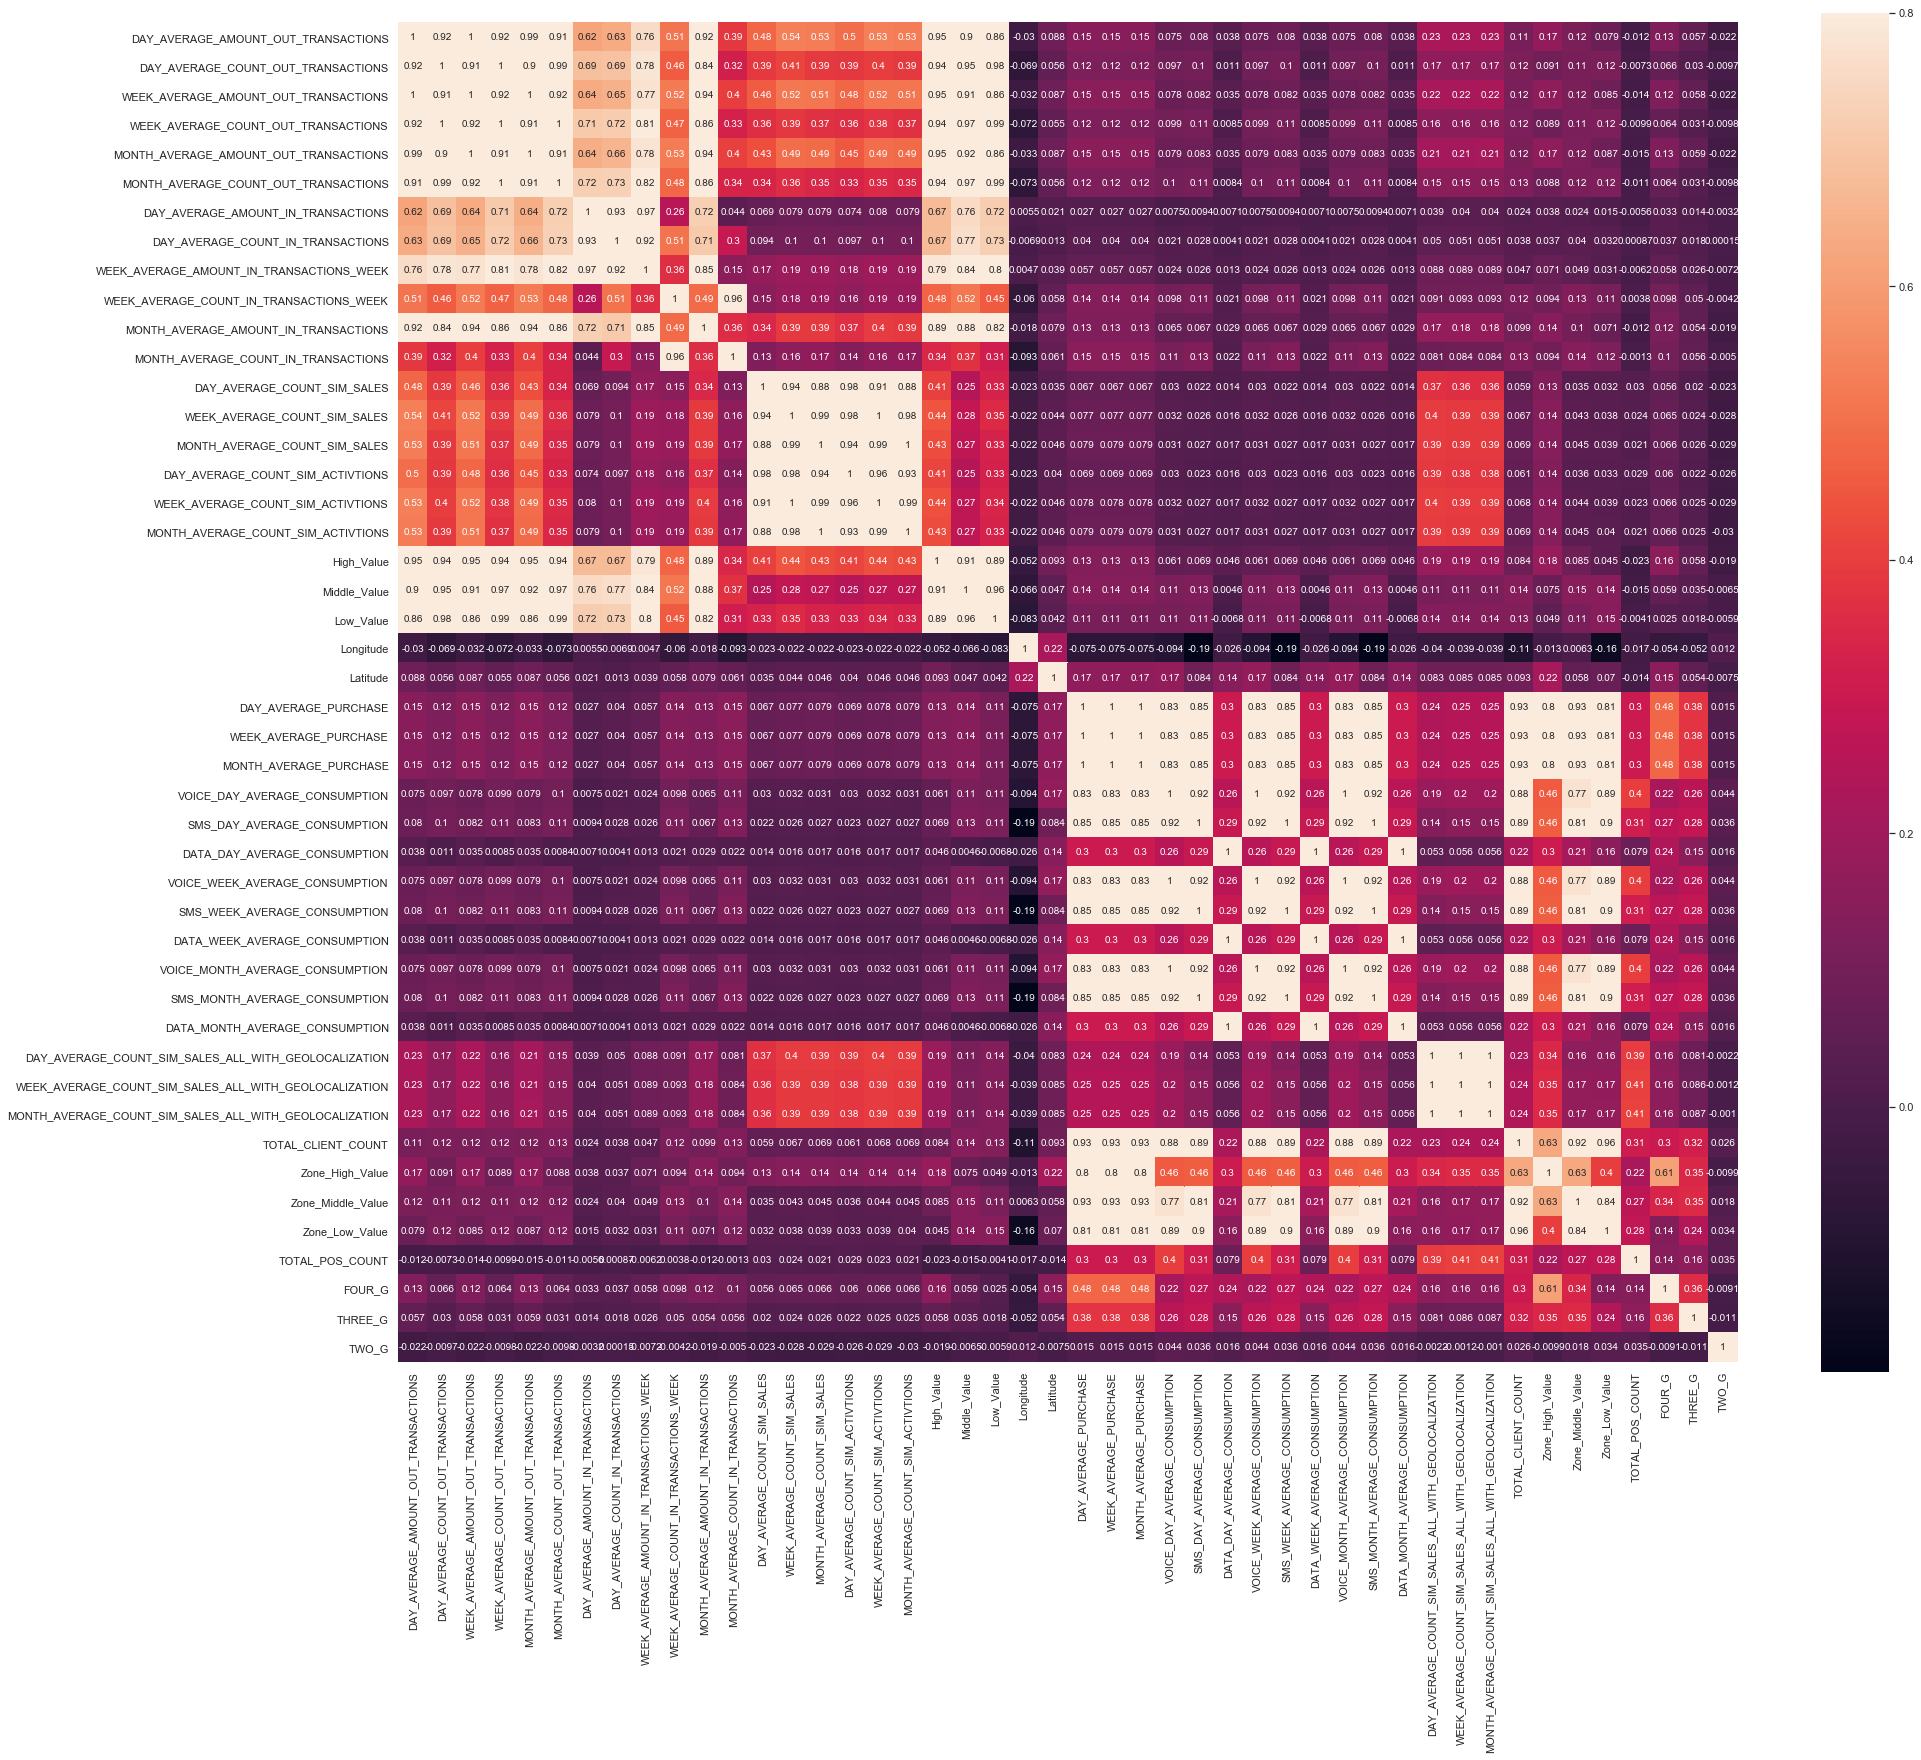
\includegraphics[width=12cm]{images_pfe/features_correlations.png}
  \caption{Matrice de corrélation (les couleurs claires désignent une forte corrélation).}
  \label{fig:all-features-correlations}
\end{figure}
\FloatBarrier

Lorem ipsum dolor sit amet, consectetur adipiscing elit. Proin posuere euismod neque, non semper nibh viverra sed. Praesent ut varius magna. Fusce ipsum ante, semper nec interdum at, semper et lacus. Nulla ultrices magna a fringilla finibus. Etiam sollicitudin blandit ante. Vivamus blandit rhoncus tincidunt. Morbi sit amet congue purus. Praesent interdum gravida congue. Donec fermentum dui fermentum maximus rutrum. Le score de puissance de prédiction entre une variable $X$ et une variable $Y$ représente la précision avec validation croisée du modèle contenant la variable $X$ seulement pour prédire la variable $Y$. Lorem ipsum dolor sit amet, consectetur adipiscing elit. Proin posuere euismod neque, non semper nibh viverra sed. Praesent ut varius magna. Fusce ipsum ante, semper nec interdum at, semper et lacus. Nulla ultrices magna a fringilla finibus. Etiam sollicitudin blandit ante. Vivamus blandit rhoncus tincidunt. Morbi sit amet congue purus. Praesent interdum gravida congue. Donec fermentum dui fermentum maximus rutrum. \parencite{wetschoreck_rip_2020}.

\begin{figure}[hbt!]
  \centering
  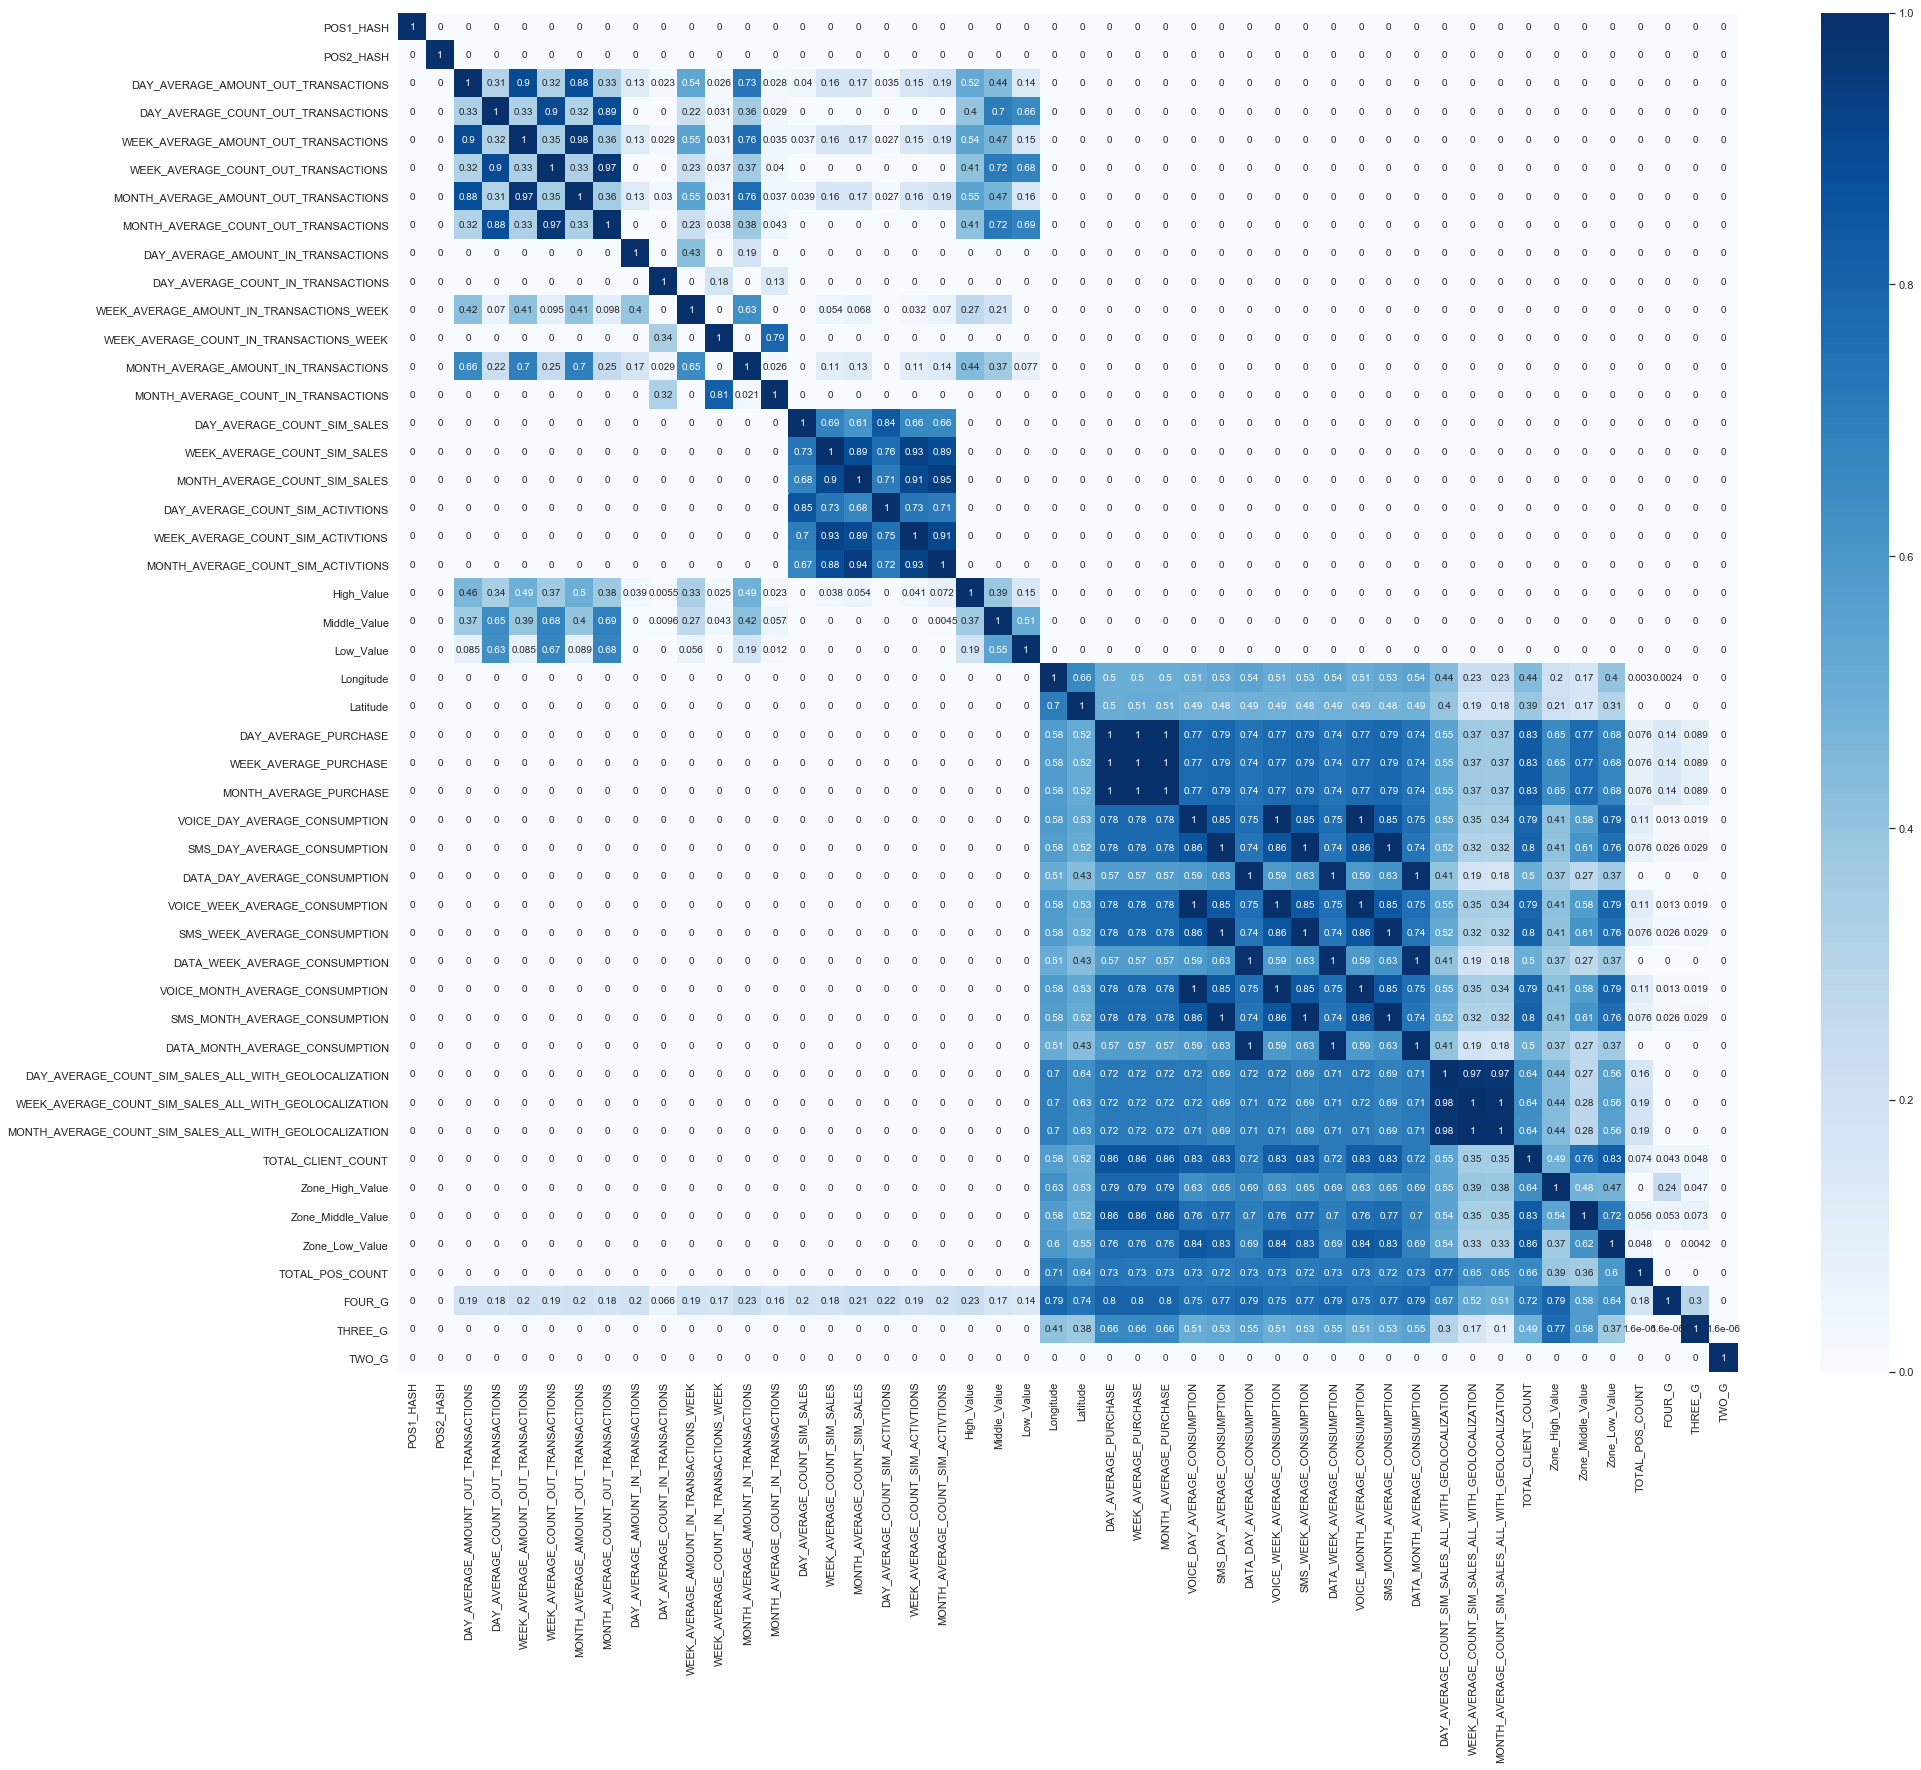
\includegraphics[width=12cm]{images_pfe/features_pps.png}
  \caption{Matrice de puissance de prédiction (les couleurs foncées désignent une forte puissance de prédiction).}
  \label{fig:all-features-pps}
\end{figure}
\FloatBarrier

La première remarque que nous tirons de la matrice de corrélation (figure \ref{fig:all-features-correlations}) Lorem ipsum dolor sit amet, consectetur adipiscing elit. Proin posuere euismod neque, non semper nibh viverra sed. Praesent ut varius magna. Fusce ipsum ante, semper nec interdum at, semper et lacus. Nulla ultrices magna a fringilla finibus. Etiam sollicitudin blandit ante. Vivamus blandit rhoncus tincidunt. Morbi sit amet congue purus. Praesent interdum gravida congue. Donec fermentum dui fermentum maximus rutrum. (Voir annexe \ref{app:initial-dataset}).Lorem ipsum dolor sit amet, consectetur adipiscing elit. Proin posuere euismod neque, non semper nibh viverra sed. Praesent ut varius magna. Fusce ipsum ante, semper nec interdum at, semper et lacus. Nulla ultrices magna a fringilla finibus. Etiam sollicitudin blandit ante. Vivamus blandit rhoncus tincidunt. Morbi sit amet congue purus. Praesent interdum gravida congue. Donec fermentum dui fermentum maximus rutrum.

\medskip

Lorem ipsum dolor sit amet, consectetur adipiscing elit. Proin posuere euismod neque, non semper nibh viverra sed. Praesent ut varius magna. Fusce ipsum ante, semper nec interdum at, semper et lacus. Nulla ultrices magna a fringilla finibus. Etiam sollicitudin blandit ante. Vivamus blandit rhoncus tincidunt. Morbi sit amet congue purus. Praesent interdum gravida congue. Donec fermentum dui fermentum maximus rutrum.

\medskip

Les figures \ref{fig:chosen-features-correlations} Lorem ipsum dolor sit amet, consectetur adipiscing elit. Proin posuere euismod neque, non semper nibh viverra sed. Praesent ut varius magna. Fusce ipsum ante, semper nec interdum at, semper et lacus. Nulla ultrices magna a fringilla finibus. Etiam sollicitudin blandit ante. Vivamus blandit rhoncus tincidunt. Morbi sit amet congue purus. Praesent interdum gravida congue. Donec fermentum dui fermentum maximus rutrum. : \\

\begin{figure}[hbt!]
  \begin{subfigure}[t]{0.4\textwidth}
  \centering
  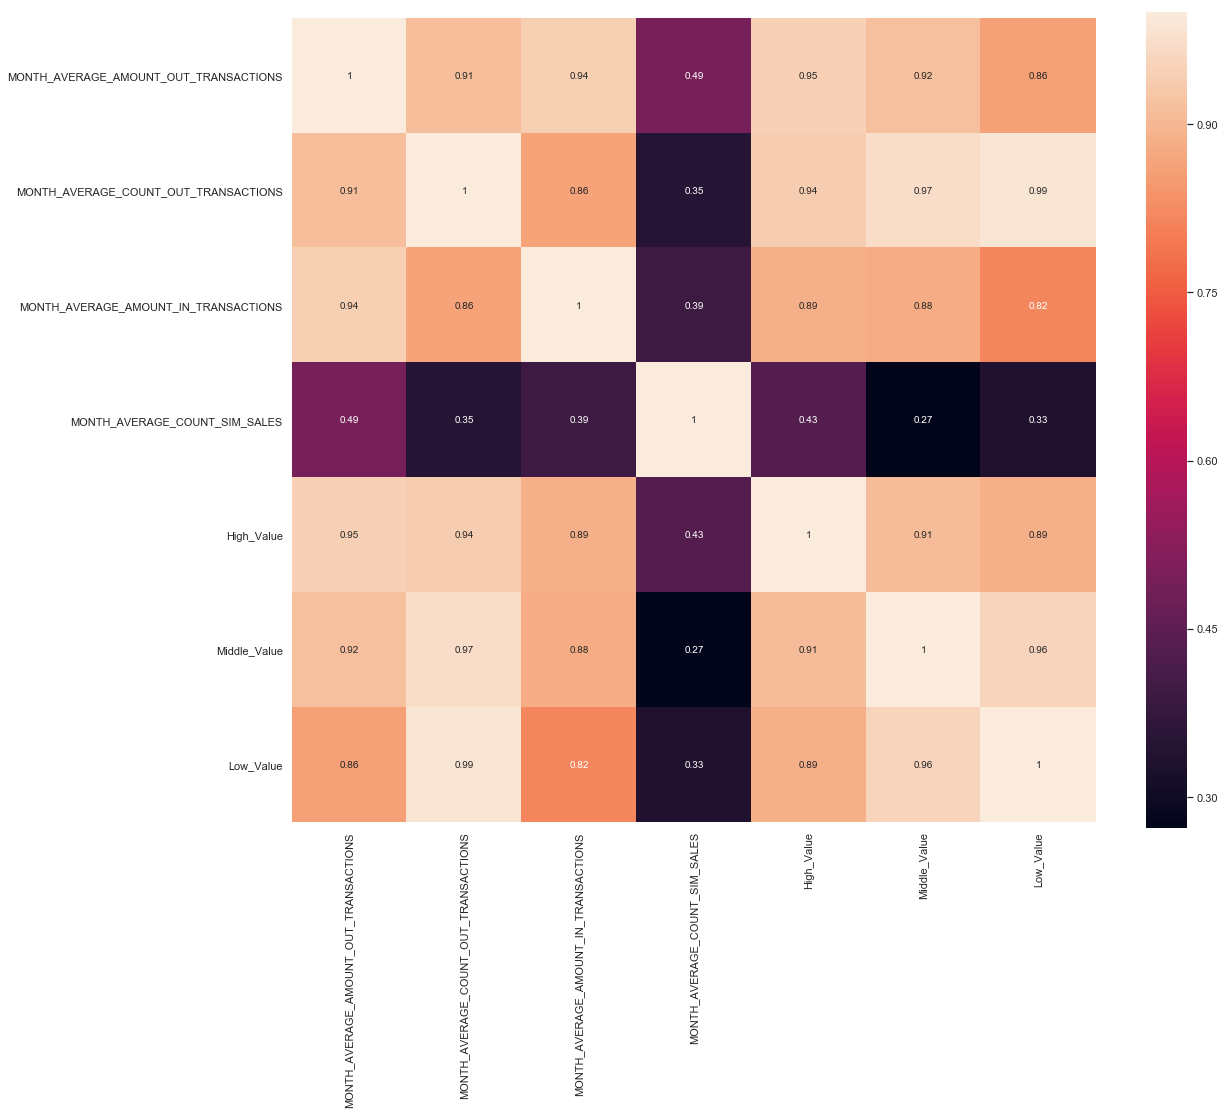
\includegraphics[width=\linewidth]{images_pfe/feature_correlations.png}
  \caption{Matrice de corrélation des variable sélectionnées.}
  \label{fig:chosen-features-correlations}
  \end{subfigure}\hfill
  \begin{subfigure}[t]{0.4\textwidth}
  \centering
  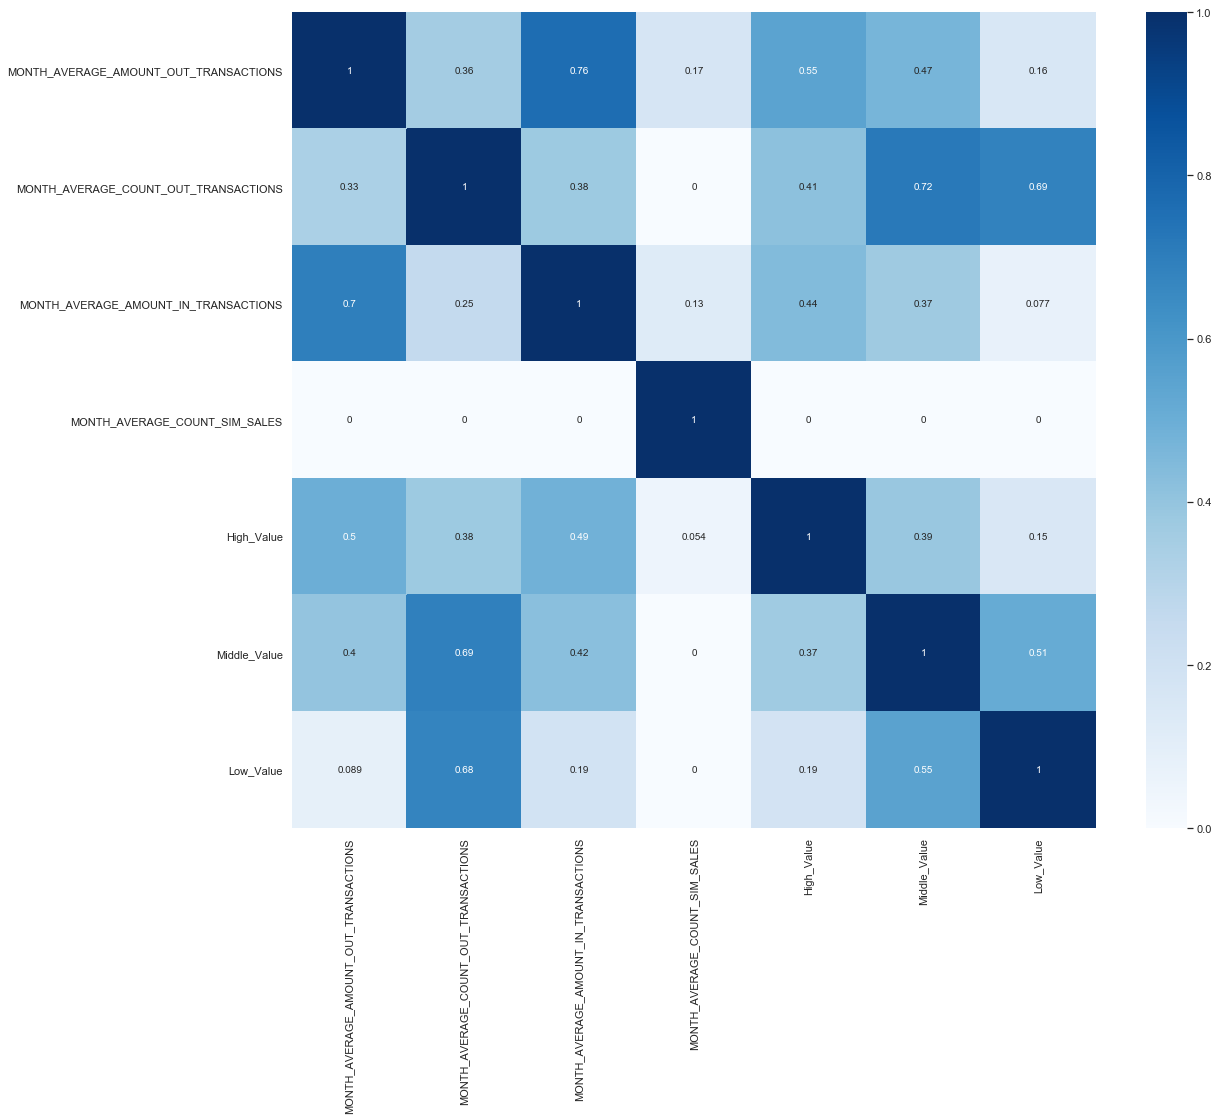
\includegraphics[width=\linewidth]{images_pfe/features_pps2.png}
  \caption{Matrice de puissance de prédiction des variables sélectionnées.}
  \label{fig:chosen-features-pps}
  \end{subfigure}
\end{figure}
\FloatBarrier


\subsection{Clustering}
Lorem ipsum dolor sit amet, consectetur adipiscing elit. Proin posuere euismod neque, non semper nibh viverra sed. Praesent ut varius magna. Fusce ipsum ante, semper nec interdum at, semper et lacus. Nulla ultrices magna a fringilla finibus. Etiam sollicitudin blandit ante. Vivamus blandit rhoncus tincidunt. Morbi sit amet congue purus. Praesent interdum gravida congue. Donec fermentum dui fermentum maximus rutrum.

\medskip

La première méthode était le clustering hiérarchique (Voir annexe \ref{app:hierarchical-clustering}). Lorem ipsum dolor sit amet, consectetur adipiscing elit. Proin posuere euismod neque, non semper nibh viverra sed. Praesent ut varius magna. Fusce ipsum ante, semper nec interdum at, semper et lacus. Nulla ultrices magna a fringilla finibus. Etiam sollicitudin blandit ante. Vivamus blandit rhoncus tincidunt. Morbi sit amet congue purus. Praesent interdum gravida congue. Donec fermentum dui fermentum maximus rutrum..

\begin{figure}[hbt!]
  \centering
  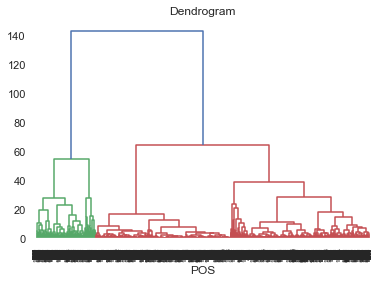
\includegraphics[width=10cm]{images_pfe/hirarchichal_clustering.png}
  \caption{Dendrogramme du clustering hiérarchique.}
  \label{fig:hierarchical-clustering}
\end{figure}
\FloatBarrier

La figure \ref{fig:hierarchical-clustering} Lorem ipsum dolor sit amet, consectetur adipiscing elit. Proin posuere euismod neque, non semper nibh viverra sed. Praesent ut varius magna. Fusce ipsum ante, semper nec interdum at, semper et lacus. Nulla ultrices magna a fringilla finibus. Etiam sollicitudin blandit ante. Vivamus blandit rhoncus tincidunt. Morbi sit amet congue purus. Praesent interdum gravida congue. Donec fermentum dui fermentum maximus rutrum. \ref{app:k-means}) Lorem ipsum dolor sit amet, consectetur adipiscing elit. Proin posuere euismod neque, non semper nibh viverra sed. Praesent ut varius magna. 

\medskip

Lorem ipsum dolor sit amet, consectetur adipiscing elit. Proin posuere euismod neque, non semper nibh viverra sed. Praesent ut varius magna. Fusce ipsum ante, semper nec interdum at, semper et lacus. Nulla ultrices magna a fringilla finibus. Etiam sollicitudin blandit ante. Vivamus blandit rhoncus tincidunt. Morbi sit amet congue purus. Praesent interdum gravida congue. Donec fermentum dui fermentum maximus rutrum. $K$ Lorem ipsum dolor sit amet, consectetur adipiscing elit. Proin posuere euismod neque, non semper nibh viverra sed. Praesent ut varius magna. Fusce ipsum ante, semper nec interdum at, semper et lacus. Nulla ultrices magna a fringilla finibus. Etiam sollicitudin blandit ante. Vivamus blandit rhoncus tincidunt. Morbi sit amet congue purus. Praesent interdum gravida congue. Donec fermentum dui fermentum maximus rutrum. \parencite{kassambara_determining_nodate}.

\begin{figure}[hbt!]
  \centering
  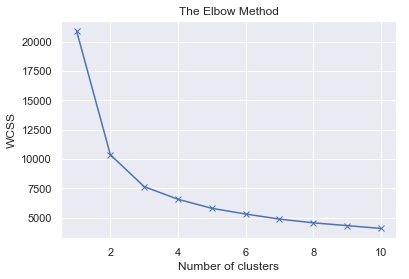
\includegraphics[width=10cm]{images_pfe/elbow_method.png}
  \caption{Résultat de la méthode Elbow.}
  \label{fig:elbow-method}
\end{figure}
\FloatBarrier

La figure \ref{fig:elbow-method}Lorem ipsum dolor sit amet, consectetur adipiscing elit. Proin posuere euismod neque, non semper nibh viverra sed. Praesent ut varius magna. Fusce ipsum ante, semper nec interdum at, semper et lacus. Nulla ultrices magna a fringilla finibus. Etiam sollicitudin blandit ante. Vivamus blandit rhoncus tincidunt. Morbi sit amet congue purus. Praesent interdum gravida congue. Donec fermentum dui fermentum maximus rutrum. $K$ valant 2 ou 3. Lorem ipsum dolor sit amet, consectetur adipiscing elit. Proin posuere euismod neque, non semper nibh viverra sed. Praesent ut varius magna. 

\medskip

Lorem ipsum dolor sit amet, consectetur adipiscing elit. Proin posuere euismod neque, non semper nibh viverra sed. Praesent ut varius magna. Fusce ipsum ante, semper nec interdum at, semper et lacus. Nulla ultrices magna a fringilla finibus. Etiam sollicitudin blandit ante. Vivamus blandit rhoncus tincidunt. Morbi sit amet congue purus. Praesent interdum gravida congue. Donec fermentum dui fermentum maximus rutrum.Lorem ipsum dolor sit amet, consectetur adipiscing elit. Proin posuere euismod neque, non semper nibh viverra sed. Praesent ut varius magna. Fusce ipsum ante, semper nec interdum at, semper et lacus. \parencite{kassambara_determining_nodate}.

\begin{figure}[hbt!]
  \centering
  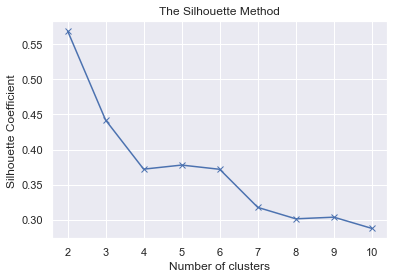
\includegraphics[width=10cm]{images_pfe/silhouette.png}
  \caption{Résultat de la méthode Silhouette.}
  \label{fig:silhouette-method}
\end{figure}
\FloatBarrier

La figure \ref{fig:silhouette-method} Lorem ipsum dolor sit amet, consectetur adipiscing elit. Proin posuere euismod neque, non semper nibh viverra sed. Praesent ut varius magna. Fusce ipsum ante, semper nec interdum at, semper et lacus. Nulla ultrices magna a fringilla finibus. Etiam sollicitudin blandit ante. Vivamus blandit rhoncus tincidunt. Morbi sit amet congue purus. Praesent interdum gravida congue. Donec fermentum dui fermentum maximus rutrum. $K = 2$ et ça rejoint le résultats de la méthode Elbow.

\medskip

Lorem ipsum dolor sit amet, consectetur adipiscing elit. Proin posuere euismod neque, non semper nibh viverra sed. Praesent ut varius magna.(Voir annexe \ref{app:pca}) Lorem ipsum dolor sit amet, consectetur adipiscing elit. Proin posuere euismod neque, non semper nibh viverra sed. Praesent ut varius magna.s (Voir annexe \ref{app:final-dataset}) . Lorem ipsum dolor sit amet, consectetur adipiscing elit. Proin posuere euismod neque, non semper nibh viverra sed. Praesent ut varius magna. (Voir figure \ref{fig:pca-method}). Les variables Lorem ipsum dolor sit amet, consectetur adipiscing elit. Nam massa magna, vulputate non sem eu, faucibus venenatis enim. Nullam sit amet pretium enim, sit amet condimentum magna. Mauris at pulvinar quam. Curabitur tincidunt tellus mi, auctor sodales nibh porttitor at. Aenean lobortis consequat aliquet. Suspendisse commodo euismod urna, eu finibus eros ultrices at. Donec ut dui nunc. Etiam ultrices ullamcorper ligula, ac tristique sapien scelerisque et. Donec sapien augue, vestibulum sit amet accumsan vel, varius eu odio.(Voir figure \ref{fig:correlation-circle}).


\begin{figure}[hbt!]
  \centering
  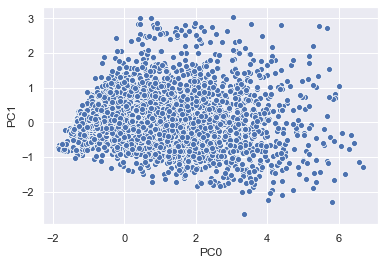
\includegraphics[width=10cm]{images_pfe/pca_results.png}
  \caption{Résultat de l'analyse en composantes principales.}
  \label{fig:pca-method}
\end{figure}
\FloatBarrier


Lorem ipsum dolor sit amet, consectetur adipiscing elit. Proin posuere euismod neque, non semper nibh viverra sed. Praesent ut varius magna. Fusce ipsum ante, semper nec interdum at, semper et lacus. Nulla ultrices magna a fringilla finibus. Etiam sollicitudin blandit ante. Vivamus blandit rhoncus tincidunt. Morbi sit amet congue purus. Praesent interdum gravida congue. Donec fermentum dui fermentum maximus rutrum. La figure \ref{fig:kmeans-pca}Lorem ipsum dolor sit amet, consectetur adipiscing elit. Proin posuere euismod neque, non semper nibh viverra sed. Praesent ut varius magna. Fusce ipsum ante, semper nec interdum at, semper et lacus. Nulla ultrices magna a fringilla finibus. Etiam sollicitudin blandit ante. Vivamus blandit rhoncus tincidunt. Morbi sit amet congue purus. Praesent interdum gravida congue. Donec fermentum dui fermentum maximus rutrum.

\begin{figure}[hbt!]
  \centering
  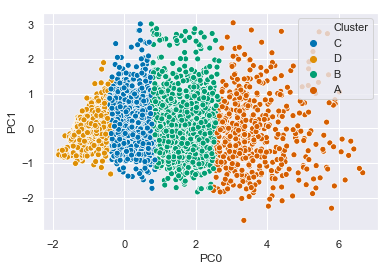
\includegraphics[width=10cm]{images_pfe/kmeans_clustering.png}
  \caption{Résultats de l'algorithme K-means en 2D (le cluster A en orange, B en vert, C en bleu et D en jaune).}
  \label{fig:kmeans-pca}
\end{figure}
\FloatBarrier

\subsection{Classification}
Lorem ipsum dolor sit amet, consectetur adipiscing elit. Proin posuere euismod neque, non semper nibh viverra sed. Praesent ut varius magna. Fusce ipsum ante, semper nec interdum at, semper et lacus. Nulla ultrices magna a fringilla finibus. Etiam sollicitudin blandit ante. Vivamus blandit rhoncus tincidunt. Morbi sit amet congue purus. Praesent interdum gravida congue. Donec fermentum dui fermentum maximus rutrum. (Voir les annexes \ref{app:random-forest}, \ref{app:svm}, \ref{app:naive-bays} et \ref{app:xgboost}). Pour évaluer ces différents algorithme nous avons utilisé le score $\text{F}_1$ moyen de toutes les classes (A, B, C et D). Le score $\text{F}_1$ est une mesure de la qualité de classification avec un score idéal égal à 1 . Le calcul du score $\text{F}_1$ d'une classe donnée se fait comme suit :
\begin{equation*}
    \text{F}_1 = 2 × \frac{\text{précision} ×  \text{rappel}}{\text{précision}+\text{rappel}}
\end{equation*}
avec :
\begin{equation*}
    \text{précision} = \frac{\text{Vrais positifs}}{\text{Vrais positifs}+\text{Faux positifs}}
\end{equation*}
et 
\begin{equation*}
    \text{rappel} = \frac{\text{Vrais positifs}}{\text{Vrais positifs}+\text{Faux négatifs}}
\end{equation*}

Un résultat est positif si sa classe prédite est la classe positive (ex: A), négatif sinon (ex: B, C ou D). Il est vrai si sa classe prédite correspond à sa classe réelle, faux sinon.


\begin{table}[h!]
    \centering
    \begin{tabular}{|c|c|c|}
        \hline
        Algorithme & score $\text{F}_1$ moyen  & score $\text{F}_1$ moyen avec validation croisée \\
        \hline
         Random Forest & 0.97 &  0.96 \\
        \hline
         SVM & 0.99 & 0.98 \\
        \hline
        Naive Bays & 0.94 &  0.94 \\
        \hline
        XGBoost & 0.98 &  0.97\\
        \hline
    \end{tabular}
    \caption{Évaluation des différents algorithmes de classification.}
    \label{tab:f1-scores}
\end{table}
\FloatBarrier


Le tableau \ref{tab:f1-scores} Lorem ipsum dolor sit amet, consectetur adipiscing elit. Proin posuere euismod neque, non semper nibh viverra sed. Praesent ut varius magna. Fusce ipsum ante, semper nec interdum at, semper et lacus. Nulla ultrices magna a fringilla finibus. Etiam sollicitudin blandit ante. Vivamus blandit rhoncus tincidunt. Morbi sit amet congue purus. Praesent interdum gravida congue. Donec fermentum dui fermentum maximus rutrum.

\subsection{Élaboration des plans de visite}
Lorem ipsum dolor sit amet, consectetur adipiscing elit. Proin posuere euismod neque, non semper nibh viverra sed. Praesent ut varius magna. Fusce ipsum ante, semper nec interdum at, semper et lacus. Nulla ultrices magna a fringilla finibus. Etiam sollicitudin blandit ante. Vivamus blandit rhoncus tincidunt. Morbi sit amet congue purus. Praesent interdum gravida congue. Donec fermentum dui fermentum maximus rutrum. (Voir \ref{tab:ptsp-results-comparison}). Le tableau ci-dessous illustre les différents résultats.


\begin{xltabular}{12cm}{|X|X|X|}
    \hline
    Instance & Notre algorithme     & MSC      \\\hline
    p01      &  440.94  & \textbf{432.10}   \\\hline
    p02      & 1118.70 & \textbf{1105.81}  \\\hline
    p03      & 494.45  & \textbf{466.71}   \\\hline
    p04      & 589.61  & \textbf{549.05}   \\\hline
    p05      & 1398.54 & \textbf{1382.33}  \\\hline
    p06      & 693.08  & \textbf{643.50}   \\\hline
    p07      & 670.34  & \textbf{643.80}   \\\hline
    p08      & 1645.90 & \textbf{1611.96}  \\\hline
    p09      & 838.06  & \textbf{720.72}   \\\hline
    p10      & 1310.29 & \textbf{1233.53}  \\\hline
    p11      & \textbf{490.95}& 490.97   \\\hline
    p12      & \textbf{664.07}  & 664.10   \\\hline
    p13      & 831.30  & \textbf{830.80}   \\\hline
    p14      & 996.86  & \textbf{994.60}   \\\hline
    p15      & 1159.94 & \textbf{1157.07}  \\\hline
    p16      & 664.21  & \textbf{649.96}   \\\hline
    p17      & 786.24  & \textbf{774.54}   \\\hline
    p18      & 886.94  & \textbf{873.73}   \\\hline
    p19      & 974.44  & \textbf{958.51}   \\\hline
    p20      & 1062.35 & \textbf{1033.58}  \\\hline
    p21      & \textbf{1374.88} & 1375.07 \\\hline
    p22      & 4321.96 & \textbf{4312.31}  \\\hline
    p23      & 8517.44 & \textbf{8308.48}  \\\hline
    pr01     & \textbf{2064.74} & 2064.84  \\\hline
    pr02     & 3220.29 & \textbf{3205.94}  \\\hline
    pr03     & 4065.70 & \textbf{4027.71}  \\\hline
    pr04     & 4609.59 & \textbf{4538.19}  \\\hline
    pr05     & 4706.05 & \textbf{4613.58}  \\\hline
    pr06     & 5633.53 & \textbf{5521.24}  \\\hline
    pr07     & 4472.17 & \textbf{4435.39}  \\\hline
    pr08     & 5457.90 & \textbf{5366.53}  \\\hline
    pr09     & 7352.93 & \textbf{7234.35}  \\\hline
    pr10     & 8360.00 & \textbf{8199.55}  \\\hline
    Diff \%  & 2.43    &    \\\hline 
    \caption{Comparaison entre les résultats de notre algorithme d'optimisation avec les meilleures solutions connues du PTSP}
    \label{tab:ptsp-final-results-comparison}
\end{xltabular}
\FloatBarrier

\medskip
Le tableau \ref{tab:ptsp-final-results-comparison} Lorem ipsum dolor sit amet, consectetur adipiscing elit. Proin posuere euismod neque, non semper nibh viverra sed. Praesent ut varius magna. Fusce ipsum ante, semper nec interdum at, semper et lacus. Nulla ultrices magna a fringilla finibus. Etiam sollicitudin blandit ante. Vivamus blandit rhoncus tincidunt. Morbi sit amet congue purus. Praesent interdum gravida congue. Donec fermentum dui fermentum maximus rutrum.

\medskip
Lorem ipsum dolor sit amet, consectetur adipiscing elit. Proin posuere euismod neque, non semper nibh viverra sed. Praesent ut varius magna. Fusce ipsum ante, semper nec interdum at, semper et lacus. Nulla ultrices magna a fringilla finibus. Etiam sollicitudin blandit ante. Vivamus blandit rhoncus tincidunt. Morbi sit amet congue purus. Praesent interdum gravida congue. Donec fermentum dui fermentum maximus rutrum. \parencite{noauthor_route_2020}. Lorem ipsum dolor sit amet, consectetur adipiscing elit. Proin posuere euismod neque, non semper nibh viverra sed. Praesent ut varius magna. Fusce ipsum ante, semper nec interdum at, semper et lacus. Nulla ultrices magna a fringilla finibus. Etiam sollicitudin blandit ante. Vivamus blandit rhoncus tincidunt. Morbi sit amet congue purus. Praesent interdum gravida congue. Donec fermentum dui fermentum maximus rutrum.




\subsection{Le dataflow Nifi}
Le but du dataflow Nifi est d'orchestrer et d'établir le lien entre les différentes parties du système. La figure \ref{fig:nifi-dataflow} Lorem ipsum dolor sit amet, consectetur adipiscing elit. Proin posuere euismod neque, non semper nibh viverra sed. Praesent ut varius magna. Fusce ipsum ante, semper nec interdum at, semper et lacus. Nulla ultrices magna a fringilla finibus. Etiam sollicitudin blandit ante. Vivamus blandit rhoncus tincidunt. Morbi sit amet congue purus. Praesent interdum gravida congue. Donec fermentum dui fermentum maximus rutrum.

\begin{figure}[hbt!]
  \centering
  \includegraphics[width=15cm]{images_pfe/NIFI_DATAFLOW.png}
  \caption{Dataflow Nifi.}
  \label{fig:nifi-dataflow}
\end{figure}
\FloatBarrier

\subsection{La plateforme de visualisation}
Lorem ipsum dolor sit amet, consectetur adipiscing elit. Proin posuere euismod neque, non semper nibh viverra sed. Praesent ut varius magna. Fusce ipsum ante, semper nec interdum at, semper et lacus. Nulla ultrices magna a fringilla finibus. Etiam sollicitudin blandit ante. Vivamus blandit rhoncus tincidunt. Morbi sit amet congue purus. Praesent interdum gravida congue. Donec fermentum dui fermentum maximus rutrum.

\medskip

Dans la page principale de la plateforme, nous retrouvons le tableau de bord (Voir figure \ref{fig:dashboard-page}). Lorem ipsum dolor sit amet, consectetur adipiscing elit. Proin posuere euismod neque, non semper nibh viverra sed. Praesent ut varius magna. Fusce ipsum ante, semper nec interdum at, semper et lacus. Nulla ultrices magna a fringilla finibus. Etiam sollicitudin blandit ante. Vivamus blandit rhoncus tincidunt. Morbi sit amet congue purus. Praesent interdum gravida congue. Donec fermentum dui fermentum maximus rutrum. \textit{POS} sous l'anglet \textit{Maps} (Voir figure \ref{fig:pos-page}). 

\medskip



\begin{figure}[hbt!]
  \centering
  \includegraphics[width=15cm]{images_pfe/dashboard.png}
  \caption{Tableau de bord de la plateforme.}
  \label{fig:dashboard-page}
\end{figure}
\FloatBarrier

\begin{figure}[hbt!]
  \centering
  \includegraphics[width=15cm]{images_pfe/pos_visualization.png}
  \caption{Visualisation des points de vente.}
  \label{fig:pos-page}
\end{figure}
\FloatBarrier

Lorem ipsum dolor sit amet, consectetur adipiscing elit. Proin posuere euismod neque, non semper nibh viverra sed. Praesent ut varius magna. Fusce ipsum ante, semper nec interdum at, semper et lacus. Nulla ultrices magna a fringilla finibus. Etiam sollicitudin blandit ante. Vivamus blandit rhoncus tincidunt. Morbi sit amet congue purus. Praesent interdum gravida congue. Donec fermentum dui fermentum maximus rutrum. \textit{Visits} sous l'anglet \textit{Maps} toujours (Voir figure \ref{fig:routes-settings-page}). Lorem ipsum dolor sit amet, consectetur adipiscing elit. Proin posuere euismod neque, non semper nibh viverra sed. Praesent ut varius magna. Fusce ipsum ante, semper nec interdum at, semper et lacus. Nulla ultrices magna a fringilla finibus. Etiam sollicitudin blandit ante. Vivamus blandit rhoncus tincidunt. Morbi sit amet congue purus. Praesent interdum gravida congue. Donec fermentum dui fermentum maximus rutrum. \textit{Routes} (Voir figure \ref{fig:routes-visualization-page}). Lorem ipsum dolor sit amet, consectetur adipiscing elit. Proin posuere euismod neque, non semper nibh viverra sed. Praesent ut varius magna. Fusce ipsum ante, semper nec interdum at, semper et lacus. Nulla ultrices magna a fringilla finibus. Etiam sollicitudin blandit ante. Vivamus blandit rhoncus tincidunt. Morbi sit amet congue purus. Praesent interdum gravida congue. Donec fermentum dui fermentum maximus rutrum.e \textit{Settings} (Voir figure \ref{fig:general-settings-page}). L'animateur de son coté, peut visualiser la route de chaque jour du plan et synchroniser les routes en temps réel (Voir figure \ref{fig:routes-visualization-page}).


\begin{figure}[hbt!]
  \centering
  \includegraphics[width=15cm]{images_pfe/visites_settings.png}
  \caption{Paramétrage des visites.}
  \label{fig:routes-settings-page}
\end{figure}
\FloatBarrier


\begin{figure}[hbt!]
  \centering
  \includegraphics[width=15cm]{images_pfe/route_visualization.png}
  \caption{Visualisation des itinéraires.}
  \label{fig:routes-visualization-page}
\end{figure}
\FloatBarrier

\begin{figure}[hbt!]
  \centering
  \includegraphics[width=15cm]{images_pfe/settings_page.png}
  \caption{Paramètres généraux.}
  \label{fig:general-settings-page}
\end{figure}
\FloatBarrier


\section{Conclusion}
Lorem ipsum dolor sit amet, consectetur adipiscing elit. Proin posuere euismod neque, non semper nibh viverra sed. Praesent ut varius magna. Fusce ipsum ante, semper nec interdum at, semper et lacus. Nulla ultrices magna a fringilla finibus. Etiam sollicitudin blandit ante. Vivamus blandit rhoncus tincidunt. Morbi sit amet congue purus. Praesent interdum gravida congue. Donec fermentum dui fermentum maximus rutrum.Lorem ipsum dolor sit amet, consectetur adipiscing elit. Proin posuere euismod neque, non semper nibh viverra sed. Praesent ut varius magna. Fusce ipsum ante, semper nec interdum at, semper et lacus. Nulla ultrices magna a fringilla finibus. Etiam sollicitudin blandit ante. Vivamus blandit rhoncus tincidunt. Morbi sit amet congue purus. Praesent interdum gravida congue. Donec fermentum dui fermentum maximus rutrum.





\chapter*{Conclusion and future outlook}

\label{sec:conclusion}

\clearpage

\section*{Conclusion}
In this thesis, we have developed and evaluated a robust end-to-end pipeline for automated skin lesion classification, based on a Mixture-of-Experts (MoE) architecture with Transformer-based feature extractors. Leveraging a balanced, augmented HAM10000 dataset and mixed-precision training on consumer-grade hardware, our model achieved 93\% overall accuracy and 84\% balanced accuracy on a held-out test set. Key innovations include dynamic expert routing, a load-balancing regularizer to ensure equitable expert utilization, and deployment-ready export to TorchScript/ONNX formats. These results demonstrate the viability of the MoE approach for dermatological image analysis, outperforming or matching state-of-the-art benchmarks while maintaining deployment flexibility.

\section*{Future outlook}
Building on these findings, future work will focus on transfer to clinical settings and advanced edge deployments. We plan to:
\begin{itemize}
  \item Integrate additional dermoscopic and non-dermoscopic datasets to improve generalization across imaging devices and populations.
  \item Incorporate patient metadata (age, lesion location, history) into the gating network to enhance diagnostic context.
  \item Evaluate post-training quantization and structured pruning on Coral Dev Boards with Edge TPUs for real-time, low-power inference.
  \item Explore semi-supervised and self-supervised techniques to leverage unlabeled clinical images and reduce annotation costs.
  \item Conduct prospective clinical validation studies to assess model impact on diagnostic workflow and patient outcomes.
\end{itemize}

%%% Local Variables: 
%%% mode: latex
%%% TeX-master: "isae-report-template"
%%% End:



%choix du style de la biblio

\printbibliography[nottype=misc,title={Bibliographie}]
 
\printbibliography[type=misc,title={Webographie}]





\appendix
\appendixpage




\clearpage
\thispagestyle{empty}




\end{document}
